% \documentclass[11pt, draft, twoside]{report}
\documentclass[12pt, twoside]{report}


\usepackage[utf8]{inputenc}                           % .tex Encoding spec
\usepackage[greek, francais]{babel}                   % language used
\usepackage{csquotes}                                 % Ensure correct quote text

% Text font pack
% \usepackage{charter}
% \usepackage{helvet}
\usepackage[scaled]{beramono}
% \usepackage[ttdefault=true]{AnonymousPro}              % only match source code
\usepackage[T1]{fontenc}                              % .pdf Encoding spec


% Template packages
\usepackage[top=2cm, bottom=2cm, left=2cm, right=2cm]{geometry}
\pagestyle{plain}                                     % Changing page style
\geometry{a4paper}                                    % Change page format

\usepackage{bookmark}                      % load hyperref internaly
\hypersetup{
    pdfkeywords={Passive,
                 Optimisation,
                 Solaire,
                 Système combiné},         % list of keywords
    unicode=true,                          % non-Latin characters in Acrobat’s bookmarks
    pdftoolbar=true,                       % show Acrobat’s toolbar?
    pdfmenubar=true,                       % show Acrobat’s menu?
    pdffitwindow=false,                    % window fit to page when opened
    pdfstartview={FitH},                   % fits the width of the page to the window
    pdftitle={Outil d’aide à la décision
              pour la construction de
              maison passives
              100\% solaires},             % title
    pdfauthor={Jérémy Bois},               % author
    pdfsubject={Optimisation,
                Maison passive},           % subject of the document
    pdfcreator={Jérémy Bois},              % creator of the document
    pdfproducer={Jérémy Bois},             % producer of the document
    pdfnewwindow=true,                     % links in new PDF window
    colorlinks=true,                       % false: boxed links; true: colored links
    linkcolor=orange,                      % color of internal links (change box color with linkbordercolor)
    citecolor=magenta,                     % color of links to bibliography
    filecolor=magenta,                     % color of file links
    urlcolor=cyan                          % color of external links
}

% Pretty printer packages
\usepackage{listings}                                 % Intern or extern sources

% Appendix package to add sub-annex and annex to main table
\usepackage{appendix}

% Color packages
\usepackage[dvipsnames, svgnames]{xcolor}
\newcommand{\NOTE}[1]{\relax\let\next\allowbreak\colorbox{blue!30}{#1}}        % Add a background to notes

% Add support for image and defines image folder
\usepackage{./Template/ImagesFolder}

% Easy pro tables
\usepackage{booktabs}

% Allow to create tab on multiple pages
\usepackage{longtable}

% Set new longer caption size
\setlength{\LTcapwidth}{8in}

% Centering multirows
\newcommand{\minitab}[2][c]{\begin{tabular}{#1}#2\end{tabular}}

% Best tab formatter
\usepackage{tabulary}

% Multiple row
% \usepackage{multirow}

% Unit package
\usepackage{siunitx}

% Allow adding complex equations
% (\times, \div) compute multi and div (Used if encoding in utf8)
\usepackage{amsmath}

% Turn off french bulleted lists (-) ---> Private format : \item[\textbf{--}]
\frenchbsetup{StandardLists=true}

% Add bibliography and reference in the citation order
\usepackage[style=authoryear,sorting=none, backend=biber]{biblatex}
\addbibresource{Bibliographie/references.bib}

% Title page
\title{
    {Outil d’aide à la décision pour la construction de maisons passives 100\% solaires}\\
    {\large Université de Bordeaux}\\
    {\includegraphics{Logos/aquitaine_logo.png}}
}
\author{Jérémy Bois}
\date{}

% Limit included files
\includeonly{Chapitres/Chap2-Modelisation, Chapitres/Chap3-UnOutilAideDecision,
             Chapitres/Chap4-OptimisationSystemeSolaire}

% ------------------------------------------------------------------------------
% Document start here
% ------------------------------------------------------------------------------
\begin{document}

% First page
\pagenumbering{Alph}
\begin{titlepage}
    \maketitle
    \thispagestyle{empty}
\end{titlepage}
\pagenumbering{arabic}


% % Other stuff
% \chapter*{Résumé}
% Résumé ici

% \chapter*{Remerciements}
% Merci merci ...


\tableofcontents
\listoffigures
\listoftables
\thispagestyle{empty}
\newpage


% Start importing chapters
\chapter*{Introduction}
%!TEX root = ../main.tex

Oui c’est ça c’est l’introduction ...


\chapter{Contexte des travaux}
%!TEX root = ../main.tex
% Chapitres\Chap1-ContexteTravaux.tex


% % ...........................................................................
% % ...........................................................................
% \section{Objectifs de ces travaux} % (fold)
% \label{sec:objectifs_de_ces_travaux}
% \itodo{Ajouter section objectifs}

% \itodo{Voir Hugo Stéphanie et thomas}

% \iunsure{Utile de le mettre ici seulement à la fin}
% % section objectifs_de_ces_travaux (end)


\itodo{Vérifier accords avec auteurs}



% ...........................................................................
% ...........................................................................
\section{L’Homme au centre d’un trouble climatologique} % (fold)
\label{sec:l_homme_au_centre_d_un_trouble_climatologique}
% ------------------------------------------------------------------------------
\subsection{Le réchauffement climatique~: origines et conséquences} % (fold)
\label{sub:le_rechauffement_climatique_origines_et_consequences}
Auparavant les différentes tâches étaient principalement réalisées soit en utilisant les
éléments (vent, eau, feu) soit en utilisant la force animale (bœufs, chevaux\dots). Les
révolutions industrielles marquent l’émergence des machines, la société passe alors d’une
dominante artisanale et agraire à une société commerciale et industrielle affectant aussi
bien l’agriculture que la politique ou l’économie. Dès le début des années $1990$ le
pétrole devient une source énergétique (\defref{def:energie}) stratégique et est
activement utilisé dans l’industrie. La tendance s’accélère après la seconde guerre
mondiale, durant la période des $30$ glorieuses, où la France et d’autres pays développés
profitent d’une croissance forte tant au niveau économique, que démographique (baby-boom).
Cette expansion est portée par un accès aisé aux énergies et particulièrement aux énergies
fossiles principaux vecteur de développement de nos civilisations occidentales. Durant
cette période marquée par le développement du capitalisme, une énergie bon marché
considérée comme inépuisable, et un accroissement important de la population, la demande
énergétique explose. Afin de pouvoir comparer les différentes énergies entre elles, une
unité commune est retenue~: le tonne équivalent pétrole (\abr{tep}) ou tonnes of oil
equivalent (\abr{toe}) dans sa version anglophone qui équivaut au pouvoir calorifique
d’une tonne de pétrole, soit \SI{41.868}{\giga\joule}.
À titre de comparaison, l’énergie primaire consommée en $1973$ était de
\SI{6101}{\mega tep} dont \SI{87}{\percent} en énergie fossile alors qu’elle est en $2014$
à \SI{13699}{\mega tep} pour une part de près de \SI{81}{\percent} en énergie fossile
(\figref{fig:energy_fraction}). Il peut ainsi être noté que cette énergie
reste aujourd’hui encore fortement majoritaire même si la consommation du pétrole diminue.

\begin{figure}
    \centering
    \includegraphics{Ressources/Images/Environnement/repartition_energy.png}
    \caption{Répartition des sources de production en énergie primaire pour
             $1973$ et $2014$ d’après \textcite{IEA2016} (\enquote{other} comprend
             la géothermie, le solaire, et l’éolien).}
    \label{fig:energy_fraction}
\end{figure}


Une fraction de cette énergie est utilisée pour le chauffage, la voiture, ou encore pour
nos équipements électriques de plus en plus nombreux~: \SI{+41}{\percent}
entre $2010$ et $2013$ pour la France \textcite{ADEME2015}. L’autre fraction moins visible est
pourtant majoritaire, c’est l’énergie utilisée pour la production, le transport ou le
stockage des biens de consommation de la vie courante.
La sur exploitation de ces énergies montre cependant des limites et impacte de manière
importante l’environnement.

\begin{Def}[Énergie]\label{def:energie}
Dans l’ensemble de ce document, le terme énergie réfère non à son sens moral mais à son
sens physique. L’énergie en physique est la mesure de la capacité d’un système à produire
de la chaleur, modifier un état, ou encore entraîner un mouvement. Dans notre
problématique une distinction est nécessaire entre l’énergie dite \textbf{primaire} et
l’énergie dite \textbf{finale}. L’énergie primaire correspond à l’énergie prélevée à
l’environnement alors que l’énergie finale est l’énergie primaire après soustraction des
pertes de stockage, de transport, et de transformation. L’énergie finale correspond ainsi
à l’énergie consommée par l’utilisateur sans tenir compte des consommations engendrées pour sa
production à l’opposée de l’énergie primaire. Le bouquet énergétique étant propre à chaque
pays, les facteurs de conversion le sont eux aussi. Pour la France,
les coefficients souvent admis sont définis en annexe (\tabref{tab:coef_finale_primaire}).
\end{Def}

Les effets du réchauffement climatiques sont aujourd’hui facilement observables et sont
tels qu’ils bouleversent le fonctionnement de la planète. Bien que nous soyons en période
de réchauffement (causes externes astronomiques) l’impact de l’être humain est aujourd’hui
reconnu. La sur-utilisation des énergies fossiles couplée à une forte évolution
démographique se traduit par de trop fortes émissions en Gaz dits \enquote{à Effet de
Serre (\defref{def:effet_serre})} (\abr{GES}). Actuellement les mesures montre un forçage
radiatif excédentaire entraînant une lente augmentation de la température du sol
terrestre. Entre $1750$ et $2005$, ce forçage est estimé à
\SI{2.63}{\watt\per\metre\squared} dont \SI{1.6}{\watt\per\metre\squared} imputable aux
émissions anthropiques (\cite{Myhre2013}, tableau 8.6). La température moyenne sur
l’ensemble de la surface du globe étant le résultat du bilan radiatif entre le rayonnement
solaire incident et le rayonnement infrarouge terrestre émis, elle augmente lorsque la
part du rayonnement terrestre émis puis absorbé par l’atmosphère augmente. La vapeur
d’eau contribue à \SI{55}{\percent} à l’effet de serre et apparaît ainsi comme le
principal responsable. Cependant, il n’est donc pas considéré lors de
l’étude des émissions de
\abr{GES} anthropiques car l’Homme n’a pas un impact direct sur sa concentration dans l’atmosphère.
L’étude des émissions anthropiques peut donc être assimilée à l’étude des émissions
néfastes additionnelles aux émissions naturelles. Dans des conditions normales l’effet de
serre est en effet positif et permet de maintenir une température correcte pour le
développement de la biodiversité~: en son absence la température moyenne de la terre
serait de \SI{-18}{\celsius}. En conséquence, l’effet de serre additionnel est en majorité
due à la concentration de $CO_{2}$ avec \SI{56.6}{\percent}, mais aussi au méthane
($CH_{4}$), au protoxyde d’azote ($N_{2}O$) et à l’ozone (O3).
\figref{fig:evolution_effet_serre} met en évidence l’accélération
des consommations à partir de $1950$ qui se traduit par une forte
augmentation de la concentration de $CO_{2}$ dans l’atmosphère.

\begin{Def}[Effet de serre]\label{def:effet_serre}
C’est un phénomène naturel engendré par la présence de divers composés
gazeux dans l’atmosphère. L’atmosphère ayant un faible indice de réflexion et d’absorption
pour le rayonnement solaire (visible, proche \abr{UV} et proche \abr{IR}), une grande
partie du rayonnement est transmise à la surface de la terre. Une fraction est alors
absorbée alors qu’une autre est réfléchie et repart dans l’espace. La part absorbée
engendre un échauffement, le sol émet alors un rayonnement dans le domaine de l’\abr{IR}
lointain. Certains composants gazeux de l’atmosphère étant faiblement transparents pour ce
domaine d’émission, une partie de l’énergie est absorbée au lieu d’être rejetée dans
l’espace~: c’est le mécanisme d’effet de serre.
\end{Def}

\begin{figure}
    \centering
    \includegraphics{Ressources/Images/Environnement/evolution_effet_serre.png}
    \caption{Évolution de la concentration des principaux \abr{GES} au cours des
             derniers siècles \parencite{IPCC2014}.}
    \label{fig:evolution_effet_serre}
\end{figure}

L’activité humaine depuis la révolution industrielle amène aujourd’hui à un taux de
concentration en \abr{GES} jamais atteint depuis près de \SI{800000}{ans}
\parencite{IPCC2014}.
Bien que non imputables en totalité au réchauffement climatique, les événements extrêmes
attribués au changement climatique sont de plus en plus nombreux et touchent l’ensemble
des écosystèmes, faune comme flore (\cite{IPCC2014}, Figure SPM.4).
L’augmentation des occurrences de canicules, des fortes précipitations, ou
l’élévation du niveau de la mer font notamment partie des conséquences
directes. Cependant, le mode de développement actuel de l’être humain (transport, bâtiment, population, robotisation\dots)
est aussi responsable de nombreux autres facteurs environnementaux aggravants, comme l’acidification des sols,
la pollution de l’air, la réduction de la biodiversité\dots \parencite{Biermann2016341}.
Il a ainsi mis en évidence d’une part l’effet néfaste du réchauffement climatique
et d’autre part la forte influence humaine au cours de la dernière décennie (\figref{fig:evolution_climat}).
Lorsque seul les émissions naturelles sont considérées, les résultats de simulations
mettent en effet clairement en évidence une stagnation de la température moyenne. À
l’inverse les observations et simulations qui tiennent compte de la part anthropique
montrent que l’énergie stockée dans les océans (\abr{OHC}, Ocean Heat Content), la température des océans comme de la
terre, ou encore la fonte des glaces en Arctique sont imputables à l’être humain.
Des mesures doivent ainsi être prises afin de limiter la consommation en énergie primaire
et les émissions en \abr{GES}. L’énergie étant cependant indispensable pour notre mode de
vie actuelle, une alternative respectueuse de l’environnement, les énergies renouvelables, réduisant les émissions de
\abr{GES} est indispensable pour permettre d’inverser la tendance.

\begin{figure}
    \centering
    \includegraphics{Ressources/Images/Environnement/elevation_temperature.jpg}
    \caption{Mise en évidence des effets anthropiques globaux et à l’échelle de la région
              à travers l’évolution des température des océans et des terres, des précipitations,
              de l’énergie stockée dans les océans (\abr{OHC}, Ocean Heat Content), et
              de la surface de mer gelée. Les lignes rouges et bleues foncées représentent l’évolution moyenne
              des différentes simulations respectivement avec et sans influence humaine. Les zones
              ombrée en bleu et rose représentent les intervalles de confiance pour les différentes
              simulations. Finalement les lignes de teintes grises décrivent les observations
              de différents travaux \parencite{AchutaRao2013}.
             }
    \label{fig:evolution_climat}
\end{figure}
% subsection le_rechauffement_climatique_origines_et_consequences (end)

% ------------------------------------------------------------------------------
\subsection{Vers une prise de conscience collective} % (fold)
\label{sub:vers_une_prise_de_conscience_collective}
Aujourd’hui visible, les effets majeurs du dérèglement climatique trouvent leur origine au
$20ème$ siècle durant la révolution industrielle. En $1970$, le club de Rome commandite le
rapport Meadows \enquote{Halte à la croissance ?}, publié en $1972$
\parencite{Meadows1972}. Pour la première fois, la possibilité d’une pénurie des
ressources énergétiques est envisagée par des chercheurs du \abr{MIT} à travers plusieurs
scénarios plus ou moins catastrophiques. Ce rapport fut la première pierre nécessaire à la
construction d’une prise de conscience commune et sera ensuite mis à jour à plusieurs
reprises. L’être humain commence alors à prendre conscience de son impact sur
l’environnement et des problèmes qu’il engendre~: destruction de la couche d’ozone,
gestion des déchets, bouleversement climatiques, pollution de l’eau, atteintes à la bio-
diversité\dots En $1987$ un nouveau rapport cette fois commandité par les Nations Unies,
\enquote{Notre avenir à tous}, plus connu sous le nom de rapport \textit{Bruntland} \parencite{Brundtland1987}.
Contrairement au rapport \textit{Meadows} qui présente des scénarios de ce qui pourrait
arriver si rien ne change, ce document pose les bases pour un développement équitable
mettant en avant la protection des ressources naturelles mais aussi de l’équité des
individus face aux ressources. Le terme \enquote{Développement durable} (\figref{fig:developpement_durable},
aujourd’hui largement repris, est introduit~:

\blockquote{
    Un développement qui répond aux besoins du présent sans
    compromettre la capacité des générations futures à répondre aux leurs.
}

\begin{figure}
    \centering
    \begin{subfigure}[b]{0.55\textwidth}
        \centering
        \includegraphics{Ressources/Images/Environnement/developpement_durable.png}
        \caption{}
        \label{fig:developpement_durable}
    \end{subfigure}
    \quad
    \begin{subfigure}[b]{0.4\textwidth}
        \centering
        \includegraphics{Ressources/Images/Environnement/triptyque_negaWatt.png}
        \caption{}
        \label{fig:negawatt_axes}
    \end{subfigure}
    \caption[Principe du développement durable et du scénario négaWatt]
             {Principe du développement durable \protect\footnotemark (a). Principe du
              scénario \textit{négaWatt} (b) \parencite{Salomon2012}.}
    \label{fig:developpement_durable_negawatt}
\end{figure}
\footnotetext{\url{http://www.cdcmortainais.fr}}

% \begin{figure}
%     \centering
%     \includegraphics{Ressources/Images/Environnement/developpement_durable.png}
%     \caption[Principe du développement durable]
%             {Principe du développement durable \protect\footnotemark}
%     \label{fig:developpement_durable}
% \end{figure}

Au début portée par des militants, la conscience collective amène à la prise en compte de
l’environnement dans les textes réglementaires avec notamment le \textit{protocole de
Montreal} ($1987$) mettant en place des restrictions afin de protéger la couche d’ozone.

Les décisions politiques étant étroitement liées aux résultats scientifiques,
une organisation indépendante a été créé en $1988$ par l’Organisme des Nations
Unies (\abr{ONU}) afin de fournir une base scientifique solide. Cette organisation connue sous le nom de
Groupe d'experts Intergouvernemental sur l'Évolution du Climat (\abr{GIEC}), regroupe
des experts en climatologie dont le but est d’apporter un regard critique sur
les travaux provenant de différents groupes de recherche scientifiques, techniques,
et socio-économiques. Il a pour but la réalisation sans parti-pris de l’expertise
des risques liés au réchauffement climatique et de faire re-sortir les informations
et découvertes faisant consensus dans la communauté scientifique. Finalement, grâce à ces
publications périodiques, les connaissances accumulées sur le sujet permettent de
sensibiliser le public non expert, élément indispensable pour que des engagements
politiques soit pris.

Peu de temps après, au $3ème$ \textit{Sommet de la Terre} se tenant à Rio en $1992$, la
Convention-Cadre des Nations Unies sur les Changements Climatiques
(\fnref{http://unfccc.int/essential_background/convention/status_of_ratification/items/2631.php}{\abr{CCNUCC}})
est adoptée. Cette convention développe un plan d’action pour le $21ème$ siècle,
l’\textit{Agenda $21$} mais aussi $27$ principes pour sa mise en œuvre. Les domaines
traités sont très variés et couvrent par exemple la pauvreté, la gestion des ressources
notamment en eau, des déchets, mais aussi la pollution ou l’agriculture\dots Elle est
ensuite complétée par un accord visant à réduire les émissions de gaz à effet de serre
(\abr{GES}) lors de la $3ème$ Conférence des Parties (\abr{COP}, Conference Of Parties) à
Kyoto ($1997$) avec une entrée en vigueur début $2005$. La \abr{CCNUCC} est aujourd’hui
ratifiée par $197$ pays montrant l’intérêt des questions du développement durable sur le
plan international. Pour la première fois, en $2006$, le \textit{rapport Stern}
\parencite{Stern2006} commandé par le gouvernement britannique décrit sur le plan
économique l’impact d’une inaction face aux problèmes du réchauffement climatique.
Précédemment mis en avant par des scientifiques, la sonnette d’alarme est ici tirée par un
économiste mettant en avant les risques tant sur le plan humain que économique. Le
réchauffement impacte en effet directement les composantes essentielles de notre mode de
vie~: l’accès à la santé, à la nourriture ou encore à l’eau. Il est alors suggéré un effort
de recherche et une coopération technique au niveau international afin de répondre à la
problématique de manière efficace. Il est aussi mis en avant la nécessité pour les pays
riches, principaux responsables du réchauffement climatique, d’aider au développement des
pays plus pauvres dans des conditions respectueuses de l’environnement.

Dès $2007$, la réunion entre gouvernements et chefs d’états de l’Union Européenne
(\abr{EU}) définissent des objectifs globaux pour $2020$. Ces objectifs sont au cœur du
\fnref{http://www.assemblee-nationale.fr/13/europe/rap- info/i1260.asp}{paquet climat-
énergie} et engage l’Europe à réduire de \SI{20}{\percent} (par rapport à $1990$) ces
émissions de \abr{GES}, à améliorer de \SI{20}{\percent} l’efficacité énergétique, et à
couvrir \SI{20}{\percent} de la consommation finale par des énergies renouvelables
(\abr{EnR}). Au niveau international, la $21ème$ \abr{COP} ($2016$) a permis d’aller
encore plus loin avec l’acception de la mise en place de mesures pour la réduction des
émissions de \abr{GES} avec notamment l’objectif de contenir le réchauffement climatique
en dessous des \SI{2}{\degree} (réalisation du plan facteur $4$) À terme, le respect de la trajectoire
permettra d’atteindre la \enquote{neutralité carbone} en compensant les émissions de
\abr{GES} dans la seconde moitié du siècle. Contrairement au précédent accord
(\textit{Accords de Kyoto}), le parti-pris est ici d’imposer une transparence entre les
différents signataires. Chaque signataire doit ainsi rendre compte régulièrement des
objectifs et évolutions réalisées, informations qui seront disponibles publiquement afin
d’inciter à l’exemplarité. Ancrées d’une forte symbolique et marquant un pas important vers
un développement plus durable, aucunes prises de mesures ne sont cependant obligatoires et
la sobriété énergétique n’est pas mentionnée.


\subsubsection{Le cas français} % (fold)
\label{ssub:le_cas_francais}
En France, l’engagement \enquote{facteur 4} ($2003$) et le paquet climat-énergie défini
au niveau européen sont repris dans les objectifs des lois \textit{Grenelle I et II}
\parencite{Grenelle2010}. Ce texte traduit pour la France une volonté de décisions sur le
long terme à la fois sur le plan sociétal, politique, et économique, même si la question
du nucléaire n’est pas encore à l’ordre du jour. Ces lois marquent le premier pas vers une
démarche responsable sur les transports, la santé, l’énergie ou encore la préservation de
la bio-diversité comme notamment avec la labellisation de l’agriculture BIO ou la
réduction de la précarité énergétique des foyers. Ces mesures s’appuient notamment sur le
plan de transition énergétique proposé par l’association \textit{négaWatt}
\parencite{Salomon2012}.

\textit{NégaWatt} est une association française qui développe depuis $2003$ un scénario de
transition énergétique permettant à l’horizon $2050$ de couvrir les besoins énergétiques à
\SI{100}{\percent} grâce aux énergies renouvelables~: biomasse, éolien, solaire \parencite{negaWatt2017}. La
trajectoire proposée suit trois axes principaux (\figref{fig:negawatt_axes})~: plus de
sobriété, améliorer l’efficacité énergétique, promouvoir les énergies renouvelables.
L’association regroupe dans cet objectif, des experts du domaine de l’énergie, des
économistes, des sociologues\dots, et tient compte des données statistiques sur des
domaines multiples comme l’évolution démographique, la consommation des foyers, le coût
des énergies\dots La sobriété élément clé du scénario invite à repenser son mode de vie et
propose ainsi à la fois une transition énergétique mais aussi comportemental basé sur un
principe simple à l’origine du mot \textit{négawatt}~:
\blockquote{L’énergie qui pollue le moins est celle que l’on ne consomme pas.}
Parmi les nombreuses mesures concrètes proposées, il peut être cité, l’amélioration des transports en
commun, la réduction des dépenses électriques inutiles, l’isolation du bâti existant,
l’économie circulaire, ou encore un programme de sortie progressive du nucléaire pour
$2035$.

% \begin{figure}
%     \centering
%     \includegraphics{Ressources/Images/Environnement/triptyque_negaWatt.png}
%     \caption{Principe du scénario \textit{négaWatt} d’après \textcite{Salomon2012}.}
%     \label{fig:negawatt_axes}
% \end{figure}

Depuis $2012$, au niveau de l’agriculture et donc de l’accès à la nourriture, le scénario \textit{négaWatt}
est complété par le scénario \textit{Afterres2050} développé par l’\abr{ONG} \textit{Solagro}. Ce
scénario s’intéresse principalement à la gestion des forêts, la biodiversité, ou encore
les terres agricoles afin de nourrir de manière durable la population française.
Le scénario met notamment en avant que le respect du facteur $4$ couplé à une alimentation
et une agriculture plus raisonnées permettrait de couvrir les besoins alimentaires
de l’ensemble des français. S’appuyant aussi sur le principe de sobriété, le scénario
indique aussi que une réduction par deux de la consommation de viande est
nécessaire afin d’une part de réduire les émissions de gaz à effet de serre mais
aussi afin de libérer des terres pour la production de biomasse.
Le travail de ces associations est rapidement reconnu et s’inscrit en $2015$ dans le cadre de
de la Loi pour la Transition Énergétique et la Croissance Verte
(\fnref{https://www.legifrance.gouv.fr/affichTexte.do?cidTexte=JORFTEXT000031044385}{\abr{LTECV}})
comme un des scénarios de maîtrise de l’énergie au coté du scénario de l’\textit{ADEME}
basée sur l’efficacité, du scénario \textit{ANCRE} basé sur la diversité des énergies, et du scénario \textit{Négatep}
basé sur la dé-carbonisation.
La loi décrit ainsi de nombreux engagements visant à réduire l’impact de l’homme sur le
climat, créer de l’emploi pour une population grandissante, mais aussi réduire la précarité
avec un plan de rénovation du patrimoine bâti. Des engagement forts sont ainsi pris au
niveau énergétique et environnemental pour $2030$~:
\begin{itemize}
    \item réduire de \SI{40}{\percent} (par rapport à $1990$) les émissions des gaz a
          effet de serre et par quatre à l’horizon $2050$.
    \item réduire de \SI{20}{\percent} (par rapport à $2012$) la consommation en énergie
          finale et de \SI{-50}{\percent} pour $2050$.
    \item réduire de \SI{30}{\percent} la consommation en énergie primaire.
    \item porter à \SI{32}{\percent} la part des \abr{EnR} sur la consommation finale brute.
    \item réduire la dépendance à l’énergie nucléaire pour la production d’électricité à
          \SI{50}{\percent} évaluée à \fnref{http://tinyurl.com/y7ujs7dn}{\SI{77}{\percent}} en $2014$
\end{itemize}
% subsubsection le_cas_francais (end)
% subsection vers_une_prise_de_conscience_collective (end)
% section l_homme_au_centre_d_un_trouble_climatologique (end)





% ..............................................................................
% ..............................................................................
\section{Vers le bâtiment à énergie positive} % (fold)
\label{sec:vers_le_batiment_a_energie_positive}
% ------------------------------------------------------------------------------
\subsection{Un long chemin déjà parcouru} % (fold)
\label{sub:un_long_chemin_deja_parcouru}
Représentant la majeure partie des consommations en énergie dans le monde, le secteur du
bâtiment a un rôle déterminant à jouer dans le respect des engagements politiques. En
France selon \textcite{ADEME2015}, le secteur du bâtiment est responsable à
\SI{45}{\percent} des consommations en énergie finale devant les transport
(\SI{33}{\percent}) et l’industrie (\SI{19}{\percent})
(\figref{fig:evolution_energy_finale}). C’est de plus le troisième secteur le plus
polluant avec \SI{20}{\percent} des émissions en $CO_{2}$(eq) derrière
l’industrie (\SI{30}{\percent}) et les transports (\SI{28}{\percent}).


\begin{figure}
    \centering
    \begin{subfigure}[b]{0.45\textwidth}
        \includegraphics{Ressources/Images/Environnement/evolution_energie_finale.png}
        \caption{}
        \label{fig:evolution_energy_finale}
    \end{subfigure}
    \quad
    \begin{subfigure}[b]{0.45\textwidth}
        \includegraphics{Ressources/Images/Environnement/repartition_energy_primaire.png}
        \caption{}
        \label{fig:repartition_conso_primaire}
    \end{subfigure}
    \caption[Description du secteur énergétique français]
             {Évolution de la consommation française en énergie finale (a) et
              répartition de la consommation française en énergie primaire en $2012$ (b)
              d’après \textcite{ADEME2015}}
    \label{fig:energy_france}
\end{figure}

C’est suite au premier choc pétrolier de $1973$ que la France met en place en $1974$ la première
Réglementation Thermique (\abr{RT}) afin de faire face aux dépenses énergétiques importantes
dans le secteur du bâtiment. L’énergie qui hier semblait inépuisable apparaît
alors comme une ressource limitée et la sécurité de l’approvisionnement devient une
préoccupation nationale. D’après l’\abr{ADEME}, la consommation annuelle en énergie finale est
alors de l’ordre de \SI{370}{kWh\per\metre\squared} dans le secteur du résidentiel et la
réglementation fixe un objectif de réduction de la consommation de
\SI{25}{\percent}. Une méthodologie de calcul commune est aussi mise en place et
un contrôle régulier des systèmes de chauffage comme de climatisation imposée.
Cette réglementation évolue ensuite en $1982$, $1989$, puis $2000$ portée par
les différents acteurs du secteur du bâtiment.

Dans une approche volontariste, les états européens adoptent en $2002$, la directive sur la
performance énergétique des bâtiments (\abr{2002/91/EC}, \cite{EPBD2002}) qui fut à
l’origine d’avancées significatives pour tous les états membres avec notamment la mise en
place des diagnostics de performance énergétique (\abr{DPE}), des valeurs seuils et une
méthodologie commune pour évaluer la performance énergétique des bâtiments, le contrôle
régulier des chaudières (\SI{+10}{kW}) et un effort de normalisation commune par le Comité
Européen de Normalisation (\abr{CEN}).
Ces engagements ont été traduit par la plupart des pays membres dans leur \abr{RT}
propre comme la France à travers les
disposition des lois Grenelle et les \abr{RT}\,$2005$.
Mise en application en $2006$, elle marque de nombreuses avancées
réglementaires notamment avec l’introduction du concept de bâtiment de référence. Chaque
bâtiment est ainsi évalué par rapport à la référence et des gardes-fous sont mis en place
afin d’éviter les incohérences énergétiques. De plus la construction bioclimatique avec
l’intégration des énergies renouvelables dans la méthode de calcul ou encore l’évaluation
du confort d’été sont maintenant pris en compte.
Ces mesures incitatrices sont aussi à l’origine de la publication dans le journal officiel
en mai $2007$ de l’arrêté encadrant l’obtention d’un label \abr{HPE} qui permet de valoriser
un bâtiment obtenant un niveau de performance globale supérieur à la \abr{RT}.
Le label comporte cinq niveaux dont le plus performant, le label Bâtiment à
Basse Consommation (\fnref{https://www.effinergie.org/web/index.php/les-labels-effinergie/bbc-effinergie}{\abr{BBC}-$2005$})
est inspiré du label Suisse \textit{Minergie}. Pour la première fois en France, un
label d’excellence énergétique est proposé et impose une consommation en énergie primaire
sur le chauffage, la production d’\abr{ECS}, le refroidissement, et l’éclairage à
\SI{50}{kWh\per\metre\squared} (modulé en fonction des conditions géographiques).
La mise en place de ce label a permis aux professionnels de s’adapter aux contraintes
énergétiques fortes qui seront repris dans la réglementation actuellement en vigueur, la
\abr{RT}\,$2012$.
En effet le passage à la \abr{RT\,$2012$} impose aux bâtiments une consommation maximale (\abr{$C_{ep}$\,max})
réduite de moitié. De plus le nouveau seuil tient aussi compte de l’éclairage et des auxiliaires alors
que dans la \abr{RT\,$2005$}, le \abr{$C_{ep}$\,max} est définie uniquement pour le
chauffage, la production d’\abr{ECS}, et le refroidissement. Les travaux se concentre
aujourd’hui sur la préparation de la \abr{RT\,2020}, qui devra permettre d’honorer les
engagements européens et se rapprocher des objectifs internationaux pour $2030$ et $2050$.

\subsubsection{La place de la maison individuelle} % (fold)
\label{ssub:la_place_de_la_maison_individuelle}
Si on considère uniquement le parc résidentiel, la consommation moyenne
est de \SI{186}{\kWh_{ep}\per\metre\squared} en $2012$ dont \SI{67}{\percent} dû
au chauffage. Les ménages représentent ainsi \SI{25}{\percent} des consommations
en énergie primaire (\figref{fig:repartition_conso_primaire}). Finalement malgré
une réduction de la consommation moyenne des logements jusqu’en $2006$, la
consommation augmente entre $2002$ et $2012$. Il est donc important
de faire des économies d’énergie dans le bâtiment et en particulier dans le résidentiel
afin d’une part de respecter les engagements mais aussi réduire la facture énergétique.
D’après l’Institut National de la Statistique et des Études Économiques (\abr{INSEE})
la maison individuelle représente en $2016$ \SI{56}{\percent} des \SI{35}{milliers}
logements en France.
Rénover le patrimoine existant est la mesure la plus importante afin de réduire
les consommations en énergie fossile, réduire notre dépendance à l’énergie nucléaire,
et limiter les émissions de \abr{GES}. Il est cependant important de continuer à
innover dans le neuf et par extension dans la maison individuelle.
Malgré une diminution en faveur des habitats collectifs depuis $2008$, la maison individuelle
représente en effet près de \num{200000} nouveaux chantiers terminés par an dont $\nicefrac{3}{4}$
de maisons individuelles pures \parencite{Caicedo2015}.
Ainsi les nouvelles constructions de maisons individuelles se doivent d’êtres innovantes
énergétiquement afin de proposer des solutions économiquement viables et performantes
pour la rénovation.
% subsubsection la_place_de_la_maison_individuelle (end)
% subsection un_long_chemin_deja_parcouru (end)



% ------------------------------------------------------------------------------
\subsection{Description générale du concept} % (fold)
\label{sub:description_generale_du_concept}
% \href{Further development of EU energy efficiency policies}{http://tinyurl.com/yafjydu7}

Bien qu’il n’existe pas encore de cadre réglementaire en France,
la directive européenne \abr{2010/31/EU} \parencite{EPBD2010} (mise à jour de \textcite{EPBD2002})
décrit un programme commun pour les pays de l’\abr{EU}.
Elle introduit le concept \enquote{nearly Zero Energy Buildings}
(\textit{nearly}\,\abr{ZEB}) incitant chaque état membre à mettre en
œuvre une politique permettant d’atteindre pour tous les bâtiments neufs une consommation
énergétique en énergie primaire \enquote{quasi nulle} en $2018$ pour les bâtiments publics
et en $2020$ pour le privé (article $2$ et $9$).

À partir de cette définition générale, chaque pays de l’\abr{UE} doit ainsi développer sa
propre réglementation. En France cette initiative prend le nom de Bâtiment à
Énergie POSitives (\abr{BEPOS}), indiquant que le bâtiment produit plus qu’il ne consomme~; définition
à laquelle la directive ajoute les contraintes suivantes~:
\begin{itemize}
    \item Les bilans énergétiques doivent être réalisés en énergie primaire
    \item La consommation doit être couverte par des sources d’énergies renouvelables
    \item La production doit être réalisée localement
\end{itemize}
Le concept reste ainsi fortement interprétable et aucunes indications concrètes
permettant d’atteindre ces objectifs ne sont pour le moment fournies.
Pour cette raison, de nombreuses définitions ont été développées au sein du globe,
si bien que la commission européenne a mandaté une expertise permettant de classer ou
tout du moins d’identifier les différences \parencite{ECOFYS2013}. En effet, chaque pays
porte ces propres convictions, sa propre culture du bâtiment et de la construction, sa
propre politique, son propre mix énergétique, ses propres contraintes d’accès à l’énergie,
et bien sûr son propre climat.
Au final le rapport suggère l’élaboration de près de $75$ définitions différentes et
soulève de nombreux questionnements sur la bonne manière de procéder. Afin de pouvoir
proposer des solutions techniques et technologiques innovantes mais atteignable pour
$2020$ des initiatives au niveau national, européen, et international voient le jour.
Ces initiatives s’appuient en partie sur les retours d’expériences et l’analyse de bâtiments
performants. En France de nombreux projets pilotes induits par la mise
en place de nouveaux labels voient alors le jour à l’instar du label \abr{BBC}-$2005$
précurseur de la \abr{RT}\,2012.
% subsection description_generale_du_concept (end)


% ------------------------------------------------------------------------------
\subsection{Les initiatives françaises} % (fold)
\label{sub:les_initiatives_francaises}
En France, le principe appliqué est celui du gagnant gagnant. Afin d’encourager la
construction de maisons performantes des aides sont proposées, aux futurs propriétaires
dans le privé, et aux collectivités dans le public. La conduite des travaux permet en retour aux entreprises de valoriser un
savoir faire et développer une expertise. Les retours techniques, technologiques,
économiques, et logistiques résultant amènent le secteur du bâtiment à se réorganiser tout
en aidant à la préparation de la future réglementation, la \abr{RT\,2020}.

L’association \fnref{https://www.effinergie.org/web/index.php/les-labels-effinergie/}{\textit{Éffinergie}}
propose ainsi en $2013$, deux nouveaux labels~: \textit{Effinergie\,+} et
\abr{BEPOS}-\textit{Éffinergie} permettant de valoriser une performance énergétique du
bâtiment supérieure au cadre réglementaire. Dans les deux cas la valeur maximale du
\abr{$B_{bio}$}, du \abr{$C_{ep}$\,max}, de l’étanchéité à l’air ou de l’efficacité des
équipements sont renforcées. Il est aussi nécessaire d’évaluer les consommations dues aux
équipements internes et de faire un suivi des consommations du bâtiment à l’utilisateur.
Le label \abr{BEPOS}-\textit{Éffinergie} va plus loin que le label \textit{Éffinergie\,+}
en rendant obligatoire l’évaluation en énergie grise sur le bâtiment mais aussi sur le
comportement des occupants (\fnref{https://www.effinergie.org/web/index.php/effinergie-ecomobilite}{Éco-mobilité}).
Finalement la production locale doit permettre de compenser la consommation amenant à un
bilan en énergie primaire positif (modulé suivant les règles de la \abr{RT\,$2012$} pour
tenir compte de la diversité des conditions françaises).

Plus récemment, en novembre $2016$, l’état ouvre la période d’expérimentation des
\abr{BEPOS} à bas carbone avec le programme Objectifs Bâtiments Énergie Carbone
(\abr{OBEC}) sur la base d’un nouveau référentiel~: le label \abr{E+/C-}
\parencite{Ministere2016}. Il permet de classer suivant $4$ niveaux la performance énergétique,
et suivant $2$ niveaux le taux d’émission en $CO_{2}$ des bâtiments.
L’objectif cible est la préparation de la \abr{RT\,$2012$} à travers trois sous-objectifs~:
\begin{itemize}
    \item sensibiliser les filières du bâtiment
    \item améliorer la compétence des acteurs du bâtiment
    \item alimenter les bases de données économiques, énergétiques, et environnementales
\end{itemize}
Au niveau énergétique (partie \abr{E+}), l’obtention des deux premiers niveaux implique
l’amélioration du bâti et des systèmes. Le niveau trois nécessite en plus l’utilisation
d’un mode de production locale en $EnR$ pour compenser la consommation du bâtiment. Enfin
le dernier niveau indique que le bâtiment a un bilan négatif ou nul et qu’il contribue à
la production en $EnR$ du quartier. Pour la partie \abr{C-} le respect du label nécessite
de ne pas dépasser une valeur seuil sur respectivement le cycle de vie du bâtiment
(\abr{$Eges_{max}$}) et plus spécifiquement pour les matériaux de construction et
équipements (\abr{$Eges_{PCE, max}$}).

L’association \textit{Éffinergie} propose, trois nouveaux labels sur la base du référenciel
\abr{E+/C-}~: \abr{BBC} \textit{Éffinergie}\,$2017$, \abr{BEPOS} \textit{Éffinergie}\,$2017$,
\abr{BEPOS}\,+ \textit{Éffinergie}\,$2017$ qui impliquent respectivement le respect à
minima d’un niveau $2$, $3$, et $4$ sur le critère \abr{E+} et de $1$ sur le critère \abr{C-}.
De par leurs exigences, ces nouveaux labels s’inscrivent dans une
démarche plus globale en tenant compte de la performance énergétique mais aussi de
l’émission des \abr{GES}, du confort des occupants et de la sobriété qui est pour rappel
l’élément clé du scénario $négaWatt$.
Concernant la partie \abr{C-} ces labels n’exigent cependant pas une performance
supplémentaire et se contentent même du premier niveau.

Afin de certifier son bâtiment comme étant très peu émetteur de \abr{GES}.
le label bas carbone de l’association
\fnref{http://www.certivea.fr/offres/label-bbca-batiment-bas-carbone}{\abr{BBCA}}
peux être demandé. Le pré-requis pour l’évaluation du bâtiment est l’obtention
du niveau $2$ sur le critère \abr{C-} du référenciel $E+C-$. L’évaluation se fait
suivant quatre grandes étapes et un système de point permet d’évaluer le niveau du
bâtiment d’où découle un classement qualitatif~: \abr{BBCA}, \abr{BBCA}
\textit{Performance}, et \abr{BBCA} \textit{Excellence}. L’indicateur évalue à travers ce
processus les réductions de \abr{GES} (construction et utilisation), l’économie
circulaire, et l’utilisation de matériaux bio-sourcés.


% - - - - - - - - - - - - - - - - - - - - - - - - - - - - - - - - - - - - - - -
\subsubsection{Le projet \abr{COMEPOS}} % (fold)
\label{ssub:le_projet_comepos}
\itodo{Décrire dans les grandes lignes le projet}
\abr{COMEPOS} est un projet français visant à traduire le concept de \abr{BEPOS}
pour la maison individuelle afin d’aider à la préparation de la \abr{RT\,$2012$}.
% subsubsection le_projet_comepos (end)


% - - - - - - - - - - - - - - - - - - - - - - - - - - - - - - - - - - - - - - -
\subsubsection{Bilan} % (fold)
\label{ssub:bilan}
Bien que non décrit dans ces travaux, il est aussi possible de faire labellisé un bâtiment
suivant le concept \fnref{https://www.minergie.ch/fr/?l}{\textit{Minergie}} ou
\fnref{http://www.passivehouse.com/}{\textit{Passivhauss}} respectivement issus de
l’initiative Suisse et Allemande. La France a ainsi été très active tant au niveau
réglementaire que incitatif et propose aujourd’hui des certifications permettant à un
propriétaire ou un maître d’ouvrage de valoriser un choix réfléchi tant sur le plan
énergétique, environnemental, social ou sociétal. Les données recueillies permettent de
plus de préparer la future réglementation qui est l’élément clé d’un respect des
engagements sur le climat. Finalement l’expérience acquise à travers ces expérimentations
permettra de mieux définir les contraintes économiques et techniques, condition nécessaire
pour appliquer au niveau national les nouvelles directives.
% subsubsection bilan (end)
% subsection les_initiatives_francaises (end)



% ------------------------------------------------------------------------------
\subsection{La complexité de la définition d’un cadre international} % (fold)
\label{sub:la_definition_d_un_cadre_international}
Au niveau international le \abr{BEPOS} connu sous l’acronyme \abr{ZEB} a fait l’objet d’un
travail important et novateur.
Le concept est né en réponse aux problématiques climatiques et la nécessité
de repenser la manière de construire les bâtiments qui représente aux États Unies
\SI{40}{\percent} de la consommation en énergie primaire et plus de \SI{70}{\percent}
de la consommation électrique \parencite{Torcellini2006a}. Il
restait alors à définir un concept commun et fournir les éléments aidant à sa mise en
place. En effet même si l’idée fait consensus, il restait encore à définir les indicateurs
à retenir ou encore l’adéquation entre besoins et demande.
Il est aussi nécessaire de définir les frontières, comme par exemple le terme \enquote{locale},
la période considérée pour son évaluation, ou les flux considérés. Ces questions sont traitées
dans le cadre de la tâche\,40 (\enquote{Net Zero Energy Solar Buildings}) et de l’annexe $52$ de
l’\abr{ECBCS} (\enquote{Towards Net Zero Energy Solar Buildings}) portées par l’Agence Internationale
de l’Énergie (\abr{IEA}) \parencite{Athienitis2015}. Les travaux se focalisent
sur la définition d’un \abr{BEPOS} connecté (\textit{Net}\,\abr{ZEB}, Net Zero Energy Building) où
la production renouvelable alimentant le réseau permet d’équilibrer les consommations du bâtiment.
À l’horizon $2011$, les nombreux travaux et maisons de démonstration permettent d’alimenter
les différentes bases de données et de nombreuses moyens sont identifiées
\parencite{Marszal2011971}.


% - - - - - - - - - - - - - - - - - - - - - - - - - - - - - - - - - - - - - - -
\subsubsection{Le choix des indicateurs} % (fold)
\label{ssub:le_choix_des_indicateurs}
Afin de pouvoir évaluer le caractère positif d’un bâtiment, il est dans un premier
temps nécessaire de définir un système d’unité, un indicateur suivant lequel
s’appuyer. \textcite{Torcellini2006} propose quatre indicateurs permettant
d’approcher de manière différente le concept de \textit{Net}\,\abr{ZEB}~:
\begin{blockdescription}{<< Net Zero Energy Emissions >>~:}
    \item[\enquote{Net Zero Site Energy}~:] La production renouvelable sur site
          doit pouvoir compenser la consommation finale du bâtiment.
    \item[\enquote{Net Zero Source Energy}~:] La production renouvelable transmise au réseau
          doit permettre de compenser la consommation primaire du bâtiment.
    \item[\enquote{Net Zero Energy Costs}~:] Le gain d’argent engendré par la vente
           de la production locale compense au minimum la consommation acheté.
    \item[\enquote{Net Zero Energy Emissions}~:] La part renouvelable doit être assez
           importante pour couvrir les émissions engendrés par la consommation non
           renouvelable telles que les énergies fossiles.
\end{blockdescription}
L’auteur met aussi en avant les avantages et limites de chaque approches. Les
deux première approches considèrent l’énergie comme indicateur, respectivement énergie
finale et énergie primaire. Le choix de l’énergie primaire permet d’avoir une cohérence international
mais apporte une complexité liée aux facteurs de conversions propres à chaque bouquet
énergétique.
Le calcul selon les émissions
est plus complexe car il faut définir quels critères retenir parmi les nombreux critères
disponibles~: émissions de \abr{GES}, énergie grise, déchets radioactifs\dots
L’utilisation de l’énergie finale ou du coût permet de simplifier sa mise en place
mais met au même niveau l’ensemble des moyens de production.
L’approche utilisant l’énergie primaire ressort de la comparaison comme étant l’indicateur le
plus utilisé mais certaines approches cumulent les indicateurs comme le traduit en France les différents
labels décrits ci-avant.
% subsubsection le_choix_des_indicateurs (end)


% - - - - - - - - - - - - - - - - - - - - - - - - - - - - - - - - - - - - - - -
\subsubsection{La méthodologie de calcul} % (fold)
\label{ssub:la_methodologie_de_calcul}
Le bilan du bâtiment sur l’indicateur retenue doit permettre d’obtenir à minima un équilibre
entre l’énergie exportée vers le réseau (production) et l’énergie importée par le
bâtiment (consommation).
Les coefficients utilisés pour réaliser ce bilan sont souvent considérés
symétriques, l’énergie exportée vers le réseau représente
autant d’énergie non renouvelable évitée qui aurait été nécessaire pour sa production.
Cette affirmation n’est pourtant valide
uniquement lorsque l’énergie exportée ne nécessite pas la consommation d’énergie
supplémentaire \parencite{Sartori2012220}. En effet l’ajout par exemple d’un système
photovoltaïque entraîne une consommation d’énergie grise pour son installation et
son entretien. L’auteur décrit une approche asymétrique par pondération et explique que
sa mise en place résulte d’une volonté politico-économique. Par exemple afin
de favoriser l’adoption des énergies nouvelles, l’énergie produite sur site
est revendue plus chère que celle achetée.
L’approche la plus courante cherche à évaluer le bilan énergétique sur une fréquence annuelle
même si certaines approches calculent les indicateurs sur la durée de vie complète
du bâtiment afin de tenir compte de son vrai impact environnemental.
\textcite{Voss201146} mettent par exemple en exergue l’importance de la part des énergies grises
qui tient entre \SI{20}{\percent} et \SI{30}{\percent} pour une durée de vie du bâtiment
fixée à \SI{80}{ans}. \textcite{Sartori2012220} proposent trois types de bilan (\figref{fig:bilan_zeb})~:
\begin{itemize}
    \item charge / production (\enquote{load generation balance})
    \item importation / exportation (\enquote{import/export balance})
    \item mensuel (\enquote{monthly net balance})
\end{itemize}

Le bilan \textit{charge / production} est défini sur une base annuelle
et tient compte des interactions entre le bâtiment et le réseau mais nécessite pour
ce faire un pas de simulation faible afin d’estimer l’autoconsommation.
Le choix d’un pas de temps plus réduit induit l’estimation plus précise du comportement
des occupants à travers les consommations électro-domestiques ou le puisage en \abr{ECS}.
Dans la seconde approche, équilibre \textit{importation / exportation}, les énergies respectives
de chaque coté du bilan sont dans un premier temps pondérées par leurs coefficients
respectifs puis sommées. Ainsi il est donc considéré que l’ensemble de la production est exporté vers le réseau
et à l’inverse que l’ensemble de la consommation est fourni par le réseau. La seconde approche est ainsi plus
simple à mettre en place, expliquant son adoption par un plus grand nombre de méthodologies.
La première approche peut cependant être retenue expérimentalement sur les maisons pilotes
et donner de précieuses informations. Finalement le dernier bilan proposé est \textit{mensuel} et
permet de mieux évaluer l’équilibre ou déséquilibre existant entre la production et la
consommation soulevant la question de l’adéquation entre production et consommation
qui est discutée après avoir établi un cadre clair des frontières du bilan.
\begin{figure}
    \centering
    \includegraphics{Ressources/Images/Environnement/bilan_nzeb.png}
    \caption{Représentation schématiques de trois méthodes utilisées pour faire
             le bilan d’un \textit{Net}\,\abr{ZEB} selon \textcite{Sartori2012220}.}
    \label{fig:bilan_zeb}
\end{figure}

\textcite{Sartori2010} met aussi en avant la question des données météorologiques
et en particulier l’utilisation de fichiers typiques construits sur la connaissance
du passé. \textcite{Robert2012150} montre qu’il est possible grâce à une technique de morphing
\parencite{Belcher200549} de générer des fichiers typiques ou des séries d’années. Ces
données météorologiques tiennent alors compte de la connaissance acquise sur l’évolution
climatique, raison pour laquelle l’auteur suggère leur utilisation afin de simuler
le temps de demain et non celui d’hier.
% subsubsection la_methodologie_de_calcul (end)


% - - - - - - - - - - - - - - - - - - - - - - - - - - - - - - - - - - - - - - -
\subsubsection{Les frontières considérées} % (fold)
\label{ssub:les_frontieres_considerees}
\paragraph{Frontières physiques} % (fold)
\label{par:frontières_physiques}
La définition d’une \abr{ZEB} implique un bilan positif grâce à une production dite
\enquote{locale} dont le périmètre physique reste à définir.
\textcite{Torcellini2006} proposent pour la définition d’une \abr{ZEB}
de favoriser dans un premier temps les solutions permettant de réduire les consommations
telles que l’isolation ou l’efficacité des systèmes. Dans un second temps, les solutions favorisant
la production d’énergie renouvelable locale (\enquote{On-Site}), et enfin
l’utilisation de sources extérieures (\enquote{Off-Site}). Au niveau du site, une
distinction est faite entre la production \emph{sur} le bâtiment et \emph{au} niveau de la
parcelle détenue par le propriétaire avec une préférence pour le premier.
Au niveau des sources extérieures, l’utilisation de la bio-énergie est favorisée et
le recours au réseau apparaît comme la dernière option.
\textcite{Marszal2010} proposent une représentation graphique permettant de clairement
identifié le périmètre physique sans pour autant mettre en avant un quelconque
classement de préférence. Il ajoute aussi une distinction supplémentaire au niveau
des ressources extérieures au site en séparant l’investissement du propriétaire dans
un site extérieur pour produire de l’énergie renouvelable, et le recours au réseau.
% paragraph frontières_physiques (end)

\paragraph{Les usages~:} % (fold)
\label{par:les_usages}
La définition d’un \abr{BEPOS} met ainsi clairement en avant l’utilisation d’énergies
renouvelables afin de compenser les consommations sur site. Cette approche exclue
cependant les systèmes de cogénération qui sont pourtant des solutions qui permettent
de maximiser l’utilisation des énergies non renouvelables \parencite{Sartori2010}.
\textcite{Marszal2011971} met aussi en exergue la diversité observée sur les usages considérés pour le calcul
des indicateurs. Les approches les plus anciennes ne considèrent que les principaux usages~: chauffage
et production d’\abr{ECS} alors que d’autres plus récentes tiennent aussi compte de l’éclairage,
du refroidissement, et des auxiliaires. La diminution des usages courants met en effet
sur le devant de la scène les autres usages auparavant négligés. D’autres approches
moins communes considèrent aussi les occupants à travers les consommations électro-domestiques.
La prise en compte de ces nouveaux usages nécessite d’estimer les consommations des occupants
(éclairage, électro-domestique) mais aussi de tenir compte d’un niveau de confort (climatisation).
% paragraph les_usages (end)
% subsubsection les_frontieres_considerees (end)


% - - - - - - - - - - - - - - - - - - - - - - - - - - - - - - - - - - - - - - -
\subsubsection{Adéquation temporelle avec le réseau~:} % (fold)
\label{ssub:adequation_temporelle_avec_le_réseau}
Un \textit{Net}\,\abr{ZEB} est part définition connecté au réseau. De plus il a été mis en évidence
que l’obtention d’un bilan positif au niveau annuel ne permet pas d’assurer la
symétrie des échanges sur toute l’année. Plus la fréquence du bilan positif est importante,
plus l’asymétrie entre production et consommation est visible. En effet, la production
d’énergie renouvelable est en majorité assurée par une production photovoltaïque
dont les pics de production en période estivale ne sont pas en adéquation avec la forte demande
énergétique en période hivernale. Le difficulté réside ainsi à gérer les pointes
de consommations (hiver), les excédents de production (été), et la non-continuité
de la production renouvelable (éolien, photovoltaïque).
Cette mutation dans le bouquet énergétique a donc imposé le développement des
\enquote{Smart Grid} ou réseaux intelligents afin de répondre aux problèmes d’intermittence
des principales sources d’énergies renouvelables actuellement utilisées pour générer de
l’électricité. Des indicateurs ont alors été développés afin d’évaluer l’adéquation entre
le bâtiment et le réseau. \textcite{Voss2010} font la différence entre les interactions au
niveau du bâtiment (\enquote{load maching}) ou entre le bâtiment et le réseau
(\enquote{grid interaction}). La première famille d’indicateurs permet d’évaluer le niveau
de concomitance entre la demande du bâtiment et production sur site. La seconde
permet d’évaluer la correspondance temporelle entre exportation du bâtiment et besoins au niveau du
réseau. Une référence complète des différents indicateurs trouvés dans la littérature est
proposé par \textcite{Salom2011} puis intégrés dans les travaux de annexe 52
\parencite{Salom2014}.
% subsubsection adequation_temporelle_avec_le_réseau (end)


% - - - - - - - - - - - - - - - - - - - - - - - - - - - - - - - - - - - - - - -
\subsubsection{Mesures et vérifications~:} % (fold)
\label{ssub:mesures_et_verifications}
Dans le cadre de la sous tâche \abr{A} \parencite{Noris2013}, le monitoring apparaît comme indispensable
afin de vérifier par la mesure la performance du bâtiment en la confrontant aux
résultats de simulations. Il est recommandé à minima de vérifier le respect du bilan
positif qui est le concept central des \abr{BEPOS}. Bien que ne faisant pas partie de
la définition du concept, une \textit{Net}\,\abr{ZEB} doit avant tout être agréable à vivre. Dans cette
optique le confort intérieur des occupants doit être analysé à travers une étude de
Qualité de l’Air Intérieur (\abr{QAI}) permettant de s’assurer que la performance du bâtiment n’est pas
obtenue en sacrifiant le bien être des occupants. Un \textit{Net}\,\abr{ZEB} étant par définition connecté,
l’adéquation du bâtiment avec le réseau est aussi une des principales recommandations.
Finalement, le rapport présente une procédure standardisée mettant en avant différentes échelles
de suivie du bâtiment ainsi qu’un outil d’analyses facilitant la comparaison des divers projets entre eux.
% subsubsection mesures_et_verifications (end)
% subsection la_definition_d_un_cadre_international (end)


% ------------------------------------------------------------------------------
\subsection{L’approche européenne} % (fold)
\label{ssub:l_approche_europeenne}
Au niveau européen, les exigences pour $2020$ sont décrites à travers la directive
\abr{2010/31/EU} \parencite{EPBD2010} qui esquisse la direction générale à prendre pour
parvenir aux \textit{nearly}\,\abr{ZEB}. Afin de faciliter l’application de la directive, la commission
européenne a mandaté le Comité Européen de Normalisation (\abr{CEN})
pour la rédaction d’un cadre normatif~: \abr{PREN\,$15603$} \parencite{CEN2013}. Ces travaux s’inscrivent
dans dans un projet de normalisation européenne pour le développement d’une définition
commune, flexible, et claire de la \textit{nearly}\,\abr{ZEB} afin d’inciter les professionnels au développement
de solutions innovantes et adaptées. De plus le cadre de la définition doit être
suffisamment générique afin de permettre sa traduction au niveau national par les différents
états membres. Ainsi une description précise et détaillée est retenue pour le choix des indicateurs,
des frontières considérées, ainsi que sur l’adéquation temporelle avec le réseau \parencite{Zirngibl2014}.


% - - - - - - - - - - - - - - - - - - - - - - - - - - - - - - - - - - - - - - -
\subsubsection{Les frontière considérées} % (fold)
\label{ssub:les_frontière_considérées}
La directive décrit que la part de la production considérée doit être sur site (\enquote{on-site})
ou à proximité (\enquote{nearby}). Les travaux du \abr{CEN} ajoute une description plus précise
du périmètre en explicitant ces deux termes. La production sur site considère uniquement
le terrain où est localisé le bâtiment, alors que la production à proximité intègre
les sources locales jusqu’à l’échelle du quartier permettant de mutualiser les productions
en énergies renouvelables.
La condition requise étant d’avoir une connexion dédiée et un équipement spécifique
caractérisant ce lien. Des coefficients de conversion en énergie primaire seront
alors calculés afin de l’expliciter sur le plan énergétique.​
% subsubsection les_frontière_considérées (end)



% - - - - - - - - - - - - - - - - - - - - - - - - - - - - - - - - - - - - - - -
\subsubsection{La méthodologie retenue} % (fold)
\label{ssub:la_methodologie_retenue}
Un \textit{nearly}\,\abr{ZEB} est un bâtiment dont les consommations sur les cinq usages
(chauffage, \abr{ECS}, éclairage, auxiliaires, et refroidissement)
sont très faibles et doivent être couverts par une production locale en énergie renouvelable.
Le \abr{CEN} propose une méthodologie sur quatre axes permettant de couvrir de manière
précise la définition point par point.

Le premier axe permet l’évaluation des besoins à travers l’analyse
de la qualité de l’enveloppe et du partitionnement du bâtiment~: isolation, inertie, qualité de l’air,
et conception bioclimatique. L’approche est ainsi similaire au calcul du \abr{$B_{bio}$} décrit dans
la \abr{RT\,$2012$}.
Le second axe permet d’évaluer la performance du bâtiment et de ses systèmes à travers les
cinq usages. Un total en énergie primaire est retenu afin de tenir compte de l’ensemble
des pertes dues à l’acheminement, la transformation, et le stockage de manière équitable
pour toutes les énergies.
Le troisième axe est défini afin d’évaluer la proportion d’énergie renouvelable sur site en séparant
le calcul pour chaque vecteur énergétique. L’indicateur proposé est le Renewable Energy Ratio
(\abr{RER}) défini comme le rapport entre la consommation en énergie primaire et la consommation
en énergie primaire non renouvelable. Chaque usage étant séparé, la production des
capteurs \abr{PV} par exemple ne peut donc pas compenser le chauffage couvert par une chaudière
au gaz.
Finalement le dernier axe vérifie la performance globale du bâtiment en réalisant
le bilan entre les énergies importées et exportées. Le bilan étant réalisé en énergie
primaire, la consommation finale de chaque vecteur énergétique est pondérée par un
coefficient.
La méthodologie décrit ainsi de manière précise les attentes sur les besoins, les
consommations, la part des énergies renouvelables, et sur la balance énergétique globale
illustrée à travers la \figref{fig:attribution_nZEB}.
Enfin, le non-respect d’un des indicateurs respectifs de chaque axes disqualifie le bâtiment
qui ne peut donc pas accéder au titre de \textit{nearly}\,\abr{ZEB}.

\begin{figure}
    \centering
    \includegraphics{Ressources/Images/Environnement/hurdle_race.png}
    \caption{Description des quatre axes amenant à l’attribution du titre de
             \textit{nearly}\,\abr{ZEB} d’après \textcite{Zirngibl2014}.}
    \label{fig:attribution_nZEB}
\end{figure}
% subsubsection la_methodologie_retenue (end)
% subsection l_approche_europeenne (end)



% ------------------------------------------------------------------------------
\subsection{Bilan sur la maison à énergie positive} % (fold)
\label{sub:bilan_sur_la_BEPOS}
Le \abr{BEPOS} pourtant simple dans l’idée nécessite la prise en compte de nombreux
facteurs~: le choix du ou des indicateurs évalués, l’intermittence des énergies, les
usages pris en compte, la période et les limites physiques considérés, le type de bilan, et
finalement le processus de vérification.
Les divers travaux internationaux ont permis de mieux comprendre le processus de
construction d’un \abr{BEPOS} en proposant une synthèse des travaux effectués.
De plus le nombre important de projets innovants ou de démonstrations de faisabilité
permettent d’identifier forces et faiblesses de chaque approches.
Au niveau européen, une normalisation est ainsi en cours (\abr{PREN\,$15603$}) dont la
construction est guidée par les travaux au niveau international mais aussi des résultats
des études sur le plan national. Suffisamment générique mais précise, cette norme
sera appliquée au niveau national dans le respect des spécificités de chaque
pays. C’est dans cette optique que l’état français ouvre la période d’expérimentation des
\abr{BEPOS} à bas carbone avec le programme \abr{OBEC}) sur la base du nouveau référentiel~: le label \abr{E+/C-}.
Hier un concept, les travaux au niveau international ont permis de décrire un cadre
commun et de vérifier la viabilité de l’approche. Les travaux en cours au niveau
national devront eux permettre de préparer les professionnels du bâtiment et de mettre
en exergue les forces et faiblesses de notre bouquet énergétique.
% subsection bilan_sur_la_BEPOS (end)
% section vers_le_batiment_a_energie_positive (end)





% ..............................................................................
% ..............................................................................
\section{Les systèmes solaires combinés} % (fold)
\label{sec:les_systemes_solaires_combines}
% irradiation / ensoleillement  / insolation = énergie / m2
% irradiance / rayonnement = densité de flux énergétique == densité de la puissance rayonnée = puissance / m2
% ------------------------------------------------------------------------------
\subsection{Du soleil à la Terre} % (fold)
\label{sub:du_soleil_a_la_terre}
% - - - - - - - - - - - - - - - - - - - - - - - - - - - - - - - - - - - - - - -
\subsubsection{L’énergie solaire} % (fold)
\label{ssub:l_energie_solaire}
L’énergie solaire provient sans surprise du soleil qui est une sphère gazeuse dont la
température intérieure est estimée entre \num{8} à \SI{40e-6}{\kelvin}
\parencite{Duffie1980}. Dans ces travaux, seul le rayonnement radiatif au niveau de la
photosphère nous intéresse dont la température effective est de \SI{5777}{\kelvin}. On
entend par température effective, la température d’un corps noir émettant la même quantité
de rayonnement électromagnétique qui représente ici une approximation de la température de
surface du soleil. Le soleil se trouve à \SI{1.495e11}{\metre} de la Terre et la densité
de la puissance rayonnée reçue au niveau de la surface extérieure de l’atmosphère
terrestre, la constante solaire ($G_{cs}$) est estimée pour la première fois à \num{1228}
par Claude Pouillet en $1838$ (\cite{Coulson2012}, page $17$). Aujourd’hui grâce aux satellites équipés de radiomètres,
elle est estimée à \SI{1360.8 +- 0.5}{\watt\per\metre\squared} \parencite{Kopp2011}. Après
pénétration dans l’atmosphère une partie est absorbée, déviée, ou réfléchie. Il est alors
considéré une part directe ($G_{dir}$) et une part diffuse ($G_{dif}$). L’irradiance
directe est la part de la puissance rayonnée non dispersée au passage dans l’atmosphère et
est souvent exprimée pour une surface perpendiculaire à la direction de propagation
($G_{dir,\,nor}$). L’irradiance diffuse est au contraire déviée lors de son passage dans
l’atmosphère et est souvent exprimée à l’horizontale ($G_{dif}$), la direction de
propagation n’étant plus unique. Finalement, la somme des parts directes et diffuses
forment l’irradiance globale exprimée à l’horizontale (\abr{G}). Dans l’optique de
l’évaluation d’un système solaire, il est aussi courant de décrire l’énergie solaire reçue
par unité de surface~: l’\textit{irradiation}. Dans le cas spécifique où uniquement le spectre solaire est considéré,
\SIrange{0.3}{3}{\micro\metre}, les termes d’\textit{ensoleillement} ou d’\textit{insolation} (\abr{I}) sont
cependant plus courants.
Le gisement solaire est fortement dépendant de la latitude du lieu et une majeure partie
de la France a un climat propice avec une irradiation moyenne de \SI{1112}{kWh\per\metre\squared}
\figref{fig:gisement_solaire}.

\begin{figure}
    \centering
    \includegraphics{Ressources/Images/Solaire/irradiation_europe.png}
    \caption[Irradiation globale horizontale en Europe]
            {Irradiation globale horizontale ($I$) en Europe (\fnref{http://solargis.com/}{Solargis})}
    \label{fig:gisement_solaire}
\end{figure}
% subsubsection l_energie_solaire (end)


% - - - - - - - - - - - - - - - - - - - - - - - - - - - - - - - - - - - - - - -
\subsubsection{Les données météorologiques} % (fold)
\label{ssub:les_donnees_meteorologiques}
\paragraph{Mesurer l’irradiation~:} % (fold)
\label{par:mesurer_l_irradiation_}
L’énergie solaire est une énergie abondante et inépuisable, il apparaît donc opportun
de chercher à l’utiliser pour nos propres applications. Pour ce faire, il est nécessaire
d’estimer la quantité d’énergie disponible afin d’évaluer le potentiel solaire d’un site.
Plusieurs instruments existent, les deux principaux étant le pyranomètre et le
pyrhéliomètre qui font tous les deux partie de la famille des radiomètres~: ils permettent
de mesurer l’intensité du flux solaire. Le pyrhéliomètre est inventé en $1825$ par
\textit{Herschel} \parencite{Kutz2013} même si l’invention ne prendra ce nom que avec la
construction du pyrhéliomètre de \textit{Pouillet} \parencite{Boer1985}. Il permet de
mesurer le $G_{dir,\,nor}$ grâce à un cône de visibilité très restreint même si une faible
part du rayonnement issue du ciel est aussi captée (\figref{fig:schema_pyrheliometre}).
Les rayons solaires pénètre dans un collimateur afin d’être dirigé vers une cavité. Une
thermopile est alors utilisée afin de transformer l’énergie thermique en énergie
électrique. Il peut être noté que pour fonctionner correctement, l’instrument doit
toujours être orienté en direction du soleil et donc monté sur un traqueur solaire. Le
premier pyranomètre sphérique est quand à lui inventé en $1836$ par \textit{Belloni}
\parencite{Boer1985}. Contrairement au pyrhéliomètre, il permet de mesurer le rayonnement
hémisphérique total comprenant les parts directes et diffuses (\abr{G}) et ne nécessite donc pas
de dispositif de suivi du soleil. Le rayonnement est aussi calculé grâce à une thermopile
mais un dispositif basé sur des cellules photovoltaïques existent aussi bien que moins
précis à cause d’une réponse non uniforme sur le spectre solaire. Grâce à un écran de
protection, il est aussi possible d’obtenir uniquement la part diffuse ($G_{dif,\,hor}$)~: l’intégration
est faite sur l’ensemble de l’hémisphère à l’exception de l’angle solide caché par
l’écran.

\begin{figure}
    \centering
    \begin{subfigure}[b]{0.45\textwidth}
        \includegraphics{Ressources/Images/Solaire/pyrheliometre.png}
        \caption{}
        \label{fig:schema_pyrheliometre}
    \end{subfigure}
    \quad
    \begin{subfigure}[b]{0.45\textwidth}
        \includegraphics{Ressources/Images/Solaire/pyranometre.jpg}
        \caption{}
        \label{fig:schema_pyranometre}
    \end{subfigure}
    \caption[Exemple de pyrhéliomètre et de pyranomètre avec écran]
             {Exemple de pyrhéliomètre (a), et de pyranomètre avec écran (b)}
    \label{fig:image_mesure_rayonnement}
\end{figure}
% paragraph mesurer_l_irradiation_ (end)

\paragraph{Les fichiers météorologiques} % (fold)
\label{par:les_fichiers_meteorologiques}
Afin d’estimer la performance d’un système solaire il est nécessaire d’avoir des données
d’ensoleillement. La première approche consiste à utiliser des données réelles du passé
acquises par la mesure. Ces données peuvent alors être disponibles à plusieurs fréquences
et une distinction est nécessaire entre les données récupérées par des stations météos et
les données récupérées à partir de données satellites. Avec les données issues de stations
météo le rayonnement est mesuré à la surface de la terre permettant d’obtenir directement
le rayonnement terrestre direct ($G_{dir,\,nor}$), diffus ($G_{dif,\,hor}$), ou global
($G_{hor}$). Néanmoins cette approche nécessite l’installation d’instruments spécifiques
(pyranomètres ou pyrhéliomètres) à une position géographique suffisamment proche du
site étudié afin de fournir des données pertinentes. En France, ces données peuvent aussi
être obtenues à partir des stations météos de \textit{Météo France} ou bien plus récemment auprès
de l’organisme \fnref{http://weather.whiteboxtechnologies.com/}{WhiteBoxTechnologie}.

Les données satellites permettent elles de récupérer les données solaires à n’importe quel
point du globe ($265$ pays) et tiennent compte des spécificités du lieu comme du dénivelé.
Le rayonnement au sol est issu de données satellites (\textit{Meteosat}) et est
calculé à partir d’images couplées à un algorithme de conversion qui dépend du type de
fichier météo construit. Une fois le rayonnement global horizontal obtenu, des
\fnref{http://www.soda-pro.com/help/helioclim/decomposition-models}{algorithme de décomposition}
sont utilisés afin de déterminer les parts respectives directe et diffuse. La SOlar
radiation DAta (\fnref{http://www.soda-pro.com/}{\abr{SODA}}) est la principale source de
donnée regroupant les services de 4 pays~: la France, les États-Unis, la Suisse, et
l’Italie. Elle propose des services gratuits et payants permettant d’obtenir le
rayonnement dans des conditions réelles mais aussi dans le cas idéal sans nuages grâce à
un modèle simulant une atmosphère (\textit{Copernicus McClear}) proposé par le
Copernicus Atmosphere Monitoring Service (\fnref{http://www.copernicus.eu/}{\abr{CAMS}}).
Le rayonnement obtenu est vérifié et validé grâce aux données terrestres disponibles.

Les données météorologiques varient cependant fortement d’une année à l’autre et il est
donc nécessaire de simuler un nombre important d’années afin d’obtenir le comportement
moyen du système considéré. Afin de limiter la durée de simulation une autre approche est
couramment retenue, l’utilisation de fichiers \textit{typiques} (\abr{TMY}, Typical
Meteorological Year). Un fichier météo comportant de nombreuses informations
(températures extérieures, humidité relative, vitesse du vent, ou encore ensoleillement),
il est nécessaire de définir un ordre d’importance grâce à des pondérations. De plus
afin d’être cohérent temporellement un fichier typique doit être constitué que de blocs de
fichiers réels. La méthode \textit{Sandia} \parencite{Hall1978} est une approche empirique
couramment retenue (\figref{fig:methode_sandia}). Elle consiste à sélectionner sur un
échantillon important de données réelles (\SIrange{10}{30}{ans}) $12$ mois représentatifs
ensuite concaténer pour former le fichier annuel. Ainsi si on considère \SI{30}{ans} de données il existe $30$ mois
potentiels pour chaque mois de l’année. Les mois sont sélectionnés en tenant compte
principalement du rayonnement direct ($G_{dir,\,nor}$) et global ($G_{hor}$) et
secondairement de la vitesse du vent et les températures de l’air et de rosée. Le mois
sélectionné est défini grâce à la distance de \textit{Filkenstein-Schafer} qui correspond
à la différence entre la fonction de répartition au pas horaire d’un mois et celle pour
l’ensemble des mois cumulés. Cette distance est calculée pour chaque paramètre auquel un
coefficient pondérateur est appliqué en fonction de son importance pour l’application
considérée~: le \enquote{driver}. Le mois retenue est alors le mois dont la distance
moyenne pondérée est minimale et ce processus est répété pour chaque mois \parencite{Wilcox2008}.
Des travaux à travers le projet \fnref{http://www.endorse-fp7.eu/}{\textit{ENDORSE}}
ont permis de spécialiser l’approche en fonction de l’application en modifiant le
\enquote{driver} pour tenir compte des spécificités du système considéré. Il est aussi
ajouté la possibilité de considérer des blocs au niveau du mois, de la semaine, ou même du
jour et d’obtenir un pas sub-horaire sur le fichier typique final.

\begin{figure}
    \centering
    \includegraphics{Ressources/Images/Solaire/tmy_generation.png}
    \caption{Sélection des $12$ mois dans un échantillon (\abr{LT}) pour
             construire une année typique (\abr{TMY}) selon la méthode \textit{Sandia}}
    \label{fig:methode_sandia}
\end{figure}
% paragraph les_fichiers_meteorologiques (end)
% subsubsection les_donnees_meteorologiques (end)

\subsubsection{Déterminer le rayonnement sur une surface inclinée} % (fold)
\label{ssub:determiner_le_rayonnement_sur_une_surface_incline}
L’énergie solaire est disponible sur l’ensemble du globe de manière abondante et il est
possible d’utiliser soit des données réelles, soit des données typiques afin d’évaluer le
potentiel d’un système pour n’importe quel emplacement. Alors que la plupart des systèmes
ont une surface de capteurs inclinée les données sont le plus souvent disponibles ou à
l’horizontal, ou normal au soleil. La Terre tournant autour du soleil et sur elle-même, il
est nécessaire pour obtenir le rayonnement sur une surface inclinée de connaître
sa position exacte durant chaque pas de temps simulé. Le temps utilisé couramment
est le temps standard (\abr{UTC}, Temps Universel Coordonné), qui est identique sur
l’ensemble du globe. Le calcul de la position du soleil nécessite d’utiliser le Temps
Universel ou temps solaire (\abr{UT1}). Afin de tenir compte des variations locales
du temps liées à la position géographique du site étudié, l’heure solaire locale (\abr{HSL})
est définie par \eqref{eq:heure_solaire_locale}.

\begin{subequations}\label{eq:heure_solaire_locale}
  \begin{align}
    HSL &= HCL + EQT(J)\\
    \intertext{avec $EQT$ l’équation du temps pour le jour julien $J$}
    EQT(J) &= 10.2 \sin\left(4\pi \frac{J - 80}{373}\right) - 7.74 \sin\left(2\pi \frac{J - 8}{355}\right) \\
    \intertext{et $HCL$ l’heure locale civile}
    HCL &= UTC + \underset{\text{en minutes}}{\underbrace{4(LMS - LON)}}
  \end{align}
  Où \abr{LMS} et \abr{LON} sont respectivement la longitude du méridien de référence
  ($0$ Greenwich) et la longitude (positif vers l’ouest)
\end{subequations}

Sur une surface incliné le rayonnement totale ($G_{tot, inc}$) est définie par
\eqref{eq:rayonnement_inclinee}.
\begin{equation}\label{eq:rayonnement_inclinee}
        G_{inc} = G_{dir, inc} + G_{dif, inc} + G_{r, inc}
\end{equation}

Connaissant la $HSL$ et l’angle d’inclinaison ($\beta_{plan}$) qui est l’angle formé entre
la plan incliné et l’horizontal (Si $\beta > \SI{90}{\degree}$ alors le plan est dos au
soleil), il alors possible de déterminer chaque composante de $G_{inc}$. D’après les
règles de calcul de l’\textit{\abr{ASHRAE}}, la part diffuse et réfléchie peuvent être
approximées uniquement en connaissant $G_{hor}$, $G_{dif, hor}$ et $\beta_{plan}$
\eqref{eq:rayonnement_surf_incline}. Cependant la part directe ($G_{dir, inc}$) nécessite
de connaître l’angle d’incidence ($\theta$) qui est l’écart angulaire entre le segment
reliant le soleil à une surface et la normale à cette même surface.

\begin{equation}\label{eq:rayonnement_surf_incline}
    \begin{aligned}
        G_{dir, inc} &= G_{dir, nor} \times \cos(\theta) \\[10pt]
        G_{dif, inc} &= G_{dif, hor} \times \frac{1 + \cos(\beta_{plan})}{2} \\[10pt]
        G_{r, inc}   &= G_{hor} \times \rho_{sol} \frac{1 - \cos(\beta_{plan})}{2}
    \end{aligned}
    \text{Avec $\rho_{sol}$ l’albédo du sol.}
\end{equation}

Le calcul de l’angle d’incidence peut être approximé par \eqref{eq:angle_incidence}
\parencite{Cooper1969333,Duffie1980} et la liste des angles solaires
(\figref{fig:angles_solaires}) intervenant est décrite ci-dessous~:
\begin{itemize}
    \item La déclinaison ($\delta$)~: angle entre la droite reliant la terre et le soleil
          (centre) et le plan équatorial variant entre \num{-23.45} et \SI{23.45}{\degree}
          (positive au Nord)
    \item Latitude ($\phi$)~: position Nord-Sud d’un point par rapport à l’équateur
    \item L’angle horaire ($AH$)~: L’écart en minutes séparant du midi solaire (négatif en matinée).
    \item L’angle zénithal ($\theta_{sol}$)~: L’angle d’incidence pour une surface horizontale
    \item L’altitude solaire ($\alpha_{sol}$)~: écart angulaire entre une surface horizontale et le segment reliant
          le soleil à cette même surface. C’est l’angle complémentaire de l’angle zénithal.
    \item Azimut solaire ($\gamma_{sol}$)~: Écart angulaire entre la projection du segment reliant
          le soleil et une surface et le Sud (positif dans le sens horaire)
    \item Azimut du plan ($\gamma$)~: Déviation par rapport au Sud de la projection
          du plan sur l’horizontale ($\SI{-180}{\degree} \leq \gamma \leq \SI{180}{\degree}$).
          Pour une surface orienté Sud~: $\gamma=0$.
\end{itemize}

\begin{subequations}\label{eq:angle_incidence}
    \begin{align}
        \cos(\theta) &= \cos(\alpha) \cos(\gamma_{sol} - \gamma) \sin{\beta_{plan}} + \sin(\alpha_{sol}) \cos{\beta_{plan}} \\
        \intertext{avec~:}
        \sin(\alpha_{sol}) &= \cos(\phi) \cos(\delta) \cos(AH) + \sin(\phi) \sin(\delta) \\[10pt]
        \cos\left(\abs{\gamma_{sol}}\right) &= \frac{\sin(\alpha_{sol}) \sin(\phi) - \sin(\delta)}{\cos(\alpha_{sol}) \cos(\phi)} \\
        \intertext{et~:}
        \gamma_{sol} &= \abs{\gamma_{sol}} \times \sign(AH) \\[10pt]
        \delta &= \SI{23.45}{\degree} \sin\left(360 \times \frac{J + 284)}{365} \right) \\[10pt]
        AH &= 0.25 \times \underset{\text{en minutes}}{\underbrace{\abs{(HSL - 720)}}}
    \end{align}
\end{subequations}

\begin{figure}
    \centering
    \ftodo{Ajouter schéma avec les angles}
    % \includegraphics{Ressources/Images/Environnement/hurdle_race.png}
    \caption{Représentation des différentes angles solaires}
    \label{fig:angles_solaires}
\end{figure}

Ces équations simplifiées couplées à la géométrie du bâtiment permettent aussi de calculer
les masques créés par les obstructions tel qu’une avancée de toiture ou un arbre.
Il est aussi possible par exemple grâce à \fnref{http://pysolar.org/}{Pysolar} de calculer
de manière très \href{http://docs.pysolar.org/en/latest/#validation}{précise} la
position du soleil pour n’importe quel position du globe. Ces outils peuvent
alors être embarqués dans des contrôleurs afin de suivre la course du soleil.
% subsubsection déterminer_le_rayonnement_sur_une_surface_inclinée (end)
% subsection du_soleil_a_la_terre (end)



% ------------------------------------------------------------------------------
\subsection{Valoriser l’énergie solaire} % (fold)
\label{sub:valoriser_l_energie_solaire}
Nous savons maintenant d’où vient l’énergie solaire et comment elle est mesurée au niveau
du sol. Il a de plus été vu que l’énergie solaire après son passage dans l’atmosphère est
en partie dispersée. Ainsi une distinction est faite entre la part directe et la part diffuse.
Cette partie s’intéresse à décrire les moyens existants
pour récupérer l’énergie solaire, en particulier les applications en solaire thermique,
cœur du sujet de ces travaux. Comme il a été vu l’énergie solaire est utilisée depuis très
longtemps afin de fournir soit de l’électricité, soit de l’énergie sous forme de chaleur.
Le système le plus courant dans le domaine du bâtiment est appelé panneau solaire, ou
capteur solaire. On distingue trois grandes familles de capteurs solaires~:
\begin{itemize}
    \item Le capteur plan
    \item Le capteur sous-vide
    \item Le capteur à concentration
\end{itemize}

Dans le cas de la maison individuelle, les applications en solaire thermique sont
majoritairement classables en deux catégories~: les systèmes couvrant uniquement
la demande en \abr{ECS} et les systèmes couvrant aussi les besoins de chauffage
du bâtiment, les Systèmes Solaires Combinés (\abr{SSC}).


% - - - - - - - - - - - - - - - - - - - - - - - - - - - - - - - - - - - - - - -
\subsubsection{Le capteur plan} % (fold)
\label{ssub:le_capteur_plan}
C’est le système le plus ancien et aujourd’hui encore le plus économique. Parmi les
capteurs plan, une distinction peut être faite entre les capteurs sans vitrages
et les capteurs vitrés.

\paragraph{Le capteur non-vitré~:} % (fold)
\label{par:le_capteur_non_vitre}
Un capteur solaire sans vitrage est composé d’un tube en plastique noir laissant passer un
fluide caloporteur. Le tube absorbe une partie du rayonnement solaire incident qui est
ensuite transmis au fluide par conduction. L’énergie restante est perdue soit par
convection soit par rayonnement (\figref{fig:capteur_plan}). C’est le système le plus
simple et le plus économique mais les pertes importantes par convection et rayonnement
infrarouge font que ce système n’est pas très performant. N’ayant pas de protection, ni
d’isolation il est en effet très sensible au vent, à la température extérieure, et aux
échanges avec la voute céleste. Pour ces raisons, il est principalement utilisée pour des
opérations annexes tel que le chauffage de piscines.
% paragraph le_capteur_non_vitre (end)

\paragraph{Le capteur vitré~:} % (fold)
\label{par:le_capteur_vitre}
L’invention du capteur vitré a permis de réduire de manière importante les pertes
thermiques par convection et par rayonnement infrarouge. De manière schématique, un
capteur vitrée est composé d’une surface transparente, d’un absorbeur, de tubes, et d’un
isolant thermique (\figref{fig:capteur_plan_vitre}). Un vitrage est utilisé pour la
surface transparente afin de laisser passer la majorité du rayonnement solaire (visible et
Proche InfraRouge (\abr{PIR})) de part ces propriétés optiques. L’absorbeur comme son nom
l’indique doit permettre d’absorber au maximum l’énergie solaire et émettre le moins possible dans
l’infrarouge. En effet d’après la loi du déplacement de \textit{Wien}, à température
ambiante les objets émettent spontanément dans l’InfraRouge Moyen (\abr{MIR}) soit pour
une longueur d’onde allant de \SIrange{3}{50}{\micro\metre}. L’absorbeur est ainsi de
couleur noire ($\leq \SI{95}{\percent}$) afin d’absorber un maximum dans le visible et
subit un traitement chimique (chrome ou céramique à base d’oxydes métalliques) afin
d’obtenir une surface faiblement émissive ($\leq \SI{12}{\percent}$). Le vitrage peut lui
aussi être faiblement émissif afin de laisser passer le rayonnement solaire mais réfléchir
le \abr{MIR}. La combinaison des deux permet ainsi de récupérer la majorité du spectre
solaire au niveau de l’absorbeur tout en limitant les pertes par inter-réflexions. Les
tubes contenant le fluide sont couramment en cuivre car il est simple à travailler et à
une conductivité thermique importante ($\lambda = \SI{390}{\watt\per(\metre\period\kelvin)}$).
Finalement l’isolant en face arrière et sur les cotés permet de réduire les pertes par conduction.
% paragraph le_capteur_vitre (end)

\begin{figure}
    \centering
    \begin{subfigure}[b]{0.35\textwidth}
        \includegraphics{Ressources/Images/Solaire/capteur_plan.jpg}
        \caption{}
        \label{fig:capteur_plan}
    \end{subfigure}
    \quad
    \begin{subfigure}[b]{0.55\textwidth}
        \includegraphics{Ressources/Images/Solaire/capteur_plan_vitre.jpg}
        \caption{}
        \label{fig:capteur_plan_vitre}
    \end{subfigure}
    \caption[Description des capteurs plans]
             {Exemple de capteur plan non vitré (a), et vue explosée d’un capteur vitré (b)}
    \label{fig:capteurs_plan}
\end{figure}
% subsubsection le_capteur_plan (end)


% - - - - - - - - - - - - - - - - - - - - - - - - - - - - - - - - - - - - - - -
\subsubsection{Le capteur sous-vide} % (fold)
\label{ssub:le_capteur_sous_vide}
À la différence du capteur plan, le capteur sous-vide réduit les déperditions au niveau de
l’absorbeur en remplaçant l’air par du vide supprimant les échanges convectifs. On
distingue quatre types~: le capteur à circulation directe, le capteur à caloduc, le
capteur à effet \enquote{Thermos}, et le capteur à réflecteur intégré. Pour le capteur à
circulation direct, l’absorbeur est une structure plan à ailettes et la circulation de
l’eau est assurée par un système de tube en \abr{U}. L’absorbeur de chaque tube est
contrairement aux autres modèles, orientable, ce qui permet de les utiliser en façade. Le
capteur à caloduc (\figref{fig:capteur_sous_vide}) utilise le principe de la vaporisation
de l’eau déminéralisée. L’eau en se
vaporisant remonte jusqu’à la tête du caloduc et s’y condense au contact du fluide
solaire. Le capteur à effet \enquote{Thermos} est lui composé de deux tubes concentriques,
le tube intérieur étant l’absorbeur. Le vide est réalisé entre les deux tubes et l’échange
de chaleur se fait soit par un système de caloduc, soit directement par circulation du
fluide dans le tube intérieur. Afin d’améliorer la part solaire reçu, un réflecteur peut
être ajouté soit sur la paroi intérieur du tube extérieur soit à l’extérieur
(\abr{CPC}, Schott-Rohglas).

\begin{figure}
    \centering
    \begin{subfigure}[b]{0.35\textwidth}
        \includegraphics{Ressources/Images/Solaire/caloduc.jpg}
        \caption{}
        \label{fig:capteur_sous_vide}
    \end{subfigure}
    \quad
    \begin{subfigure}[b]{0.55\textwidth}
        \includegraphics{Ressources/Images/Solaire/cylindro_parabolique.jpg}
        \caption{}
        \label{fig:capteur_cylindro_parabolique}
    \end{subfigure}
    \caption[Description des capteurs plans]
             {Fonctionnement d’un capteur sous-vide à caloduc (a). Exemple de
              capteur cylindro-parabolique (b)}
    \label{fig:capteur_vide_parabolique}
\end{figure}
% subsubsection le_capteur_sous_vide (end)


% - - - - - - - - - - - - - - - - - - - - - - - - - - - - - - - - - - - - - - -
\subsubsection{Le capteur à concentration} % (fold)
\label{ssub:le_capteur_a_concentration}
Ces capteurs cherchent à concentrer en un point focal le rayonnement direct grâce à un
système de de réflecteur ou de lentille. Grâce à l’énergie concentrée la température
atteinte sur ce point est comprise entre \SIrange{400}{1500}{\celsius} en fonction des
systèmes. Non compatible avec des installations traditionnelles de chauffage ou de production
d’\abr{ECS} les capteurs à concentration sont en majorité utilisés pour des applications
industrielles. Cependant des systèmes de cogénération se développent en couplant
par exemple un moteur à vapeur avec des capteurs à concentration cylindro-paraboliques,
mais les applications restent mineures.
Par contre contrairement aux capteurs précédent, les hautes températures obtenues
permettent de fabriquer de l’électricité soit par conversion directe, soit par détente.
Dans cette famille, une distinction est faite entre, les capteurs cylindro-paraboliques, les capteurs
paraboliques, les centrales à tour, et les fours solaires. Les capteurs cylindro-paraboliques
(\figref{fig:capteur_cylindro_parabolique}) utilisent des réflecteurs
cylindriques orientables sur un axe (pour suivre le soleil) afin de concentrer le
rayonnement direct sur un foyer linéaire ou passe un fluide (souvent de l’huile). La
vapeur produite est envoyée vers une turbine pour fabriquer de l’électricité par détente.
Les capteurs paraboliques emplois un système de suivi du soleil sur deux axes et un
réflecteur en forme de \fnref{https://fr.wikipedia.org/wiki/Paraboloïde}{paraboloïde de
révolution} afin de pouvoir concentrer en un point unique le rayonnement~: le point focal.
L’électricité est produite par conversion directe via un moteur \textit{Stirling}. Ayant un
système de suivi sur deux axes, la centrale à tour peut suivre parfaitement le soleil afin
de capter un maximum du rayonnement direct. Il comporte un miroir plan ou légèrement
concave et permet de monter jusqu’à \SI{1500}{\celsius}. L’électricité est fabriqué soit à
l’aide d’une turbine et d’un fluide intermédiaire, soit par production directe. Finalement
le dernier dispositif est le four solaire composé d’un miroir concave concentrant le
rayonnement en son foyer. Deux applications peuvent être notées. La première et la
production d’électricité comme par exemple avec le four solaire français mondialement
connu d’\href{http://www.promes.cnrs.fr/index.php?page=historique}{Odeillo} qui permet
d’atteindre une puissance d’\SI{1}{\mega\watt}. Il utilise un ensemble de miroirs
orientables (héliostats) dirigeant les rayons vers un miroir concave géant concentrant les
rayons vers le foyer. La deuxième application et la cuisson avec des appareils plus ou
moins rudimentaires.
% subsubsection le_capteur_a_concentration (end)


% - - - - - - - - - - - - - - - - - - - - - - - - - - - - - - - - - - - - - - -
\subsubsection{Rendement d’un capteur solaire thermique} % (fold)
\label{ssub:rendement_d_un_capteur_solaire_thermique}
Le rendement ($\eta$) d’un capteur solaire \eqref{eq:rendement_sol} est fonction de la
puissance utile rapportée à la surface du capteur ($P_{u}$, [\si{W\per\metre\squared}]) et
du flux solaire incident ($G_{in}$, [\si{W\per\metre\squared}]).

\begin{equation}\label{eq:rendement_sol}
    \eta = \frac{P_{u}}{G_{in}}
\end{equation}

Comme il a été vu à travers les différents capteurs existants, de nombreux facteurs
influencent le calcul de $P_{u}$. Il est en effet nécessaire de considérer les
caractéristiques optiques et thermique des différents composant du capteur. Si on considère
un capteur plan non-vitrée, $P_{u}$ est définie comme la part absorbée moins les pertes
par convection, conduction, et rayonnement infrarouge (\cite{Duffie1980}, équation $5.9.2$
et équation $6.2.1$). Ces relations nécessitent cependant de connaître la température
moyenne de l’absorbeur dont la mesure ou le calcul est ardu. En effet, elle dépend
à la fois du rayonnement incident, du fluide entrant dans le capteur, mais aussi
de la géométrie propre à chaque capteur.
Ainsi afin de simplifier l’évaluation de la performance d’un capteur quelconque, il
est nécessaire de reformuler le problème.
Les corrélations présentées ci-après, aujourd’hui utilisées pour estimer la performance
d’un capteur solaire sont issues des travaux amorcés par \textcite{Hottel1958}.
Une des premières corrélation suit \eqref{eq:ISO9806} où $\eta_{0}$ est le facteur optique
du capteur, $K$ la conductance thermique totale des pertes et $T_{ext}$ la température
de l’air extérieur. Cette formulation implique une représentation linéaire de
la performance du capteur et a vite montré ces limites.
\begin{subequations}\label{eq:ISO9806}
    \begin{align}
    P_{u} &= \eta_{0} \times G_{in} - K (T_{moy} - T_{ext}) \\
    \shortintertext{avec}
    T_{moy} &= \frac{T_{fluide}^{entrée} + T_{fluide}^{sortie}}{2}
    \end{align}
\end{subequations}


\paragraph{Approche instantanée~:} % (fold)
\label{par:approche_instantanée}
Dans les années $1990$ avec la norme \abr{ISO}\,$9806$-$1$ une nouvelle corrélation plus précise est définie. Celle-ci
dépend de deux nouveaux coefficients ($c_{1}$ et $c_{2}$) permettant d’estimer plus
finement la performance en fonction de $T_{ext}$ \eqref{eq:rendement_instantanne}.
la norme \abr{ISO}\,$9806$-$1$ considère la surface de l’absorbeur alors que la norme européenne
EN\,$12975$-$2:2001$ considère la surface d’entrée \parencite{EN1297522001}.
Ainsi en fonction de la norme considérée la valeur des coefficients varient, l’écart étant
fonction de la différence de surface entre l’absorbeur et la surface d’entrée.
De plus certains organismes de certification fournissent aussi la valeur de ces coefficients suivant la
surface totale du capteur. Il est donc nécessaire de bien faire la distinction entre
surface totale, d’entrée, et d’absorbeur.

\begin{equation}\label{eq:rendement_instantanne}
    P_{u} = \eta_{0} \times G_{in}- c_{1} (T_{moy} - T_{ext}) - c_{2} (T_{moy} - T_{ext})^{2}
\end{equation}

Afin d’obtenir une meilleure approximation, l’approche stationnaire tient compte
de l’angle d’incidence en considérant un modificateur d’angle d’incidence (\abr{IAM}, Incidence Angle Modifier).
Il est défini par $K_{\theta}(\theta)$ comme le rapport entre le rendement optique pour un angle $\theta$
et le rendement optique à incidence normale ($\theta = 0$).
\begin{equation}\label{eq:IAM}
    \begin{aligned}
    K_{\theta}(\theta) = \frac{\eta_{0}(\theta)}{\eta_{0}(\theta = 0)}
    \end{aligned}
\end{equation}
L’approche statique ne fait cependant pas de distinction entre $G_{dir, in}$ et $G_{dif,
in}$. Ainsi l’approche dans ces conditions n’est valide que lorsque $G_{dif, in}$
représente moins de \SI{30}{\percent} du rayonnement hémisphérique total $G_{in}$ \parencite{Osorio2014}.
Finalement la procédure de test ajoute la prise en compte du $C_{p, eff}$, la capacité
thermique massique effective qui est calculée comme étant la somme pondérée des capacités
massiques des différents composants du collecteur. $c_{5}$, un nouveau coefficient de
corrélation est alors défini par $\nicefrac{C_{p, eff}}{A}$ où $A$ est la surface de
capteur considérée par la norme retenue. En couplant les différentes informations, il est
possible d’obtenir la forme complète de l’équation instantanée
\eqref{eq:instantanee_complete}.

\begin{equation}\label{eq:instantanee_complete}
    \begin{aligned}
        P_{u} = \eta_{0} K_{\theta}(\theta) \times G_{in} - c_{1} (T_{moy} - T_{ext}) - c_{2} (T_{moy}
                - T_{ext})^{2} - c_{5}\frac{dT_{moy}}{dt}
    \end{aligned}
\end{equation}
% paragraph approche_instantanée (end)


\paragraph{Approche quasi-dynamique~:} % (fold)
\label{par:approche_quasi_dynamique}
La procédure de test quasi-dynamique est quand à elle décrite à travers l’ISO\,$9806$-$3$
aussi introduite dans la norme EN\,$12975$-$2:2001$ \parencite{EN1297522001} aujourd’hui
remplacée par la EN\,$12975$-$2:2006$ \parencite{EN1297522006}.
Contrairement à l’approche précédente, l’approche quasi-dynamique prend aussi en
compte l’impact du vent grâce à deux nouveaux coefficients. Le premier $c_{6}$ décrit la
corrélation avec le rendement optique, et $c_{3}$ décrit l’influence
du vent sur les pertes thermiques. Enfin $c_{4}$, un dernier coefficient est introduit afin
de tenir compte des pertes par \abr{MIR}. Comme explicité dans \ref{sub:valoriser_l_energie_solaire}
les capteurs plan vitré et les capteurs sous-vide sont peu sensibles à l’impact du
vent et du rayonnement \abr{MIR}. Ces coefficients doivent cependant être considérés
pour des capteurs non-vitrés. \textcite{Hunn197733} montrent en effet que les pertes
par rayonnement infrarouge représentent près de \SI{25}{\percent} des pertes annuelles
pour ces capteurs. Que ce soit pour l’approche statique ou dynamique, les coefficients
sont obtenus à partir des données expérimentales et des régressions linéaires multiples.
L’approche quasi-dynamique contrairement à l’approche statique considère aussi séparément
le rayonnement diffus et direct en introduisant deux \abr{IAM}. Il sont notés dans le reste
de ce document respectivement par $K_{theta,\,dir}$ et $K_{theta,\,dif}$.
Dans le cas des capteurs plan dont le comportement est
isotropique, il est admis \eqref{eq:iam_dir_plan} où $b_{0}$ est le coefficient
modificateur d’angle d’incidence \parencite{Zambolin20101382}

\itodo{ + utilisé dans Buildings}
\begin{equation}\label{eq:iam_dir_plan}
    K_{\theta,\,dir} (\theta) = 1 + b_{0} \times \left(\frac{1}{\cos(\theta)} - 1\right)
\end{equation}

Pour un capteur tubulaire, sa géométrie complexe nécessite de considérer $\theta t$ et
$\theta l$, respectivement la projection transversale et longitudinale de l’angle
d’incidence. L’impact de l’angle d’incidence sur $G_{dir, in}$ est donc définie par
$K_{\theta,\,dir} (\theta t, \theta l)$. D’après \textcite{McIntire1982315} il est possible
d’approximer $K_{\theta,\,dir} (\theta t, \theta l)$ comme étant le produit des deux
projections \eqref{eq:iam_dir_tube}.

\begin{equation}\label{eq:iam_dir_tube}
    K_{\theta,\,dir} (\theta t, \theta l) = K_{\theta t,\,dir} \times K_{\theta l,\,dir}
\end{equation}

Pour $K_{\theta t,\,dir}$ il est admis la même relation que pour le capteur plan \eqref{eq:iam_dir_plan}.
Cependant afin de pouvoir apprécier la complexité de $K_{\theta l,\,dir}$ un polynôme d’ordre
$4$ de la forme \eqref{eq:iam_dir_tube_lon} peut être utilisé \parencite{Zambolin201237}.
Pour note, la norme considère \eqref{eq:iam_dir_plan} dans les deux cas.

\begin{align}\label{eq:iam_dir_tube_lon}
    K_{\theta l,\,dir} (\theta) = 1 &- b_{0} \times \left(\frac{1}{\cos(\theta)} - 1\right)
                          - b_{1} \times \left(\frac{1}{\cos(\theta)} - 1\right)^{2} \\
                          &- b_{2} \times \left(\frac{1}{\cos(\theta)} - 1\right)^{3}
                          - b_{3} \times \left(\frac{1}{\cos(\theta)} - 1\right)^{4} \\
\end{align}

Ainsi si on tient compte de l’ensemble des paramètres la forme complète de l’équation
en quasi-dynamique est définie par \eqref{eq:quasi_complete}~: $u$ (\si{\metre\per\second})
étant la vitesse du vent, $\sigma$ la constante de \textit{Stefan–Boltzmann}, et $E_{L}$
(\si{W\per(\metre\squared\period\kelvin^{4})}) la part du rayonnement infrarouge
non comprise dans le spectre solaire (longueur d’onde $> \SI{3}{\micro\metre}$).


\begin{align}\label{eq:quasi_complete}
        P_{u}  &= \eta_{0} K_{\theta,\,dir}(\theta) \times G_{in,\,dir} +
                  \eta_{0} K_{\theta,\,dif}(\theta) \times G_{in,\,dif} \\
                &- c_{6}uG_{in} - c_{3} u(T_{moy} - T_{ext}) - c_{4} (E_{L} - \sigma T^{4}) \\
                &- c_{1} (T_{moy} - T_{ext}) - c_{2} (T_{moy} - T_{ext})^{2} - c_{5}\frac{dT_{moy}}{dt}
\end{align}


\paragraph{Bilan~:} % (fold)
\label{par:bilan}
Les deux approches permettent aujourd’hui de tester tout types de capteurs solaires
en se basant sur une méthodologie commune facilitant la comparaison entre divers
fabricants. L’ensemble des organismes de certification propose ainsi les données nécessaires
pour appliquer soit la méthode statique, soit la méthode quasi-dynamique.
Les résultats montrent cependant que la méthode quasi-dynamique permet d’obtenir de
meilleures performances, en particulier en matinée et en soirée
où l’approche statique sur-estime l’énergie récupérée (\figref{fig:compare_static_quasi_dyn})

\begin{figure}
    \centering
    \includegraphics{Ressources/Images/Solaire/static_vs_quasi.png}
    \caption{Comparaisons de résultats expérimentaux et des résultats obtenues
             à partir de la méthode statique (gauche) et de la méthode quasi-dynamique (droite)
             d’après \textcite{Zambolin20101382}}
    \label{fig:compare_static_quasi_dyn}
\end{figure}

La nouvelle norme (EN\,ISO\,$9806$:$2013$ ) actuellement en finition permettra d’obtenir
une norme unifiée, et remplace l’ensemble des précédentes qui font alors doublons~:
EN\,$12975$-$2:2006$ et ISO $9806$-$1,2,3$ \parencite{ISO98062013}.
\blockquote{This first edition cancels and replaces the first editions EN 12975-2:2006,
ISO 9806-1:1994, ISO 9806-2:1995, ISO 9806-3:1995, which has been technically revised.}
Cette approche simple et unifiée est aujourd’hui implémentée dans les divers logiciels
de modélisation permettant de tester la performance de l’ensemble des capteurs solaires
indépendamment de leur géométrie.
% subsubsection rendement_d_un_capteur_sola ire_thermique (end)


% % - - - - - - - - - - - - - - - - - - - - - - - - - - - - - - - - - - - - - - -
% \subsubsection{Les systèmes existants} % (fold)
% \label{ssub:les_systemes_existants}
% Non compatible avec des installations traditionnelles de chauffage ou de production
% d’\abr{ECS} les capteurs à concentration sont en majorité utilisés pour des applications
% industrielles comme décrit ci-avant. Dans le bâtiment des systèmes de cogénération
% se développent cependant en couplant un moteur à vapeur avec des capteurs à concentration
% cylindro-paraboliques mais les applications restent mineures.

% \itodo{Information générales }
% IEA2012

% \itodo{Applications très large}
% Kalogirou2004 et Thirugnanasambandam2010

% \paragraph{Production d’\abr{ECS}} % (fold)
% \label{par:production_d_ecs}

% % paragraph production_d_ecs (end)

% \paragraph{Systèmes solaires combinés} % (fold)
% \label{par:systèmes_solaires_combines}

% % paragraph systèmes_solaires_combines (end)
% % subsubsection les_systemes_existants (end)


% % - - - - - - - - - - - - - - - - - - - - - - - - - - - - - - - - - - - - - - -
% \subsubsection{Intégration au bâtiment} % (fold)
% \label{ssub:integration_au_batiment}
% \iunsure{Voir doc master + normes}
% % subsubsection integration_au_batiment (end)
% % subsection valoriser_l_energie_solaire (end)



% ------------------------------------------------------------------------------
\subsection{Le solaire thermique en chiffres} % (fold)
\label{sub:le_solaire_thermique_en_chiffres}
% - - - - - - - - - - - - - - - - - - - - - - - - - - - - - - - - - - - - - - -
\subsubsection{Les chiffres clés} % (fold)
\label{ssub:les_chiffres_cles}
L’\abr{IEA} actualise tout les ans son rapport sur l’évolution mondiale du solaire thermique
dans le cadre de son programme \enquote{Solar Heating and Cooling} (\abr{SHC}). Dans la dernière
édition, la couverture des données représente \SI{95}{\percent} du
marché mondial \parencite{Weiss2017}. Ainsi fin 2016, près de \SI{456}{\giga\watt_{th}}
sont installés et une évolution de \SI{7.4}{\percent} est enregistré depuis le début du
siècle. Cette évolution est portée par un fort développement des structures industrielles
($\geq \SI{350}{\kilo\watt_{th}}$ ou $\geq \SI{500}{\metre\squared}$). La plus grande
installation à ce jour étant au Danemark avec près de \SI{110}{\mega\watt_{th}} pour
\SI{156694}{\metre\squared} de capteurs plans représentant \SI{30}{\percent} de la surface
installée courant $2016$. Historiquement, la puissance maximale double tout les ans depuis
2013~:
\begin{description}
    \item[2013~:] Marstal au Danemark avec \SI{\sim 20000}{\metre\squared}
    \item[2014~:] Chili avec \SI{\sim 39000}{\metre\squared}
    \item[2015~:] Vojens au Danemark avec \SI{\sim 70000}{\metre\squared}
    \item[2016~:] Silkeborg  au Danemark avec \SI{\sim 156000}{\metre\squared}
\end{description}
Parmi les $66$ pays analysés, le marché est majoritairement situé en Chine
(\SI{309.5}{\giga\watt_{th}}) et plus modestement en Europe (\SI{49.2}{\giga\watt_{th}})
qui à eux deux représentent \SI{82.3}{\percent} de la puissance thermique installée.
Ramené au nombre d’habitant, il peut être observé que le marché se développe plutôt bien
en Europe avec l’Autriche (\SI{421}{\kilo\watt_{th}\per(1000 hab.)}), la Grèce
(\SI{287}{\kilo\watt_{th}\per(1000 hab.)}), ou Allemagne
(\SI{164}{\kilo\watt_{th}\per(1000 hab.)}) contre \SI{226}{\kilo\watt_{th}\per(1000 hab.)}
pour la Chine. En France, le solaire thermique n’est que peu développé avec seulement
\SI{22.03}{\kilo\watt_{th}\per(1000 hab.)} (hors \abr{DOM}) alors que l’ensoleillement
(\SI{1112}{\kilo\watt\hour\per\squared\metre}) est en moyenne plus important que
pour l’Allemagne (\SI{1091}{\kilo\watt\hour\per\squared\metre}).
Le solaire a ainsi permis en $2016$ d’éviter au niveau mondial, l’émission de
\SI{130}{\mega\tonne} de $CO_{2}$ et \SI{40.3}{\mega\tonne} de produits pétroliers et
respectivement \SI{362}{\tonne} et \SI{112}{\mega\tonne} en France.

Malgré une progression de la surface installée chaque année, la tendance décroit
de \SI{14}{\percent} en $2015$ par rapport à $2014$ et la baisse semble continuer en
$2016$. Au niveau économique, le marché stagne en Europe et est décroissant dans le reste
du monde à l’exception de l’Afrique Sub-Saharienne et de l’Asie (Chine non-inclus).
L’énergie solaire thermique assume donc une perte d’intérêt importante depuis le début du siècle
(\figref{fig:tendances_enr}). Depuis $2010$ la tendance est toujours à la baisse
et depuis $2014$ le solaire thermique affiche une progression nettement plus faible
que les autres énergies renouvelables comme le photovoltaïque ou l’éolien. Ainsi à partir
de $2016$ l’énergie éolienne produit plus d’énergie que le solaire thermique. Finalement
le photovoltaïque qui profite d’une croissance forte et d’une tendance à la hausse depuis $2014$
semble rapidement rattraper son retard.

\begin{figure}
    \centering
    \includegraphics{Ressources/Images/Environnement/evolution_enr.png}
    \caption{Évolution tendancielle et en puissance installée cumulée de la répartition
             du solaire thermique, de l’éolien, et du photovoltaïque d’après
             \textcite{Weiss2017}}
    \label{fig:tendances_enr}
\end{figure}

L’association Allemande (\textsf{BSW-Solar}, German Solar Industry Association)
a publié une carte des installations industrielles mondiales et met en avant les
principaux facteurs responsables du développement du solaire thermique \parencite{Augsten2017}.
Le  marché semble être en premier influencé par le prix des énergies fossiles, suivit par les considérations
politiques des états imposant une part plus importante d’énergies renouvelables. Arrivée
en second en $2013$, les aides financières sont reléguées à la troisième place avec
cette nouvelle étude en $2016$. Les industrielles
mettent aussi en avant le scepticisme des consommateurs vis à vis du solaire thermique
alors que \SI{70}{\percent} des groupes interrogés estiment que le marché est déjà
compétitif. Finalement le marché entre de plus en plus en compétition avec les installations \abr{PV} pour
lesquels les industrielles s’accordent majoritairement sur leur compétitivité.


\paragraph{Applications~:} % (fold)
\label{par:applications}
Au niveau mondial $108$ millions de systèmes sont référencés en $2015$, dont $\nicefrac{3}{4}$
sont des systèmes à thermosiphon, et sont majoritairement utilisés pour la production
d’\abr{ECS}~: \SI{63}{\percent} dans des maisons individuelles et \SI{28}{\percent} sur des bâtiments plus importants comme
les hôpitaux ou les écoles. La tendance actuelle semble cependant inverser les proportions
avec une forte décroissance en $2015$ de la part de la production d’\abr{ECS} en maison individuelles
et une forte croissance dans les autres bâtiments amenant à une répartition pour les nouvelles installations
de \SI{41}{\percent} en maison individuelle et de \SI{51}{\percent} pour les autres bâtiments .
Les \abr{SSC} restent très minoritaires et représentent seulement \SI{2}{\percent}.
Finalement \SI{6}{\percent} sont utilisés pour le chauffage des piscines et les \SI{1}{\percent}
restants alimentent des réseaux de chaleur, des processus industriels, ou encore des systèmes de
refroidissement.
Au niveau européen le marché est principalement tourné vers les capteurs plans avec \SI{72.3}{\percent}
des parts et contrairement à la tendance mondiale les systèmes comportent pour \SI{61}{\percent} des pompes.
La part des système de production d’\abr{ECS} en maison individuelle est la même qu’au niveau mondial,
cependant les grandes installations ne représentent plus que \SI{12}{\percent}. Alors que
dans la plupart des autres pays du monde, le \abr{SSC} représente une part infime, il
représente en Europe \SI{19}{\percent} des systèmes installés même si la tendance est à
la baisse~: \SI{17}{\percent} en $2014$ \parencite{Mauthner2016} et \SI{16}{\percent} en
$2015$ \parencite{Weiss2017}.

\iunsure{Ajouter graphe répartition des applications}
% paragraph applications (end)


\subsubsection{Les travaux en cours} % (fold)
\label{ssub:les_travaux_en_cours}
Afin d’encourager le développement des systèmes solaires, l’\abr{IEA} travaille
actuellement sur le développement économique des systèmes solaires. Ces travaux s’articulent
à travers deux tâches. La première, la tâche $53$ cherche à évaluer le potentiel
de l’énergie solaire (thermique et photovoltaïque) pour le refroidissement qui
avec les \abr{BEPOS} deviendra un secteur clé de la consommation du bâtiment.
La tâche s’articule suivant $3$ sous-tâches~:
\begin{description}
    \item[A~:] Caractériser le potentiel des systèmes existants et proposer une méthodologie
                commune permettant de les comparer économiquement. Proposition de nouveaux
                systèmes et évaluation de l’interaction avec le réseau.
    \item[B~:] Utilisation de la simulation pour comparer les systèmes et mieux
                comprendre les interactions entre composants et conditions limites.
    \item[C~:] Mise en place d’une évaluation expérimentale pour établir un standard
                de test, vérifier les modèles, collecter, et analyser les données.
\end{description}
La seconde, la tâche $54$ axe ces recherches sur la compétitivité économique des
systèmes solaires. Le but étant d’arriver à une standardisation des
divers composants et de proposer des systèmes \enquote{plug and play} nécessitant
moins de maintenance. Cette évolution implique une réduction du coût de production
et d’installation en plus de simplifier l’offre existante et s’articule ainsi~:
\begin{description}
    \item [A~:] Analyse du marché et définition d’indicateurs pour comparer le coût
                sur les différentes phases~: construction, distribution, installation, et maintenance.
    \item [B~:] Simplification et standardisation des systèmes pour faciliter les différentes
                phases.
    \item [C~:] Recherche sur des composants et matériaux innovants avec en priorité
                leur viabilité économique dans le respect de la sous-tâche A et B.
\end{description}
Les deux tâches ont en commun une sous-tâche supplémentaire (D) montrant une volonté
de synergie. Le rôle de cette sous-tâche est en effet d’assurer une coopération
continue entre l’industrie et la recherche, condition nécessaire
pour permettre d’exploiter et valoriser rapidement les résultats de recherches.
Des innovations comme l’invention d’une vanne solaire thermostatique fonctionnant
sans contrôleur électrique (\fnref{http://www.iea-shc.org/article?NewsID=177}{\textit{Conico}})
permettent déjà d’apprécier les retombées.
% subsubsection les_travaux_en_cours (end)


\subsubsection{Bilan} % (fold)
\label{ssub:bilan_evolution}
Les applications en solaire thermique sont nombreuses mais subissent
une tendance très négative en comparaison avec les autres énergies renouvelables. Le
secteur du solaire thermique est ainsi au niveau mondial en décroissance forte et stagne
sur le continent Européen. Bien que des applications de \abr{SSC} existent au niveau
Européen, la tendance est aussi à la baisse. Ces tendances traduisent une perte de
confiance dans cette technologie déjà observée par les industriels. La même observation
est faite par \textcite{Musall2010} à travers l’analyse de $280$ \textit{Net}\,\abr{ZEB} qui
montre que moins de \SI{10}{\percent} des maisons individuelles sélectionnent un \abr{SSC}
comme mesure là ou près de \SI{70}{\percent} recommande une production d’\abr{ECS}
solaire. Le \abr{SSC} est ainsi aujourd’hui une technologie principalement utilisée dans la rénovation
\parencite{Ellehauge2003}. Cependant l’ouverture de nouveaux travaux de recherche
sur l’aspect économique ou sur les applications de refroidissement
permettront à terme d’améliorer la compétitivité du secteur et de mieux valoriser ces systèmes pour les nouvelles
problématiques du bâtiment.
De plus une \href{http://www.iea-shc.org/article?NewsID=173}{nouvelle tâche} qui doit
commencer début $2018$ devrait permettre d’accompagner le développement de systèmes mixtes
permettant de produire de manière combinée énergie électrique et thermique. Finalement, la
nouvelle norme en préparation (\abr{PREN\,$15603$}) amène aussi à reconsidérer la manière
de construire des \abr{BEPOS} en ajoutant une contrainte forte de production renouvelable
locale par type d’énergie occasion de mettre en valeur les \abr{SSC}.
\iunsure{Trouver une meilleure tournure}
% subsubsection bilan (end)
% subsection le_solaire_thermique_en_chiffres (end)


% ------------------------------------------------------------------------------
\subsection{Les travaux sur le solaire thermique} % (fold)
\label{sub:les_travaux_sur_le_solaire_thermique}
% - - - - - - - - - - - - - - - - - - - - - - - - - - - - - - - - - - - - - - -
\subsubsection{Les études pionnières} % (fold)
\label{ssub:les_etudes_pionnieres}
La recherche sur le chauffage des bâtiment par énergie solaire semble débuter en $1939$ au
\enquote{Massachusetts Institute Technology} (\abr{MIT}). La première maison avec
chauffage solaire, \fnref{https://www.technologyreview.com/s/604079/the-first-us-house-to-go-solar/}
{\textit{Solar House I}} voit le jour même si les premiers résultats
montrent que l’approche n’est pas pour l’heure viable économiquement mais techniquement
réalisable. Il faudra attendre $1972$ et $1974$ pour voir apparaître respectivement
en France et en Angleterre les premières maisons solaires utilisant des systèmes passifs
et actifs \parencite{Michaelides1993}. Un modèle numérique développé par \textcite{Hunn197733}
permet en $1977$ d’évaluer pour un pas de temps horaire l’effet des conditions
météorologiques sur la performance d’\abr{SSC}. Étudiant la performance des capteurs, il
conclut qu’une seconde vitre sur les capteurs plan permet d’améliorer les performances
dans un climat caractérisé par une forte couverture nuageuse. Ces travaux sont complétés
par \textcite{Elsayed198989} qui étudie plus en détail la transmission du rayonnement à
l’absorbeur en étudiant par exemple l’impact de l’albédo et du nombre de vitres sur le
capteur. L’étude conclut qu’une variation de \SIrange{10}{15}{\degree} induit une
réduction du rayonnement absorbée de l’ordre de \SIrange{3}{4}{\percent}.

Avant $1979$, afin de couvrir les besoins en \abr{ECS} pour une installation domestique,
un débit de l’ordre de \SI{0.015}{kg\per(\metre\squared\period\second)}
était couramment retenue. \textcite{Koppen1979} montrent que un débit réduit
permet d’améliorer la stratification et \textcite{Wuestling1985}
observent le lien entre débit, stratification, et $F_{sol}$ \eqref{eq:f_sol} le taux de couverture
solaire permettant de caractériser la part du solaire par rapport à l’appoint.
Il montre alors que lorsque la stratification est importante,
l’utilisation d’un débit réduit (\num{0.002} à \SI{0.007}{kg\per(\metre\squared\period\second)}) permet
d’obtenir une fraction solaire plus importante d’un tiers par rapport à un ballon dont
l’eau est fortement mixée. En pratique un ballon n’est jamais fortement stratifié mais il est possible par son dimensionnement
d’augmenter sa stratification, en favorisant un volume de stockage journalier. \textcite{Loef1967}
s’intéressent eux aux systèmes à circulation naturelle et observe que le différentiel
de température entre l’entrée et la sortie des capteurs reste constante durant la journée
et se situe à \SI{\sim 10}{\celsius}.

\begin{equation}\label{eq:f_sol}
    F_{sol} = \frac{Prod_{sol}}{Conso_{app} + Prod_{sol}}
\end{equation}

\textcite{Jordan2001197} étudient l’influence du profil de puisage en comparant le
scénario type de la norme \abr{PREN\,$12977$} et un profil statistique tenant compte
des fluctuations annuelles et mensuelles. Il est observée une variation de l’ordre
de \SI{3}{\percent} entre les deux scénario due en majorité à un besoins plus
important durant la période hivernale pour le scénario statistique.
L’importance du maintien de la stratification dans le ballon d’$ECS$ est aussi identifié
en comparant différent débit de puisage.
% subsubsection les_etudes_pionnieres (end)


% - - - - - - - - - - - - - - - - - - - - - - - - - - - - - - - - - - - - - - -
\subsubsection{La tâche $\bf{26}$} % (fold)
\label{ssub:la_tâche_26}
Une des majeures contributions aux \abr{SSC} pour la maison individuelle a été réalisé au cours
de la tâche\,$26$ qui fait intervenir $10$ pays (États-Unis et des pays de l’Europe)
et s’articule en trois sous-tâches \parencite{Task26C2003}. Au cours
de la tâche $21$ systèmes ont été étudiés dont $9$ de manière détaillés apportant
un nombre conséquent de résultats et recommandations à travers les travaux de nombreux
auteurs indépendants.
Ces travaux sont ainsi utilisés dans ce document comme fil conducteur auxquels des
références plus récentes ou plus anciennes sont greffées. Ce choix est fait afin
de pouvoir apprécier l’étendue des travaux dans le domaine tout en limitant au
maximum les redondances.

Dans la sous-tâche A, une méthodologie est définie pour le développement des modèles
numérique et $3$ indicateurs sont introduits \eqref{eq:indicateur_performance}. $F_{sav,\,th}$ est le taux d’économie
caractérisant la réduction de la
consommation de l’appoint au regard d’un système de référence. Le second ($F_{sav,\,ext}$) ajoute
la prise en compte des consommations des auxiliaires électriques. Le dernier ($F_{sav, si}$) ajoute en
plus une pénalité qui est proportionnel à l’écart entre la température de consigne et la température
fournie.
Finalement afin de pouvoir comparer la performance des \abr{SSC} entre eux, un indicateur
indépendant du site et du système étudié est aussi introduit~: le \abr{FSC} \eqref{eq:FSC} (Fractional Solar Consumption).
Il correspond à la part solaire théorique maximale que le système peut couvrir dans un cas idéal avec $I_{inc} \times A$
l’ensoleillement à la surface des capteurs. Il est donc défini comme étant la somme des production solaires mensuelles
utiles divisée par la consommation totale de l’appoint \parencite{Letz2009}. Il est alors possible
de comparer entre eux plusieurs \abr{SSC}, le plus performant étant celui qui a le meilleur taux d’économie
($F_{sav,\,therm}$ ou $F_{sav,\,ext}$ ou $F_{sav,\,si}$) pour un même $FSC$. De plus il est montré
que le taux d’économie peut s’exprimer en fonction de $FSC$ sous la forme d’un polynôme de second ordre
permettant d’obtenir une estimation de la performance du système pour différentes conditions climatiques.

\begin{subequations}\label{eq:indicateur_performance}
    \begin{align}
        F_{sav, therm} &= 1 - \frac{Conso_{app}}{Conso_{ref}}                        \\[10pt]
        F_{sav, ext}   &= 1 - \frac{Conso_{app} + Conso_{aux}}{Conso_{ref} + Conso_{aux, ref}}  \\[10pt]
        F_{sav, si}    &= 1 - \frac{Conso_{app} + Conso_{aux} + Conso_{pénalité}}{Conso_{ref} + Conso_{aux, ref}}  \\[10pt]
    \end{align}
\end{subequations}

\begin{equation}\label{eq:FSC}
        FSC = \frac{\sum_{1}^{12} \left( \min(Conso_{ref, mois}, I_{inc} \times A) \right)}{Conso_{ref}}
\end{equation}

Dans la sous-tâche B, un nouveau modèle de capteur solaire plus détaillé est ajouté à \textit{TRNSYS}, (type
$132$). Le rendement du capteur est défini à partir des équations quasi-
dynamiques explicitées à travers \ref{ssub:rendement_d_un_capteur_solaire_thermique}.

Finalement dans la sous-tâche C \parencite{Task26C2007}, une analyse détaillée a été réalisée sur
$9$ systèmes différents balayant une large variété de
paramètres tels que~: la surface de capteurs, l’orientation, l’inclinaison, le débit de puisage,
la position des capteurs dans le ballon, la position de l’échangeur solaire, la différence de
température minimale pour le chauffage et l’ECS, climat, qualité de l’enveloppe\dots
Chaque système est modélisé dans \textit{TRNSYS} et est évalué par
rapport au même cas de référence à travers une analyse paramétrique. La sensibilité du
\abr{SSC} pour chaque paramètre est ensuite déduit des résultats. Les systèmes
considérés ont tous une spécificité propre et la tâche donne ainsi une vision globale des
facteurs les plus impactants pour les différents systèmes existants sur le marché.

\paragraph{Systèmes de la sous-tâche C} % (fold)
\label{par:systemes_de_la_sous_tache_c}
Les différents systèmes sont décrits brièvement afin de fournir un aperçu des
technologies et logiques de contrôle existantes (\tabref{tab:diff_ssc}).
Sur les $9$ systèmes, $2$ sont pensés pour une application en maisons ou appartements
collectifs, \emph{\#9b} et \emph{\#19},avec respectivement $3$ et $2$ ballons.
\emph{\#9b} comporte deux ballons pour l’$ECS$ dont un immergé
dans le ballon tampon. \emph{\#19} utilise le même réseau secondaire pour le chauffage
et la production \abr{ECS}.

Au niveau des capteurs, la pompe solaire est dans toutes les configurations déclenchée par
le différentiel de température entre la sortie des capteurs et le bas du ballon principal.
Dans le cas de \emph{\#12}, \emph{\#15}, et \emph{\#8}, le débit est modulé afin de
maximiser le rendement des capteurs. Dans \emph{\#12}, le choix a été fait d’utiliser deux
échangeurs, un en partie basse, et un vers le centre (sous l’appoint électrique) afin
d’augmenter la stratification du ballon. Alors que le système \emph{\#2} préfère
l’utilisation d’un unique échangeur externe à plaques, le système \emph{\#19} utilise un
échangeur externe à plaque couplée à un échangeur en tube stratifié interne afin de mieux
répartir l’énergie et améliorer la stratification. Les autres systèmes considèrent
uniquement des échangeurs tubulaires internes.
Le système \emph{\#15} est l’unique système tout-en-un regroupant en une unique unité,
un échangeur solaire en tube stratifié, une pompe solaire,
une chaudière gaz, un échangeur à plaques pour l’\abr{ECS}, et un ballon de stockage.
De part son approche compact, l’installation sur site est facilitée.

Parmi les systèmes, il est aussi noté que seul les systèmes \emph{\#8}, \emph{\#9b},
et \emph{\#19} assurent la logique de contrôle complète du système. Les autres systèmes
sont dépendants d’un contrôleur externe pour la gestion du chauffage même si le système
\emph{\#12} est capable de désactiver l’appoint électrique si la pompe solaire se met en marche.

Pour la production d’\abr{ECS} $5$ systèmes ont fait le choix d’une production
d’$ECS$ indirecte, par l’intermédiaire d’un échangeur. \emph{\#19}, \emph{\#15} ayant fait le
choix d’utiliser un échangeur externe à plaque. Pour \emph{\#19}, l’échangeur
assure le transfert d’énergie vers le second ballon chargé $1$ à $2$ fois par jour afin
de refaire le stock d’\abr{ECS}. \emph{\#12}, \emph{\#11}, et \emph{\#8} optent eux pour
un échangeur interne couvrant la hauteur du ballon de stockage. La géométrie
du serpentin est cependant optimisée uniquement pour récupérer de la chaleur en
partie basse et haute du ballon. Ces options permettent de maintenir une
stratification dans le ballon lors des puisages importants contrairement à une approche
directe. En effet dans les autres systèmes l’\abr{ECS} est puisée directement du ballon.

La couverture du chauffage par le solaire est assurée par un circuit direct pour
\emph{\#3a} et \emph{\#2}. Le premier ne permet pas au solaire d’assurer simultanément
le chauffage et la production d’\abr{ECS} alors que le second ne permet pas de fournir
aux émetteurs de l’énergie provenant en même temps de l’appoint et du solaire.
Les $7$ autres systèmes s’orientent eux vers un chauffage indirect uniquement. Il est noté
qu’aucuns des systèmes étudié ne permet l’alternance entre chauffage direct et indirect.
% paragraph systemes_de_la_sous_tache_c (end)

\paragraph{Évaluation globale~:} % (fold)
\label{par:evaluation_globale}
Les résultats des différentes approches sont décrits à travers la \figref{fig:compare_perf_ssc}.
Il est observé que pour une surface faible de capteurs solaires ($FSC$ faible), le système \emph{\#15}
obtient des performances plus importantes. Le système \emph{\#3a} arrive en seconde place
mais nécessite une surface de capteur plus importante. Sans surprise le système pensé
pour des installation collectives \emph{\#19} est le moins performant. Le seul système
ne permettant pas de fournir à la fois de l’énergie pour la production d’\abr{ECS}
et pour le chauffage (\emph{\#2}) fait lui aussi parti des systèmes les moins performants.
Finalement, les résultats s’accordent à montrer que la performance du système augmente avec la réduction des
besoins en chauffage et ce indépendamment du système considéré.

\begin{figure}
    \centering
    \includegraphics{Ressources/Images/Solaire/compare_systems.png}
    \caption{Comparaisons de la performance des \abr{SSC} étudiés dans la tâche
             \,$26$ d’après \textcite{Task26C2007}.}
    \label{fig:compare_perf_ssc}
\end{figure}
% paragraph evaluation_globale (end)

% Used by previous paragraph
\begin{landscape}
\begin{table}
\centering
\small
\caption{Différences principales entre les différents modèles modélisés dans la tâche\,$26$.
         Le CHauffage est désigné par \abr{CH} et l’Eau Chaude Sanitaire par \abr{ECS}.}
\label{tab:diff_ssc}
\begin{tabular}{l C{2cm} C{1.5cm} C{0.6cm} C{1.4cm} C{1.7cm} C{1.7cm} C{1.2cm} C{1.5cm} C{1.2cm} C{2.5cm} C{1cm} r}
    \toprule
            & Type de Chaudière    & Appoint électrique  & \abr{CH} mixte  & \abr{CH} et \abr{ECS} ensemble &
              Type $Prod_{CH}$ & Type $Prod_{ECS}$ & Débit  variable & Contrôleur unique \abr{CH} et \abr{ECS} &
              $Ech_{sol}$ externe & Nombre d’échangeurs & Nombre de ballons & Référence                           \\
    \midrule
    \addlinespace[1.5\defaultaddspace]
    \#2 & Gaz / fioul & Oui & Oui & Non & Directe & Directe & Non & Non & Oui & $2$ & $1$ & \cite{Ellehauge2002}  \\
    \addlinespace[1.5\defaultaddspace]
    \#3a  & Gaz & Non & Non & Oui & Directe & Directe & Non & Non & Non & $2$ & $1$ & \cite{Cheze2002}  \\
    \addlinespace[1.5\defaultaddspace]
    \#4 & Gaz /  fioul  & Non & - & Oui & Indirecte & Directe & Non & Non & Non & $2$ & $1$ & \cite{Shah2002} \\
    \addlinespace[1.5\defaultaddspace]
    \#8 & Gaz / fioul & Non & - & Oui & Indirecte & Indirecte & Oui (capteurs)  & Oui & Non & $2$ & $1$ & \cite{Bony2002} \\
    \addlinespace[1.5\defaultaddspace]
    \#9b  & Gaz / fioul & Oui & - & Oui & Indirecte & Directe (ballon immergé)  & Non & Oui (\abr{CH})  & - & $0$ (circulation directe) & $3$ & \cite{Peter2003}  \\
    \addlinespace[1.5\defaultaddspace]
    \#11  & Bois / gaz / fioul  & Oui & - & Oui & Indirecte & Indirecte & Non & Non & Non & $2$ & $1$ & \cite{Bales2002}  \\
    \addlinespace[1.5\defaultaddspace]
    \#12  & Bois / gaz / fioul  & Oui & - & Oui & Indirecte & Indirecte & Oui (capteurs)  & Non & Non & $3$ ($2$ solaires)  & 1 & \cite{Bales2002a} \\
    \addlinespace[1.5\defaultaddspace]
    \#15  & Gaz (unité compacte)  & Non & - & Oui & Indirecte & Indirecte (échangeur à plaques)  & Oui (capteurs et \abr{CH})  & Oui  & Non & $2$ + tube stratifiés & $1$ & \cite{Jaehnig2002}  \\
    \addlinespace[1.5\defaultaddspace]
    \#19  & Gaz / fioul & Non & Oui & Non & Indirecte & Indirecte (échangeur à plaques)  & Non & Oui & Oui & $2$ + tube stratifiés & $2$ & \cite{Heimrath2003} \\
    \addlinespace[1.5\defaultaddspace]
    \bottomrule
\end{tabular}
\end{table}
\end{landscape}
% subsubsection la_tâche_26 (end)


% - - - - - - - - - - - - - - - - - - - - - - - - - - - - - - - - - - - - - - -
\subsubsection{Travaux fondamentaux} % (fold)
\label{ssub:travaux_fondamentaux}
\paragraph{Inclinaison et orientation~:} % (fold)
\label{par:inclinaison_et_orientation}
L’orientation optimale des capteurs est au sud, légèrement décalé vers
l’ouest (\SIrange{-5}{-10}{\degree}), la température plus élevée durant l’après midi pouvant
expliquer ces résultats.
L’inclinaison joue aussi un rôle prépondérant et les résultats suggère \SI{50}{\degree}
pour une orientation optimale à une latitude de \SI{45}{\degree}. Cette observation est
aussi reporté par \textcite{Shariah2002587} à travers une analyse paramétrique qui montre
que l’inclinaison optimale est fonction de la latitude du site et est définie par
$\phi + $(\SIrange{0}{10}{\degree}) pour les pays de l’union européenne. La plage de performance
maximale est en effet montrée comme dépendante de la surface de capteurs.
Une surface plus importante (relativement aux besoins), autorise une plage plus importante
pour l’inclinaison optimale. À l’inverse l’ensoleillement annuel est maximal pour
une inclinaison $\phi - \SI{8}{\degree}$. Une analyse de l’évolution mensuelle met
en évidence que réduire l’inclinaison favorise le système durant la période estivale
là où le solaire est déjà maximal. Il est donc recommandé à la fois pour diminuer
les risques de surchauffes et pour améliorer la performance de favoriser une
inclinaison selon la première relation.
\textcite{Badescu2006129} grâce au logiciel \textit{TRNSYS} modélise un \abr{SSC}
appliqué à une maison passive (selon le standard \textit{PassivHauss}) de \SI{150}{\metre\squared}
qui par définition impose un système de chauffage utilisant le vecteur air. L’approche montre que des
capteurs verticaux semble améliorer la performance du système par rapport à des
capteur implémentés en toiture sur une structure inclinée à \SI{78}{\degree} pensé pour optimiser les apports
en hiver. Il peut être noté les résultats obtenus sont en désaccord avec les études
de \textcite{Task26C2007,Shariah2002587}.
% paragraph inclinaison_et_orientation (end)

\paragraph{Ballon de stockage~:} % (fold)
\label{par:ballon_de_stockage}
Les différentes études menées durant la tâche $26$ mettent aussi en évidence l’importance
de la position des différents équipements techniques et en particulier sur le ballon
de stockage. Il est ainsi préférable de disposer en partie basse l’échangeur solaire
afin de maximiser la part solaire récupérée. L’appoint doit lui être en parti haute afin de réserver
le chauffage de la majeure partie du volume au solaire. Il est cependant nécessaire
de ne pas le positionner trop haut afin de garantir la température de puisage~: le volume
réservé est donc fonction de la réactivité de l’appoint. Les systèmes \emph{\#11} et
\emph{\#12} recommandent ainsi pour une chaudière bois de placer le retour en partie
basse du ballon alors qu’il est placé en partie haute sur des chaudières gaz.
Au regard de ces résultats, le volume du ballon maintenu par l’appoint doit donc
être le plus faible possible. De même la température de maintien doit être minimale.
Un bon réglage permet donc de maximiser la part solaire sans dégrader le confort des occupants.
Dans le cas d’un système indirect, il est préférable de réserver la partie centrale
du ballon
pour fournir de l’énergie au circuit secondaire de chauffage. Il est aussi noté que
la proximité de l’échangeur pour le chauffage risque de parasiter le volume supérieur
qui doit être maintenu à une température plus importante et donc affecter les performances.
La logique de contrôle étant dépendant des informations retournées par les sondes,
l’impact de sa position est aussi évaluée. Il est recommandé de placer la sonde
de température pour l’échangeur solaire à $\frac{2}{6}$ en dessous de sa position haute
afin de maximiser la part d’énergie récupérée.
% paragraph ballon_de_stockage (end)

\paragraph{Relation entre capteurs et ballon~:} % (fold)
\label{par:relation_entre_capteurs_et_ballon}
Il est identifié que l’impact des capteurs est moins important à mesure
que la surface augmente \parencite{Task26C2007}. En effet, la température du stockage augmentant les pompes
tournent plus longtemps sans pour autant apporter plus d’énergie au système. En dehors
de la période hivernale, remplacer la chaudière dont le rendement décroit par un appoint
électrique est aussi montré comme pertinent économiquement et énergétiquement.
Une forte interaction entre surface de capteur et volume de ballon est aussi identifié
mais aucune corrélation n’est mis en avant au regard des résultats très disparates
obtenues en fonction du système considéré. Il est cependant conseillé de ne pas utiliser
un volume de stockage plus grand que \SI{100}{\litre\per\metre\squared (capteurs)}.
\textcite{Lund200559} montre lui aussi à l’aide d’un modèle analytique journalier que le volume
du ballon de stockage doit permettre de stocker de l’énergie pour quelques jours et que
chercher à l’augmenter au delà n’apporte pas de bénéfices.
Ces résultats sont intégré et complétés avec l’ajout de $6$ nouveaux systèmes à travers
le projet européen \href{http://www.combisol.eu/}{\textit{CombiSol}} ($2007$-$2010$) qui reprend
les travaux existants et notamment ceux de la tâche $26$ dans une approche pragmatique.
Les bonnes pratiques et de recommandations pour les installateurs, les autorités concernées,
et les industriels du secteur sont ainsi explicitées \parencite{Thuer2011}.

Une étude plus récente \textcite{Tsalikis2015743} identifie aussi cette interaction sur
une \abr{\textit{Net} ZEB}. Le système est implémenté en Grèce en suivant la méthodologie
\textit{F-Chart} et considère un plancher chauffant et une chaudière fuel ou gaz selon
l’accessibilité au réseau du site étudié. L’étude montre que le meilleur temps de retour
sur investissement obtenue varie entre \SIrange{4.87}{6.45}{ans} en fonction du climat
considéré. Il est aussi montré que pour toutes les configuration étudiées
(\SIrange{12}{24}{\metre\squared} (capteurs) et \SIrange{750}{2000}{\litre} (ballon))
la valeur nette actuelle est toujours positive faisant du système solaire un
investissement toujours favorable pour la \abr{\textit{Net} ZEB} considérée. De plus un
investissement plus important permet d’améliorer la valeur nette actuelle. La prise en
compte de la production des panneaux photovoltaïque et du système solaire thermique permet
de couvrir de \SIrange{76}{97}{\percent} de la consommation totale en énergie primaire.
Dans le cas d’une maison efficiente \parencite{Martinopoulos2014130}, la même méthodologie
est suivie. Les résultats indique un temps de retour sur investissement similaire pour une
chaudière au fioul et de \SIrange{8.5}{10}{ans} lorsque une chaudière au gaz est installée.
Dans les deux cas le système est capable de couvrir entre \SI{45}{\percent} et
\SI{95}{\percent} des besoins totaux variant de \SIrange{250}{3400}{kWh}.
% paragraph relation_entre_capteurs_et_ballon (end)

\paragraph{Stockage saisonnier~:} % (fold)
\label{par:stockage_saisonnier}
Des systèmes moins conventionnels sont aussi traités dans la littérature.
\textcite{Hartl2012623} décrit ainsi une étude numérique et expérimentale sur une
chaudière biomasse couplée à des capteurs solaires. Les résultats acquis hors période
estivale (novembre à mai) sont encourageant avec un taux de couverture de
\SI{82}{\percent}. \textcite{Ucar20082532} évalue quand à lui le potentiel d’un stockage
solaire saisonnier à travers $4$ configurations couplées à une \abr{PAC} pour couvrir les
besoins en chauffage de respectivement $25$, $250$, $1000$ maisons~: ballon non-isolé,
ballon isolé, ballon non-isolé enterré, ballon isolé enterré. En se basant sur une
évolution mensuelle de l’irradiation et de la température extérieure, il est observé que
le stockage solaire enterré permet d’atteindre une meilleure couverture et que les
économies financières et énergétiques sont réduites à mesure que le nombre de bâtiment
alimentés par le système augmente. Des travaux similaires appliqués à une maisons
individuelle ont aussi été réalisés \parencite{Yumrutas2012983} complétant les travaux
précédent en indiquant une forte dépendance entre la température moyenne du ballon enterré
et le type de sol, exception faite de la période hivernale.
% paragraph stockage_saisonnier (end)
% subsubsection travaux_fondamentaux (end)


% - - - - - - - - - - - - - - - - - - - - - - - - - - - - - - - - - - - - - - -
\subsubsection{Optimisation de \abr{SSC}} % (fold)
\label{ssub:optimisation_de_ssc}
Des travaux récents cherche aussi à évaluer la performance des systèmes solaires à travers
un processus d’optimisation. L’optimisation est le processus permettant de trouver les
solutions maximisant ou minimisant un ou plusieurs objectifs et sera détaillé dans la
suite de ce document. Contrairement aux approches paramétriques qui utilise des variations
successives sur un paramètre, l’optimisation explore l’espace des solution de manière automatisé
et pouvant faire varier plusieurs paramètres simultanément. \textcite{Fraisse2009232} présente
une étude comparative des différents objectifs retenue lors des études antérieures
d’optimisation de système solaires pour la production d’\abr{ECS}. Le système retenue est
évalué successivement suivant sa performance d’un point de vue énergétique (exergie,
$F_{sav, ext}$, et $F_{sav, si}$), économique (coût du cycle de vie, \abr{CCV}), et
écologique (émissions de $CO_{2}$ puis en combinant plusieurs objectifs en un objectif
unique. L’exergie permet de quantifier l’utilité d’une énergie qui diminue au cours de ces transformations. La
valeur minimisée est donc la somme de l’énergie détruite par transformations successives,
l’anergie. La définition est donc fortement dépendante de la source primaire considérée.
Le système est décrit dans \textit{TrnSys} et optimisé grâce à
\textit{GenOpt} en faisant varier la surface de capteurs, le volume du ballon sanitaire,
et le débit du fluide au travers des capteurs. Pour les différents objectifs la surface de
capteur est toujours proche de la borne maximale exception faite lorsque l’objectif est de
minimiser l’investissement pour chaque
\si{kWh} économisés. Au regard des résultats, l’exergie ou le taux de couverture solaire
semblent favorise une part importante d’énergie solaire mais ne permettent pas de refléter
la performance réelle du système. Il est en effet mis en avant que favoriser la production
solaire au lieu de favoriser la réduction de la part de l’appoint tend à sur-dimensionner
le système afin d’augmenter la part solaire en période estivale. Finalement, il est mis en
avant trois approches permettant d’obtenir une  bonne performance tant sur la réduction du
coût, de la consommation, et des émissions en $CO_{2}$~:
\begin{itemize}
    \item Minimiser le coût sur le cycle de vie du système (\abr{CCV})
    \item Minimiser la consommation de l’appoint et des auxiliaires ($F_{sav, ext}$)
    \item Minimiser la combinaison du coût et des consommations
    \item Minimiser le rapport $\nicefrac{Conso_{app} + Conso_{aux} + Conso_{pénalité}}{Prod_{sol}}$
\end{itemize}
Bien que le système considéré ne permettent pas de couvrir les besoins en chauffage du
bâtiment, les remarques restent transposables aux \abr{SSC} qui doivent eux aussi
couvrir les besoins en \abr{ECS}.
\textcite{Deng2013212} évalue le potentiel d’un couplage entre une \abr{PAC} $CO_{2}$ et
d’un \abr{SSC} à travers une étude paramétrique puis une optimisation. L’optimisation est
réalisée sur le \abr{CCV} et il est montré que coupler la \abr{PAC} avec le
solaire permet d’améliorer son \abr{COP}. Le temps de retour du système optimal est estimé
à un peu moins de \SI{10}{ans} avec un taux de couverture de \SI{69}{\percent}. Une autre
approche utilisant un appoint électrique est investigué sur $3$ indicateurs
\parencite{Hin2012,Hin2014102}~:
le \abr{CCV}, le cumul de l’énergie grise et de l’énergie consommée sur la durée de vie
(\abr{LCE}), et de l’exergie \abr{LCX}. Les résultats montre que le choix de l’objectif
influence fortement les résultats autant sur la performance du système que sur son coût.
Optimiser en fonction de \abr{CCV} le système optimal obtenue considère un unique capteur
solaire offrant un taux de couverture de seulement \SI{21}{\percent} alors que si on
considère l’objectif \abr{LCE}, le taux de couverture obtenue est de \SI{74}{\percent}.
Cependant la première approche permet d’obtenir un \abr{CCV} $\nicefrac{1}{3}$ inférieur à
la solution optimisée sur le \abr{LCE}. \textcite{Bornatico201231} utilisent eux le
logiciel \textit{PolySun} pour évaluer un \abr{SCC} à travers $F_{sol}$, la
consommation totale, et le coût d’investissement groupés en un unique objectif. Le
système est optimisé avec deux méta-heuristiques, un essaim particulaire et un algorithme
génétique. La solution optimale obtenue dépend fortement de l’algorithme utilisé et
l’essaim particulaire permet d’obtenir les meilleures valeurs pour les $3$ objectifs.
\textcite{Asaee2014510} évalue la performance d’un \abr{SSC} (système \emph{\#14} de la tâche
$26$) couvrant chauffage, \abr{ECS}, et climatisation. L’étude considère un modèle mono-
zone et $3$ ballons dont un pour stocker l’énergie solaire lorsque les besoins sont déjà
couverts. La logique de contrôle retenue considère deux modes de fonctionnement, un mode
hiver et un mode été. Durant l’été la priorité est toujours donnée à la production
d’\abr{ECS} alors que durant l’hiver la priorité est donnée à la production d’\abr{ECS} la
nuit et au chauffage le jour. La logique de contrôle étant motivée par le faible coût de
l’électricité en période nocturne. Le système montre de très bonnes performances pour les
$4$ climats étudiés avec un $F_{sol}$ supérieur à \SI{70}{\percent}. Finalement
plus récemment, une comparaison entre une optimisation multi-objectifs et une optimisation
mono-objectif d’un \abr{SSC} couplé à un \abr{\textit{Net} ZEB} est discuté
\parencite{Rey2016622}. Comme pour les autres optimisations, seules les équipements
composant le \abr{SSC} sont retenue comme critères de décisions. L’optimisation mono-
objectif est réalisée sur la somme pondérée des différents objectifs (\abr{LCE}
et \abr{CCV}). L’étude montre que l’obtention de solution résultant d’un compromis entre
les divers objectifs est un travail fastidieux et coûteux en temps lorsque l’approche mono-
objectif est utilisée.
% subsubsection optimisation_de_ssc (end)


% - - - - - - - - - - - - - - - - - - - - - - - - - - - - - - - - - - - - - - -
\subsubsection{Bilan} % (fold)
\label{ssub:bilan_travaux}
Les \abr{SSC} existent ainsi sous de nombreuses variations utilisant soit une chaudière,
soit une \abr{PAC}, soit simplement un appoint électrique. La performance de ces systèmes
est très variable et de nombreux facteurs influents ont été identifiés, et leur
sensibilité analysée. Il est cependant aussi observé que la majorité des études ne
considèrent que les différents équipements principaux du \abr{SSC} (capteurs, volume des
ballons). Dans ces approches, la qualité de l’enveloppe et la logique de contrôle sont
définies en amont et fixée même lors des études d’optimisations. La littérature met aussi
en évidence l’existence de nombreux objectifs dont le choix influence fortement la
performance obtenue. Avec une variation de \SIrange{5}{100}{ans}
\parencite{Tsalikis2015743,Hin2014102}, une forte disparité des résultats obtenues pour le
calcul du temps de retour sur investissement est identifié. Les différents travaux
assument une approche plus ou moins simplifiée qui ne prend pas en compte toute
la complexité inhérente à l’évaluation du coût d’une installation solaire. Il existe en
effet un nombre important d’incertitudes sur les prix, notamment le coût de la main
d’œuvre, l’évolution des prix des énergies, le taux d’inflation, ou encore les coût de la
maintenance. De plus en fonction des pays considérés, les aides de l’état ou des régions,
les taux d’intérêts, le prix des équipements et des énergies varient. L’évaluation de la
rentabilité d’une installation solaires devrait aussi tenir compte de la valeur ajoutée au
bâtiment (la valeur verte), des spécifiés de la région, du coût de démantèlement, des
frais de protection, et du coût lié à l’environnement. L’évaluation économique d’une
installation doit ainsi faire l’objet d’une attention particulière afin de tenir compte de
l’ensemble des facteurs économiques et politiques et nécessite ainsi l’accès aux données
d’acteurs du marché à partir desquelles des hypothèses peuvent être avancées. Sur
l’évaluation de la performance énergétique de nombreux indicateurs sont identifiés
(\eqref{eq:f_sol}, \eqref{eq:indicateur_performance}, exergie). Il est aussi noté que
suivant l’indicateur considéré, des précautions doivent être prises afin d’éviter une
surproduction en période estivale. Finalement, au cours de la tâche $26$ une corrélation a
été trouvée permettant de comparer entre eux les différent \abr{SSC} indépendamment des
conditions climatiques ou des besoins à travers l’indicateur $FSC$
\eqref{eq:indicateur_performance}.
% subsubsection bilan (end)
% subsection les_travaux_sur_le_solaire_thermique (end)
% section les_systemes_solaires_combines (end)




% ..............................................................................
% ..............................................................................
\section{Conception de maisons solaires à énergie positive} % (fold)
\label{sec:conception_de_maisons_solaires_a_energie_positive}
% ------------------------------------------------------------------------------
\subsection{Le processus de conception dans le bâtiment} % (fold)
\label{sub:le_processus_de_conception_dans_le_batiment}
Les étapes de construction d’un bâtiment public sont définies à travers la loi
\href{https://www.legifrance.gouv.fr/affichTexte.do?cidTexte=JORFTEXT000000693683}{$85$-$704$ du $12$ juillet $1985$}
Le texte identifie trois principales étapes souvent repris dans le secteur privé~:
\begin{blockdescription}{Programmation}
    \item[Programmation] Aussi appelée phase de Faisabilité, elle fait principalement intervenir la
          maîtrise d’ouvrage qui établit le cahier des charges avec les tiers. Les besoins
          du client, l’objet de la construction, la faisabilité, et les appels d’offres
          sont réalisés.
    \item[Conception] Elle fait intervenir la \abr{MOA} et la maîtrise d’œuvre (\abr{MOE}).
          Des études technique et architecturales permettent de définir plus finement le cahier des charges
          défini durant la phase amont.
          \begin{blockdescription}{ESQ}
              \item [\abr{ESQ}] L’ESQuisse ou AVant Projet (\abr{AVP}) vérifie la faisabilité technique du projet au regard
                    des différentes contraintes (économique, technique, réglementaire). Durant cette
                    phase sont définis~: les paramètres d’usages
                    (charges internes, scénarios), le cadre réglementaire (thermique, acoustique, mécanique),
                    les objectifs d’exemplarité à travers l’obtention de labels ($E+C-$,
                    \abr{BBC} Éffinergie 2017, \abr{BBCA}\dots) et les caractéristiques de l’implémentation
                    (données climatiques, étude du sol\dots).
              \item [\abr{APS}] L’Avant Projet Sommaire consiste à définir la géométrie générale
                    du projet à travers la définition des principaux volumes, l’aspect extérieur,
                    et les coûts prévisionnels.
              \item [\abr{APD}] L’Avant Projet Définitif permet d’affiner la géométrie du bâtiment
                    à partir des résultats des différentes études techniques. La géométrie
                    les caractéristiques de l’enveloppe, les systèmes techniques sont
                    arrêtés et les coûts prévisionnels découpés par lot.
              \item [\abr{PRO}] La phase de PROjet permet de finaliser l’étude et d’estimer
                     à la fois le coût des travaux et d’exploitation. La planning des travaux
                     doit aussi être réalisé et le détail de chaque lot réalisé. Ces éléments
                     sont décrits à travers un dossier des Spécificités Techniques
                     détaillées (\abr{STD}) et un Dossier de Consultation des Entreprises (\abr{DCE}).
          \end{blockdescription}
    \item[Réalisation] Aussi appelée phase de construction, elle fait intervenir l’ensemble des acteurs
          du bâtiment, \abr{MOA}, \abr{MOE}, entreprises, tiers\dots Le cahier des charges défini
          en phase de programmation puis affiné en phase de conception est suivi. Cette
          phase comprend alors le suivi technique et financier du chantier mais aussi sa
          réception et mise en service.
\end{blockdescription}
% subsection le_processus_de_conception_dans_le_batiment (end)



% ------------------------------------------------------------------------------
\subsection{Un problème multi-critères et multi-objectifs} % (fold)
\label{sub:un_probleme_multi_criteres_et_multi_objectifs}
% - - - - - - - - - - - - - - - - - - - - - - - - - - - - - - - - - - - - - - -
\subsubsection{Critique de l’approche actuelle dans le bâtiment} % (fold)
\label{ssub:critique_de_l_approche_actuelle_dans_le_batiment}
La construction d’un bâtiment est à l’origine guidée par le bon sens et l’expérience
acquise dans l’optique de satisfaire aux besoins immédiats du client.
Les ressources énergétiques d’origine fossile étant limitées, des
réglementations sont misent en place au $20^{ème}$ siècle afin de sécuriser
l’approvisionnement. Ces réglementations sont ensuite renforcées afin de tenir
compte des changements climatiques induits par la sur-utilisation des énergies
fossiles en visant à toujours plus d’exemplarité. Le secteur du bâtiment reste
cependant encore aujourd’hui le plus consommateur d’énergie.

Parallèlement les progrès de l’informatique ont permis le développement d’outils
techniques et économiques marquant une évolution dans le processus de construction. Au
début réservé à une élite, sa démocratisation a permis de l’exploiter dans le domaine de
l’énergétique du bâtiment et plus particulièrement dans les bureaux d’études. Cependant
les habitudes sont fortement ancrées et l’outil numérique est aujourd’hui principalement
employé à travers une approche par essai/erreur. À partir d’un cas de référence
généralement défini par l’expérience, un ensemble de variations sont introduites à l’aide
d’itérations successives. De part sa rapidité de calcul, il offre pourtant la possibilité
d’explorer un nombre important de solutions et de vérifier des suppositions plus
rapidement. Ce processus est coûteux en temps humain et ne permet pas de valoriser la
puissance de calcul disponible. De plus, les réalités économiques et la forte concurrence
lors des appels d’offres amènent les bureaux d’études à répondre de plus en plus
rapidement aux marchés dont la complexité et la combinatoire augmentent parallèlement aux
réglementations.

Ainsi afin de pouvoir répondre au nouvelles contraintes du marché, le temps humain doit
être valorisé pour des tâches cognitives, et le temps machine assujetti aux tâches
répétitives. En effet la miniaturisation, la finesse de gravure, et l’augmentation du
nombre de transistor par processeur a permis une croissance exponentielle de la puissance
de calcul. L’arrivée des processeurs multi-cœur à encore repoussée les limites de calcul,
si bien que le développement d’une méthodologie basée sur le temps machine est tout à fait
pertinente. Dans cette optique il est nécessaire d’automatiser le processus de décision en
phase de conception grâce à l’intelligence artificielle. Cette approche nécessite cependant
le développement d’une méthodologie adaptée.
% subsubsection critique_de_l_approche_actuelle_dans_le_batiment (end)


% - - - - - - - - - - - - - - - - - - - - - - - - - - - - - - - - - - - - - - -
\subsubsection{Approche proposée} % (fold)
\label{ssub:approche_proposee}
La construction d’un bâtiment est par définition multi-objectifs, elle fait intervenir un
nombre conséquent de paramètres que ce soit sur l’enveloppe, les systèmes, la logique de
contrôle, le climat, ou encore le comportement des occupants. Elle doit de plus à minima
satisfaire un cadre réglementaire que ce soit sur des contraintes acoustiques, thermiques,
mécaniques. Par extension la construction d’un \abr{BEPOS} solaire est donc aussi multi-
objectifs.

Il a été vu à travers la première section que les problèmes d’émissions de $CO_{2}$
sont une conséquence de la sur-utilisation des énergies fossiles, énergies qui sont
finies et donc il est nécessaire de s’émanciper. Dans cette optique, un cadre réglementaire
a évolué et des approches associatives ont aidé à son développement notamment avec
la mise en place de labels certifiant une qualité supérieure. L’état est aussi un acteur
clé à travers la mise en place d’une coopération internationale et de mesures incitatrices~: la politique
de rachat de l’énergie électrique produite localement ou encore les aides financières
obtenables lors de travaux de rénovation ou d’exemplarité énergétiques. C’est les
actions combinés de tout ces intervenants qui permettent aujourd’hui d’être à l’aube
d’un cadre réglementaire européen (\abr{PREN\,$15603$}) sur le \abr{BEPOS} dont chaque pays membres devra s’inspirer
pour la définition de leur nouvelle réglementation thermique nationale.
Bien que la norme ne soit pour l’heure qu’un brouillon, les axes principaux sont
d’ores et déjà définis. La norme s’articule autour de quatre objectifs péremptoires~:
assurer une performance minimale sur l’enveloppe, assurer l’efficacité des systèmes
installés, assurer un bilan énergétique global positif, et assurer une part minimale
d’énergie renouvelable pour la production locale.
Ces travaux cherchent ainsi à travers une approche innovante à valoriser l’énergie
solaire thermique aussi bien sur le chauffage que sur l’\abr{ECS} afin d’assurer
la construction de maisons à énergie positive ayant une empreinte énergétique sur
sa durée de vie la plus faible possible. Comme le souligne l’association \textit{négaWatt}
\enquote{L’énergie qui pollue le moins est celle que l’on ne consomme pas.}.
De plus comme l’indique la norme \abr{PREN\,$15603$} à travers l’indicateur $RER$,
la consommation locale en énergie primaire devra être fortement couverte
par des énergies renouvelables et l’évaluation de ce critère est réalisée par type d’énergie.
L’approche choisie à travers ces travaux est donc la minimisation de la consommation
d’énergie non renouvelable en couvrant au maximum la demande énergétique par le solaire
thermique. La production d’énergie photovoltaïque
est considérée comme complémentaire et doit permettre de couvrir les besoins électriques
de plus en plus importants dans les maisons individuelles.
Il est ainsi évalué à la fois les besoins de chauffage et d’\abr{ECS}, mais aussi les charges internes.
Même si la réglementation française ne considère pour le moment que les charges d’éclairage
l’approche retenue tient aussi compte des charges électro-domestiques qui représentent
une part importante de la consommation des \abr{BEPOS}.
Les autres objectifs de la norme \abr{PREN\,$15603$} sont aussi pris en compte
même si plus de liberté est prise afin d’explorer l’ensemble des solutions envisageables.
Ainsi la méthodologie retenue cherche à caractériser le bâtiment et ses systèmes conjointement
afin d’offrir une cohésion de l’ensemble. En effet la norme restreint fortement l’exploratoire
en imposant d’une part une enveloppe performante et d’autre part une limitation de la
consommation sur site. Il apparaît pour l’auteur que ces contraintes relèvent
d’une volonté de sobriété énergétique afin de garantir une empreinte énergétique
la plus faible possible. Cependant dans le cas d’une maison solaire il est intéressant
d’explorer les combinaisons complémentaires possibles qui pourront peut être offrir des alternatives
cohérentes sans aller à l’encontre de la sobriété.
Finalement ces travaux intègrent l’énergie primaire comme indicateur de référence
pour la définition du bilan positif comme décrit par la $4^{ème}$ directive de la
prochaine norme européenne. La méthodologie retenue impose ainsi un bilan positif
sur les quatre usages considérés~: le chauffage, la production d’\abr{ECS}, la
consommation de l’électro-ménager, et la consommation de l’éclairage.

Parallèlement, il a été mis en évidence que le solaire thermique est une technologie ancienne
permettant de valoriser une énergie quasi-infinie. Les bâtiments sont ainsi aujourd’hui
pensés pour maximiser la part solaire passive durant la période de chauffage afin de
limiter au maximum sa consommation. Le solaire actif est aussi fortement utilisé dans le
neuf comme dans la rénovation afin de limiter les consommations nécessaires à la
production d’\abr{ECS}. Cependant les \abr{SSC}, développés pour couvrir à la fois les
besoins en \abr{ECS} et le chauffage restent principalement une solution pour la
rénovation. De nombreux systèmes existent sur le marché et une majorité ont été étudiés à
travers la tâche $26$ et le projet \textit{CombiSol} mais peu de travaux cherchent à
déterminer la performance pouvant être obtenue pour des \abr{BEPOS}. De plus parmi les
travaux existants, une partie évalue la performance des \abr{SSC} à travers des outils
simplifiés tels que \textit{F-chart} qui ne permettent pas de tenir compte de la dynamique
du système, ni des spécificités du \abr{SSC} retenue. D’autres approches utilisent des
outils permettant une approche détaillée comme \textit{TrnSys}. Cependant
même dans ces approches, l’algorithme de contrôle reste secondaire et les critères de
décision sont liés aux équipements solaires uniquement (surface de capteur, volume du
ballon\dots). Finalement, la performance est évaluée globalement, ne faisant pas de
distinction entre la part solaire apportée au chauffage et la part solaire apportée à la
production d’\abr{ECS}.
Ainsi ces travaux chercheront à caractériser la performance d’un \abr{SSC} innovant à la
fois sur le chauffage et sur la production d’\abr{ECS} à travers une approche multi-
objectifs. De plus le système solaire, l’enveloppe du bâtiment, et la logique de contrôle
sera évalué simultanément afin d’explorer les différentes combinaisons existantes
permettant d’atteindre un bilan positif nécessaire à l’obtention du titre de \abr{BEPOS}.
Dans cette optique, une modélisation détaillé du \abr{SSC} et de son algorithme de
contrôle est nécessaire. Le parti pris est le suivant~: les contraintes techniques sont
propres à chaque site, chaque industriels, mais aussi à chaque client dont les attentes
varient fortement. Partant de ce constat, il apparaît plus intéressant de proposer
un ensemble de solutions techniquement différentes mais répondant toutes aux contraintes
du \abr{BEPOS} à travers une approche multi-objectifs. En effet une approche mono-objectif
contraint à l’obtention d’une solution unique. Les limitations propres à l’approche mono-
objectif et multi-objectifs sont discutées plus amplement dans le chapitre $3$ de ce
document.
% subsubsection approche_proposee (end)


% - - - - - - - - - - - - - - - - - - - - - - - - - - - - - - - - - - - - - - -
\subsubsection{Bilan} % (fold)
\label{ssub:bilan_methode}
% Ces travaux s’inscrivent donc dans la phase de conception en proposant une méthodologie
% permettant l’optimisation de la construction de maisons solaires positives à énergie solaire.
% De manière plus détaillée ce travail s’inscrit à travers trois étapes~: \abr{ESQ}, \abr{APS}
% et \abr{APD}.  Les chapitres $3$ et $4$ quand à eux s’inscrivent dans la phase
% d’\abr{APD} où le choix technique est affiné à travers un processus d’optimisation.

Ces travaux s’inscrivent donc en phase de conception en proposant une méthodologie
exploratoire permettant d’identifier des combinaisons pertinentes entre les équipements du
\abr{SSC}, la logique de contrôle, et l’enveloppe du bâti. La méthodologie s’inspire des
contraintes décrites à travers la norme \abr{PREN\,$15603$} afin d’aider au développement
des \abr{BEPOS} solaires adaptée aux contraintes du secteur du bâtiment et plus
particulièrement de la maison individuelle. S’appuyant principalement sur
l’intelligence artificielle et l’automatisation, elle permet d’optimiser le temps machine
et de revaloriser le temps humain disponible pour chaque marché.

Dans un premier temps, le choix des outils est introduit à travers une étude comparative.
Suit une description du bâtiment de référence et des développements réalisés sur le
\abr{SSC} à travers une présentation du système technique et d’une description détaillée
de la logique de contrôle implémentée. Le chapitre $2$ permettra ainsi de préciser
les scénarios d’usages tel que le profil de puisage retenu mais aussi d’évaluer
a priori la performance du \abr{SSC} pour différentes configurations et différents climats.

Le troisième chapitre décrit la méthodologie d’aide à la décision retenue. Il y est
présenté dans un premier temps les méthodes d’aide à la décision existantes mais
aussi les outils complémentaires comme l’analyse de sensibilité ou les modèles
de substitutions. Dans un second temps l’optimisation multi-objectifs est présentée
et une analyse circonstanciée des méthodes existantes est réalisée afin de justifier
le choix de la méthodologie retenue.

Finalement le quatrième chapitre explicite la méthodologie d’optimisation retenue à
travers deux cas d’étude. Le processus complet d’aide à la décision est ainsi illustré
en parallèle pour des conditions climatiques distinctes, Bordeaux et Strasbourg.

\begin{figure}
    \centering
    \ftodo{Description schématique du projet de thèse par chapitre}
    % \includegraphics{Ressources/Images/Modelisation/composant_vs_bloc.png}
    \caption{Description graphique de la démarche retenue.}
    \label{fig:plan_schematique}
\end{figure}
% subsubsection bilan (end)
% subsection un_probleme_multi_criteres_et_multi_objectifs (end)
% section conception_de_maisons_solaires_a_energie_positive (end)



























% \itodo{Ajouter citations, voir article BS 2017}
% \itodo{Ajouter description de l’état de l’art des algos Voir Article}
% De nombreuses études ont déjà cherché à évaluer la performance d’un système solaire
% combiné à l’aide de méthodes plus ou moins détaillées. L’approche la plus répandue utilise
% les besoins mensuels de la maison générés grâce à un modèle du bâtiment simplifié
% \parencite{Raffenel2009657,Martinopoulos2014130}. Cette approche néglige le comportement dynamique du système
% solaire comme du bâtiment. D’autres approches utilisent un modèle de bâtiment plus
% détaillé (TrnSys, Energy Plus) permettant d’évaluer plus précisément la couverture du
% système \parencite{Glembin2012601}. Ces approches permettent de tenir compte de l’évolution dynamique du système
% solaire combiné (SSC) mais négligent les interactions entre le bâtiment et les systèmes. Le
% bâtiment est seulement considéré comme une consommation (chauffage et production d’ECS) et
% le système solaire comme une source potentielle répondant à cette demande. Cette approche
% est aussi celle retenue pour la Task 26 \parencite{Task262003} au cours de laquelle de nombreux modèles
% de SSC ont été développés puis validés.

% Dans ces travaux, une approche détaillée de l’algorithme de contrôle et des systèmes est retenue. En
% effet, plusieurs études ont mis en évidence l’importance de la modélisation du contrôle
% sur la performance d’un système solaire combiné \parencite{Kicsiny20123489,Huang20123278}.
% Afin de présenter des résultats pouvant être obtenues sur des bâtiment réels pour la
% prochaine réglementation thermique (\mtodo{Ajouter citation}{\abr{RT\,2020}}), un algorithme existant et innovant
% a été utilisé. Celui-ci est modifié et adapté pour répondre aux contraintes du projet~: obtenir
% un bâtiment réactif en utilisant l’énergie solaire.
% L’originalité de l’approche réside principalement dans l’évaluation couplée du système
% solaire combiné et du bâtiment. Dans cette optique les interactions bâtiment / systèmes et
% systèmes / bâtiment sont pris en compte et évaluées.

% Dans un premier temps des outils retenues pour la modélisation et l’analyse des résultats.
% Dans un second temps le modèle SSC développée ainsi que le bâtiment et les scénarios, sont
% discutés. Finalement une étude paramétrique est réalisée. Elle permettra de mieux
% comprendre les interactions existantes entre bâtiment et système et de fixer les scénarios
% qui seront retenues pour l’aide à la décision. De plus les indicateurs nécessaires à la
% caractérisation d’un SSC seront identifiés.


% % ..............................................................................
% % ..............................................................................
% \section{Le solaire thermique appliqué au bâtiment} % (fold)
% \label{sec:le_solaire_thermique_applique_au_batiment}

% % ------------------------------------------------------------------------------
% \subsection{Contexte énergétique} % (fold)
% \label{sub:contexte_energetique}
% \itodo{État de l’art sur performance des bâtiments, danger réchauffement, augmentation
%        de la population}
% \itodo{Parler de ce que fait NegaWatt notament avec le projet <Europe,Territoires>.\\
%        \url{http://www.negawatt.org/telechargement/Docs/160615_Rapport-final_Europe-territoire_Phase1.pdf}\\
%        \url{http://www.negawatt.org/telechargement/Docs/160324_Synthese_Etude_Europe-territoires_Phase1.pdf}}
% % subsection contexte_énergétique (end)

% % ------------------------------------------------------------------------------
% \subsection{Le concept MEPOS} % (fold)
% \label{sub:le_concept_mepos}
% \itodo{Description des approches existantes: Passivhaus, NZEB, MEPOS}
% \itodo{Décrire l’initiative de COMEPOS pour le label MEPOS}
% \itodo{Décrire pourquoi ce choix (car il a apprit des anciens labels)}
% % subsection le_concept_mepos (end)

% % ------------------------------------------------------------------------------
% \subsection{Le solaire thermique pour une production énergétique respectueuse} % (fold)
% \label{sub:le_solaire_thermique_pour_une_production_energetique_respectueuse}
% \itodo{État de l’art sur les applications du solaire thermique.}
% \itodo{Montrer que le solaire thermique n’a pas la côte dans la construction à énergie positive.
%        Problème de coût, de confiance, ou de performance ?}
% \itodo{Montrer que l’innovation passe par le neuf avant d’être intégré à la rénovation.}
% % subsection le_solaire_thermique_pour_une_production_énergétique_respectueuse (end)
% % section le_solaire_thermique_appliqué_au_bâtiment (end)



% % ..............................................................................
% % ..............................................................................
% \section{Une approche par optimisation} % (fold)
% \label{sec:une_approche_par_optimisation}

% % ------------------------------------------------------------------------------
% \subsection{Approches explorées} % (fold)
% \label{sub:approches_explorees}
% \itodo{Décrire les différentes approches déjà explorées}
% \itodo{Augmentation surface capteur, sur-isolation, mon approche couplée pour un
%        compromis entre coût/surface capteur/isolation}
% % subsection approches_explorées (end)

% % ------------------------------------------------------------------------------
% \subsection{L’optimisation d’une maison solaire: un problème multi-critère} % (fold)
% \label{sub:l_optimisation_d_une_maison_solaire_un_probleme_multi_critere}
% \itodo{Décrire brièvement les methodes existantes}
% \itodo{Décrire les outils nécessaires (sensibilité, opimisation, aide à la décision)}
% % subsection l_optimisation_d_une_maison_solaire_un_problème_multi_critère (end)
% % section une_approche_par_optimisation (end)


% % ..............................................................................
% % ..............................................................................
% \section{Le choix d’un modèle de système solaire couplé au bâtiment} % (fold)
% \label{sec:le_choix_d_un_modele_de_systeme_solaire_couple_au_batiment}
% % ------------------------------------------------------------------------------
% \subsection{Les modèles existants} % (fold)
% \label{sub:les_modeles_existants}
% \itodo{Décrire le choix de l’approche par modélisation}
% Il existe plusieurs moyens permettant d’évaluer un système énergétique. Le premier
% consiste à reproduire expérimentalement le système et son environnement. Cependant
% ce processus est couteux , spécialement lorsque on essayer d’évaluer un système à l’échelle
% du bâtiment. On est de plus contraint par les conditions extérieures que l’on ne contrôle
% pas. Ainsi ces deux raisons font qu’il est compliqué et couteux de chercher à dimensionner
% expérimentalement un système. Pour réduire le coût de la recherche et explorer plus de
% variation il est nécessaire de pouvoir contrôler les conditions limites et de pouvoir
% itérer rapidement entre différents compositions/régulations. La modélisation entre alors
% en jeu proposant un contrôle complet des systèmes, de leur régulation, et des conditions
% limites. Le système n’étant pas physique il est alors possible de faire varier n’importe
% quel paramètre simplement afin d’évaluer son importance, son impact,\dots
% La modélisation est donc l’outil de choix pour réaliser une étude de faisabilité, un
% dimensionnement, une optimisation.

% \itodo{État de l’art des modèles numériques}
% \itodo{Détail des modèles existant, contrôle, couplages}
% \itodo{Montrer que ces modèles sont très génériques et souvent très simplifiés.
%        De plus l’algorithme de contrôle est non évalué/optimisé.}
% % subsection les_modèles_existants (end)

% % ------------------------------------------------------------------------------
% \subsection{Un modèle solaire couplé au bâtiment} % (fold)
% \label{sub:un_modele_solaire_couple_au_bâtiment}
% \itodo{Décrire le choix de l’approche par modélisation}


% \itodo{Décrire les outils utilisés: Modelica et les bibliothèques, Dymola et les solveurs}
% Il existe de nombreux langages, logiciels pour réaliser des simulations plus ou moins complexes.
% La première choses à définir est donc le niveau de précision que l’on souhaite pour son modèle ou
% pour les différentes parties du modèle. Notre cas d’étude se place à l’échelle du bâtiment mais
% l’on souhaite aussi conserver un contrôle important sur la gestion des équipements.
% Ensuite il est nécessaire de déterminer le niveau d’accessibilité que l’on souhaite avoir
% sur chaque composant du système. Le modèle \textbf{boîte noire} ne pourrait pas correspondre à notre
% demande. Celui-ci ne nous offre pas le liberté de comprendre comment évolue chaque
% composants du système et nous empêche d’explorer/modifier le code.
% Pour la même raison un modèle \textbf{boîte grise} nous limite dans l’accès à certaines
% partie du code et donc à la compréhension interne du fonctionnement du système.
% Il est alors nécessaire d’utiliser un modèle \textbf{boîte blanche} garantissant
% un contrôle total sur chaque partie du système et permettant d’évaluer le comportement
% au niveau global mais aussi composant par composant.
% Nous avons ainsi opté pour le langage Modelica et la plateforme de développement
% Dymola (Dynamics Modeling Laboratory).


% \itodo{Modelica description}
% \mtodo{Ajouter référence}{Modelica} est un langage de programmation libre et ouvert développé pour répondre aux
% contraintes de la modélisation multi-physique. Il a été pensé pour être intuitif
% et offre une approche équationnelle et orienté objet au développeur.
% L’approche objet est très intuitive et permet d’encapsuler un ensemble de données
% et d’offrir des interface pour accéder à ces données. On peut alors composer de nouveaux
% objets grâce à des références vers d’autre objets (composition) ou en héritant
% du comportement d’un objet pour lui ajouter une spécialisation (héritage).
% Enfin le langage est acausal permettant d’itérer entre différentes formulation
% d’un problème facilement. Un système acausal récupère l’ensemble des variables qu’il
% connait et défini les inconnus à partir de celles-ci. L’ordre d’écriture des équations
% n’est donc plus importante et modifier un système n’oblige pas à re-écrire complètement
% les équations pour isoler la variable que l’on cherche à déterminer. Prenons l’exemple
% de la formule $U = R \times I$. Un problème causal requiert de connaître \abr{R} et \abr{I}
% pour trouver \abr{U}.L’équation doit être re-écrite si on cherche à trouver \abr{R} ou \abr{I}.
% Si on utilise une approche acausal alors cette équation a une solution si on a deux des
% trois inconnus ($U et R$ ou $R et I$, ...) sans avoir à modifier l’équation. On peut ainsi utiliser
% la même formulation pour peut importe les variables connues.
% On peut ainsi voir que le développement sous Modelica permet de rapidement proto-typer
% des systèmes complexes.


% \itodo{Dymola description}
% Dymola est une suite de logiciels développée par \mtodo{Ajouter référence}{Dassault System}
% permettant d’ajouter de nombreuses fonctionnalités.
% La première étant l’interface graphique permettant de connecter différentes portion
% de code de manière plus intuitive. Il ajoute aussi un débogueur puissant permettant
% de trouver rapidement la portion de code qui pose problème, un outil pour faire du
% refactoring. Enfin il offre un outil puissant pour compiler, initialiser et intégrer
% le modèle avec un large choix d’intégrateurs avec le programme \mtodo{Ajouter référence}{Dymosim}.
% Il propose aussi du support pour la parallélisation, les FMU, et, un outil
% puissant pour faire du traitement des données durant et après les simulations. Enfin
% Dymola propose grâce à des scripts d’accéder à l’ensemble des fonctionnalités
% comme lancer une simulation, modifier un modèle, exporter un modèle, ...
% Dymola est ainsi un outil puissant pour accélérer le développement de modèle Modelica.


% \itodo{Couplage Dymola + Modelica description}
% Ces deux outils offrent alors de nombreux avantages. On contrôle chaque partie
% du système, le code est réutilisable, on peut choisir le détail de chaque partie
% du modèle, et on peut le coupler avec d’autres logiciels si besoin est.

% Le langage Modelica étant largement utilisé, de nombreuses bibliothèques open source
% on été développées dont la liste peut être trouvée sur le site officiel de l’association Modelica
% (\url{https://www.modelica.org/libraries}). Dans notre étude nous avons utilisé
% la bibliothèque \mtodo{Ajouter référence}{Buildings} qui est développé par le
% Laboratoire National Lawrence Berkeley (LBNL). C’est une bibliothèque libre et ouverte
% orienté pour le secteur du bâtiment offrant de nombreux modèles de base.


% \itodo{Pourquoi une modélisation détaillée d’un système existant}
% Le but de cette étude est d’évaluer le potentiel de couverture d’un système solaire,
% il apparaît donc important de pouvoir évaluer dans le détail son comportement au niveau
% de chaque élément. On va chercher à comprendre comment évolue la température au sein
% de la maison mais aussi des ballons, des capteurs, ...
% Il est aussi important de pouvoir modifier facilement les différents éléments composant
% le système comme les temporisations, les consignes, la taille des différents équipements, ...
% L’étude ne s’intéresse en effet pas seulement à la performance finale du système mais
% aux raisons et limitations qui ont pour conséquence ce résultat.


% \itodo{Récapituler les besoins de l’étude}
% Si on résume on a donc besoin de contrôler chaque composant pour évaluer si il se
% comporte comme on l’entends. Il est aussi nécessaire de pouvoir facilement de manière
% intuitive les sous-modèles sans affecter le modèle principal. On veut de plus pouvoir
% évaluer le système au niveau du bâtiment et il est donc nécessaire de réaliser des
% simulation sur une échelle de temps importante (de l’ordre de l’année).


% \itodo{Conclure sur le choix de Modelica et Dymola}
% Le choix du couple Modelica + Dymola est donc le résultat d’une recherche d’un outil
% répondant à nos contraintes. On veut avoir un contrôle complet de chaque composant, leur
% physique comme leur régulation et évaluer au niveau bâtiment la performance de celui-ci.
% Ces deux outils nous permet d’évaluer/modifier/comprendre efficacement le système
% sur différentes échelles tout en encourageant le processus itératif de cette étude.



% \itodo{Montrer que aujourd’hui peu de travail a été fait sur l’optimisation couplée
%        et que par conséquent ce sujet est innovant dans son approche du problème}
% \itodo{Introduire la partie suivante}
% % subsection un_modèle_solaire_couplé_au_bâtiment (end)
% % section le_choix_d_un_modèle_de_système_solaire_couplé_au_bâtiment (end)


\chapter{Modelisation du système solaire}
% Chapitres\Chap2-Modelisation.tex

\section{Choix de modélisation} % (fold)
\label{sec:choix_de_modelisation}
% -----------------------------------
% Décrire les outils utilisés:
%  - Modelica et les bibliothèques
%  - Dymola et les solveurs
\NOTE{Décrire les outils et pourquoi ils ont été choisis}
% section choix_de_modelisation (end)


\section{Description du bâtiment} % (fold)
\label{sec:description_du_batiment}
% -----------------------------------
\subsection{Description des systèmes} % (fold)
\label{sub:description_des_systemes}
% Quel niveau de détail:
%  - Le niveau choisie et pourquoi ?
%  - Le choix d’un modèle existant, pourquoi ?
\NOTE{Décrire pourquoi avoir fait le choix d’une modélisation détaillée}
\NOTE{Décrire pourquoi avoir fait le choix de modéliser un système existant}

% Détail des systèmes modélisés:
%  - Liste des systèmes et leur origine
%  - Fonctionnement de chaque système
%  - Explication de la partie algorithmie plus en détail
\NOTE{Décrire la partie système et algorithmique}
\NOTE{Présentation schématique des différents systèmes modélisé et leur fonctionnement}
% subsection description_des_systemes (end)
% section description_du_batiment (end)

\subsection{Description de l’enveloppe} % (fold)
\label{sub:description_de_l_enveloppe}
\NOTE{Décrire globalement le bâtiment}
% subsection description_de_l_enveloppe (end)


\section{Approche monozone} % (fold)
\label{sec:approche_monozone}
% Analyse paramétrique / premiers résultats:
%  - Identification de l’impact de certains paramètres
%  - Résultats de la comparaison mono-zone, multi-zone
\NOTE{Décrire les limitations de cette approches grâce au premiers résultats}
% section approche_monozone (end)


\section{Approche multizone} % (fold)
\label{sec:approche_multizone}
% Outils nécessaires:
%  - Energy Plus
%  - FMU
%  - Python
%  - Sketchup
%  - Open Studio
\NOTE{Décrire les outils nécessaire pour l’approche multi-zone}
\NOTE{Décrire la mise en place du modèle}
\NOTE{Décrire les résultats et comparer avec le cas monozone}
% section approche_multizone (end)


\section{Validation expérimentale} % (fold)
\label{sec:validation_experimentale}
% -----------------------------------
% Validation expérimentale des modèles:
%  - Description de l’expérimentation
%  - Mise en place
%  - Vérification du modèle
\NOTE{Décrire l’utilité de valider le modèle numérique par des expérimentations}
\NOTE{Détailler la mise en place de l’expérimentation à échelle 1}
% section validation_experimentale (end)


\chapter{Un outil d’aide à la décision ?}
%!TEX root = ../main.tex
% Chapitres/Chap3-UnOutilAideDecision


% ..............................................................................
% ..............................................................................
\section{Les méthodes d’aide à la décision} % (fold)
\label{sec:les_methodes_d_aide_à_la_decision}
% ------------------------------------------------------------------------------
\subsection{Introduction} % (fold)
\label{sub:mcda_introduction}
L’utilisation d’une méthode multi-critère d’aide à la décision (\textit{MCDA} pour Multi-Criteria
Decision Analysis) fait toujours suite à une pré-analyse permettant d’évaluer la ou les
raisons motivant sa formulation. Elle peut être définie comme le processus permettant
d’obtenir des éléments de réponse ou des prescriptions à partir de l’ensemble des
informations disponibles. D’après \textcite{Roy1996}, un problème peut être
classé suivant trois problématiques, à savoir, de choix, de tri, ou de classement. Dans les
trois cas les différentes méthodes de \textit{MCDA} nécessitent le respect de quatre étapes~:
\begin{itemize}
  \item Lister les actions potentielles
  \item Lister les critères à considérer
  \item Réaliser un tableau de performance
  \item Agréger les performances en un indicateur de décision
\end{itemize}

D’après \textcite{Roy1985}, \enquote{une action \enquote{a} est la représentation d’une
éventuelle contribution à la décision globale, susceptible, eu à l’égard à l’état
d’avancement du processus de décision, d’être envisagée de façon autonome et de servir de
point d’application à l’aide à la décision (ce point pouvant suffire à caractériser a).}
L’ensemble des actions est évalué en fonction des critères qui devront si possible êtres
indépendants. La construction des critères demande alors une connaissance importante du
problème et implique fortement le ou les décideurs. En fonction des méthodes une
pondération peut être nécessaire pour évaluer la force de la contribution de chaque action
sur la décision finale. Il est important de noter que le processus d’aide à la décision
n’est pas linéaire et ces étapes peuvent être répétées plusieurs fois.

À travers cette première étape, il est ainsi nécessaire de faire le bilan de la
performance actuelle, le résultat espéré, et les pistes permettant de définir a priori
comment ces outils peuvent apporter une réponse aux questionnements. L’expérience et les
résultats obtenus en amont permettent alors d’alimenter la réflexion amenant à la
formulation des critères et actions de manière précise nécessaires pour sélectionner une
méthode d’aide à la décision adaptée. Lorsque le problème suggère une optimisation, il est
nécessaire de définir les critères à optimiser. On parle alors des objectifs d’une
optimisation multi-critère ou multi-objectif. La définition des fonctions objectifs et des
contraintes est propre à chaque problème et est directement dépendant des données
disponibles. Dans le secteur du bâtiment, il est courant de considérer certaines sorties
des logiciels de simulation dynamique (\textit{STD}, \textit{CFD}, ...) comme objectifs.
\textcite{Attia2013110}, montrent que dans le cas d’études sur la performance des bâtiment
passifs la consommation, le coût, et le confort son couramment sélectionnés .
\itodo{Ajouter les objectifs courant sur les systèmes et couplage système / bâtiment}

Il est aussi nécessaire de définir les variables de décisions intéressantes a priori.
Les variables peuvent être classées en deux grandes familles~: les quantitatives et
les qualitatives (Fig~\ref{fig:type_variable}).
Les variables quantitatives expriment une quantité à travers un nombre et
peuvent être discrètes ou continues. On considère ainsi respectivement un nombre de
valeurs discrètes (ex~: épaisseur d’un isolant) ou une plage de variation définissant
ces limites/bornes (ex~: épaisseur d’une dalle en béton).
Enfin, les variables qualitatives permettent de décrire une variation non ordonnable,
dite catégorielle (ex~: couleur) ou bien floue (ex~: beau / laid).

\begin{figure}
    \begin{center}
        \includegraphics{Ressources/Images/optimisation/type_variable.pdf}
    \end{center}
    \caption{Description des catégories existantes pour une variable.
             \label{fig:type_variable}}
\end{figure}

Des contraintes peuvent aussi être ajoutées afin de répondre aux exigences
techniques en se basant sur les connaissances a priori du problème ou bien dans
l’optique de limiter l’espace de recherche. On distingue deux types de contraintes.
La première est définie a priori et l’impact n’est pas considéré durant le processus
d’aide à la décision (ex~: surface disponible en toiture pour installer des
panneaux photovoltaïques).
Le second type est plus complexe et ne peut pas être pris en compte en amont de
l’analyse car des informations sont manquantes. On peut vouloir par exemple limiter
un objectif ou éviter des combinaisons non réalisables. Ces contraintes sont donc
partie intégrante de la méthode d’aide à la décision.
Elles peuvent s’exprimer sous la forme de bornes, d’équations ou inéquations.

La suite de cette section vise à présenter de manière succincte les différentes
approches existantes. Pour le lecteur intéressé, une introduction plus complète
des \textit{MCDA} ainsi que de nombreuses références sont proposées par \textcite{BenMena2000}.
Finalement, l’optimisation multi-objectif est décrite et l’approche retenue
détaillée à travers une description complète de l’algorithme.
% subsection introduction (end)

% ------------------------------------------------------------------------------
\subsection{Les approches existantes} % (fold)
\label{sub:les_approches_existantes}
% - - - - - - - - - - - - - - - - - - - - - - - - - - - - - - - - - - - - - - -
\subsubsection{Décision a priori} % (fold)
\label{ssub:decision_a_priori}
Dans cette approche, le problème multi-objectif est réduit à un problème mono-objectif.
Ce processus de réduction est réalisé à l’aide de méthodes d’agrégation parmi lesquelles
il est possible de citer les méthodes de pondération, de compromis,
ou encore de distance (Fig.~\ref{fig:multi_to_mono}). Dans tous les cas la réduction
nécessite de normaliser les objectifs et le décideur introduit un caractère préférentiel.
Dans le cas de la pondération, un coefficient est attribuer à chaque objectif. Bien que
algorithmiquement relativement simple à mettre en place, le choix des coefficients peut
lui être complexe lorsque les divers objectifs ont des échelles ou unités différentes.
La méthode du compromis, considère un objectif unique et les autres sont formulés
sous forme de contraintes. Dans ces deux approches, les méthodes ne permettent
d’obtenir qu’une seule solution à chaque itération.
Finalement la dernière méthode permet d’optimiser les différents objectifs en calculant
la distance de chaque solution par rapport à une solution de référence. Le choix
du point de référence est alors déterminant \parencite{Collette2002}, Fig. 2.10).
Cette dernière approche est donc fortement dépendante de la position du point de
référence et donc encore une fois de la connaissance a priori du problème.

Dans ces approches, l’introduction d’un caractère préférentiel lorsque la connaissance a priori
est limitée implique une recherche biaisée dont le risque est d’écarter des zones
de recherche qui pourraient être prometteuses. Ces méthodes ont cependant l’avantage
de réduire la complexité en transformant un problème multi-objectif en un problème
mono-objectif. Cette nouvelle formulation assure ainsi de trouver une unique solution
optimale au cours du processus d’optimisation.

\begin{figure}
    \begin{center}
        \includegraphics{Ressources/Images/optimisation/multi_to_mono.pdf}
    \end{center}
    \caption{Transformation d’un problème multi-objectif en optimisation mono-objectif.
             \label{fig:multi_to_mono}}
\end{figure}
% subsubsection decision_a_priori (end)


\subsubsection{Décision a posteriori} % (fold)
\label{ssub:decision_a_posteriori}
Contrairement aux autres approches, l’aide à la décision multi-objectif a posteriori
suppose qu’un ensemble de solutions optimales a été généré grâce à un processus
d’optimisation. Lors de l’optimisation aucun caractère préférentiel
n’est introduit permettant ainsi d’explorer l’espace de décision sans restrictions.
De plus ce processus permet d’améliorer la compréhension du problème et ainsi
offrir une expertise plus importante~: la formulation des préférences a posteriori
est simplifiée.
L’aide à la décision permet ainsi de trier, organiser ou encore sélectionner un
ensemble de solutions dans l’espace de compromis formé par les solutions optimales.
Ces solutions étant toutes considérées comme optimales, il est nécessaire d’introduire
un caractère subjectif à travers l’expérience et les préférences du décideur.
Plusieurs approches existent et peuvent principalement être classées en deux groupes,
les approches par critère de synthèse ou les approches par surclassement.


\paragraph{Approche par critère de synthèse~:} % (fold)
\label{par:approche_par_critère_de_synthèse}
Dans cette approche l’ensemble des objectifs est réduit à une note unique permettant
de trier l’ensemble des solutions de l’espace de compromis.
L’approche est similaire aux méthodes d’aide à la décision a priori mais est dans
ce cas uniquement appliquée à l’ensemble formé par les solutions optimales. Dans cette
configuration l’ordre est dit total~: toute les solutions sont comparables entre elles.

Une fonction unique dite d’utilité est formulée à partir de l’ensemble des critères
de décision. Pour chaque critère, une fonction de valeur associée est construite en
fonction de l’appréciation par le décideur en se basant sur des éléments subjectifs.
L’ensemble de ces fonctions est ensuite agrégé afin de construire la note unique.
De nombreuses techniques comme la somme, la moyenne, le produit, ou encore la distance
pondérée sont utilisées pour réaliser cette agrégation.
Les méthodes MAUT (Multiple Attribute Utility Theory) \parencite{Fishburn1970}
ou AHP (Analytic Hierarchy Process) \parencite{Saaty1987161} sont deux exemples utilisant
l’approche par critère de synthèse.
Ces approches assurent l’obtention d’une solution unique mais comportent
cependant un fort effet compensatoire due à l’agrégation par pondération pour
obtenir la note unique. Un critère ayant une valeur hautement pénalisante peut
ainsi être retenu si les autres critères ont en moyenne une valeur élevée.
% paragraph approche_par_critère_de_synthèse (end)

\paragraph{Approche par surclassement~:} % (fold)
\label{par:approche_par_surclassement}
Contrairement à l’approche par critère de synthèse, la méthode de surclassement
permet de construire un ordre partiel entre les solutions~: il peut exister
des solutions non comparables après ce processus.
Afin de classer les solutions, une relation de surclassement est définie entre les
solutions optimales grâce à des éléments préférentiels.
Une solution $a$ surclasse une solution $b$ notée $aSb$ si $a$ est au moins aussi
bon que $b$ au regard des préférences du décideur.

Un ensemble de règles est alors défini pour chaque critère~: préférence, indifférence,
et seuils. Le surclassement est ensuite défini par un critère unique résultant de
l’agrégation des critères pondérés par des coefficients. Selon les méthodes on distingue
trois grands principes permettant d’éviter les effets compensatoires~:
\begin{itemize}
  \item Le principe de concordance stipule que la majorité des critères doivent
        vérifier la relation de surclassement.
  \item Le principe de non discordance stipule que les critères ne vérifiant pas
        la relation de surclassement ne doivent pas exprimer un désaccord trop
        important.
  \item Le principe de crédibilité qui vise à pondérer une hypothèse de surclassement
        en fonction de la pertinence du caractère préférentiel.
\end{itemize}
Les solutions sont ainsi comparées deux à deux permettant de réduire le nombre de
solutions optimales dans le respect des préférences du décideur. Les méthodes
\textit{ELECTRE} ou encore \textit{PROMETHEE} font parties des principales méthodes développées
et la sélection d’une approche est liée au type de problématique. Dans une problématique de
choix, la méthode \textit{ELECTRE} I ou IS pourra être sélectionnée. Dans une
problématique de rangement, les méthodes \textit{ELECTRE} II, III, ou IV pourront être
utilisées.

L’approche par surclassement ne souffre ainsi pas des problèmes de compensation
mais ne garantie pas l’obtention d’une solution unique. L’ensemble des solutions
finales est cependant fortement réduit.
% paragraph approche_par_surclassement (end)
% subsubsection decision_a_posteriori (end)


% - - - - - - - - - - - - - - - - - - - - - - - - - - - - - - - - - - - - - - -
\subsubsection{Décision interactive} % (fold)
\label{ssub:decision_interactive}
Dans cette approche le décideur oriente la recherche de manière itérative et le décideur
intervient de manière récurrente pour orienter la recherche en fonction des résultats de
l’optimisation. L’alternance entre optimisation, analyse, et sélection de nouvelles
contraintes permet de réduire l’espace de recherche pour converger vers une solution
répondant aux critères du décideur \parencite{Hwang1979}. Cette méthode fait ainsi
intervenir technicien et décideur de manière similaire aux approches a posteriori à
l’exception que le processus est itératif et progressif.
\textcite{Flourentzou2002185} à travers le projet Européen TOBUS (Tool for selecting Office Building
Upgrading Solutions) implémentent une méthode interactive afin d’aider
à la création de scénario de rénovation en tenant compte de nombreux critères comme les
besoins énergétiques et le coût. L’outil informe aussi l’expert au fur et à mesure de la
cohérence de son scénario permettant au décideur d’ajuster ses préférences.
% subsubsection decision_interactive (end)
% subsection les_approches_existantes (end)


\subsection{Approche retenue} % (fold)
\label{sub:approche_retenue}
L’aide à la décision dans le secteur du bâtiment fait intervenir de nombreux acteurs et le
choix final est alors le résultat d’un compromis. Afin de ne pas écarter prématurément des
solutions, une approche d’aide à la décision a posteriori a été retenu. L’ensemble des
solutions optimales offre en effet une nouvelle connaissance sur le problème facilitant
l’introduction de préférences pour l’aide à la décision. De plus, il a été montré que la
reformulation d’un problème multi-objectif sous la forme d’un objectif unique introduit un
biais impactant directement la qualité de la solution finale \parencite{Blondeau2002165}.
L’approche a posteriori apporte ainsi plus de souplesse dans l’aide à la décision et
permet une meilleure exploration de l’espace de décision.

Une fois la surface de compromis atteinte, l’introduction de la préférence du décideur
permet de réduire le nombre de solutions et/ou de les classer. Dans ces travaux, un trie
par coordonnées parallèles \parencite{Inselberg198725} a été retenue. Le logiciel
\href{http://www.xdat.org/}{XDAT} sera utilisé afin de permettre au décideur d’adapter la
solution finale à ses contraintes et ses préférences propres de manière interactive.
L’outil permet en effet de réduire le nombre de solution en réduisant les intervalles de variation
pour chaque critère et chaque variable de décision grâce à un jeu de curseurs. L’approche
étant intuitive, elle permet rapidement d’identifier un sous-espace de solutions.

% Dans l’optique d’une aide à la décision a posteriori, il est ainsi nécessaire dans un
% premier temps de sélectionner et de réaliser une optimisation multi-objectif. La section
% suivante introduit le concept d’optimisation multi-objectif ainsi que les différentes
% approches existantes.

Dans l’optique d’une aide à la décision a posteriori, il est nécessaire de réduire la
complexité du modèle et deux méthodes sont présentées dans la section suivante.
% subsection approche_retenue (end)
% section les_methodes_d_aide_à_la_decision (end)




% ..............................................................................
% ..............................................................................
\section{Simplification de modèles en thermique du bâtiment} % (fold)
\label{sec:simplification_de_modeles_en_thermique_du_batiment}
L’aide à la décision a posteriori nécessite de réaliser préalablement une optimisation
multi-objectif afin d’identifier un ensemble de solutions optimales à partir desquelles le
décideur sélectionne une solution à partir de ses préférences et contraintes.
Cependant les modèles de simulation dynamique dans le bâtiment nécessitent un temps de calcul
important non compatible avec des méthodes nécessitant de nombreuses évaluations comme
certaines méthodes d’optimisation. Cette observation est particulièrement vraie dans notre
cas : le modèle nécessite autour de \SI{1}{h} pour une évaluation.

Afin de réduire la complexité du problème cette section présente deux méthodes.
La première méthode permet de réduire la cardinalité du problème en amont de
l’optimisation multi-objectif. Le principe est de conserver uniquement les variables
dont la modification a un impact sur les objectifs de l’optimisation grâce à l’analyse de
sensibilité. La seconde approche permet d’approximer un modèle complexe afin de réduire la
durée de simulation en utilisant des modèles de substitution.
% section simplification_de_modeles_en_thermique_du_batiment (end)


% ------------------------------------------------------------------------------
\subsection{Réduction de la cardinalité du problème} % (fold)
\label{sub:reduction_de_la_cardinalite_du_probleme}
En amont de l’optimisation, les variables de décisions (facteurs) dont la variation sera
étudiée sont sélectionnées sur la connaissance seule du système et des premiers résultats
obtenues. Il apparaît donc opportun de réduire le nombre de facteurs afin d’éviter
l’évaluation couteuse de variations n’influençant pas ou très sensiblement le modèle.

Les méthodes dites d’analyse de sensibilité permettent de répondre à cette problématique
en identifiant les facteurs les plus influents au regard des objectifs retenus pour
l’optimisation. Les facteurs non influents sont alors fixés (constantes) réduisant la
cardinalité du problème. Le processus d’optimisation est alors plus performant et moins
coûteux.

\textcite{Iooss2011} propose un diagramme de décision (Fig~\ref{fig:classement_methode_sensibilite})
permettant de sélectionner la méthode la plus adaptée en fonction du temps nécessaire pour
une évaluation, et du nombre de variables d’entrées. Il regroupe l’ensemble
des méthodes existantes en deux grandes familles~: les méthodes de criblage et les méthodes
de décomposition de la variance. Il fait aussi la distinction entre les
méthodes dites locales, évaluant les effets autour d’une position, et les méthodes
dites globales, s’intéressant à l’ensemble du domaine de définition.

\begin{figure}
    \begin{center}
        \itodo{Refaire une version plus propre ...}
        \includegraphics{Ressources/Images/sensibilite/classement_mauvais.png}
    \end{center}
    \caption{Classement des méthodes d’analyse de sensibilité selon \cite{Iooss2011}.
             \label{fig:classement_methode_sensibilite}}
\end{figure}


Dans notre cas, l’analyse de sensibilité choisie doit être globale, peu coûteuse,
et identifier les facteurs non influents. Un classement quantitatif n’étant pas
nécessaire, les méthodes de criblage et plus particulièrement la méthode de Morris
a été sélectionnée.



% ------------------------------------------------------------------------------
\subsubsection{La méthode de Morris} % (fold)
\label{ssub:la_methode_de_morris}
Il existe plusieurs méthodes de criblage, cependant la méthode de Morris \parencite{Morris1991161}
est la plus flexible. Elle reste en effet valide lorsque le problème admet des facteurs
qui se compensent ou lorsque le signe d’influence d’un facteur n’est pas connu a priori
ou bien variable \parencite{Saltelli2004}.

\paragraph{Principe~:} % (fold)
\label{par:principe}
La méthode de Morris utilise un plan \textit{OAT} (One (Factor) At the Time) et est basée
sur l’\textit{EEM} (Elementary Effect Method) \parencite{Saltelli2004}. Chaque facteur
(entrée) assume $z$ valeurs discrètes appelées \emph{niveaux} couvrant l’ensemble de la
plage de validité. L’intervalle entre les différents niveaux est appelée \emph{pas}
($\delta$) et doit être un multiple de $\frac{1}{(z - 1)}$. La littérature utilise
couramment $\delta = \frac{z}{2 \times (z - 1)}$ \parencite{Morris1991161, Campolongo20071509}.

La méthode consiste en l’évaluation des effets élémentaires ($EE$) pour $R$ trajectoires
(répétitions) à l’intérieur du plan \textit{OAT} (Fig~\ref{fig:fonctionnement_morris}).
Pour chaque trajectoire, une position de départ, puis la direction des variations
élémentaires successives sont tirées aléatoirement. La méthode de Morris demande alors $R
\times (j + 1)$ évaluations avec $j$ le nombre de facteurs dont on cherche à évaluer
l’influence. Pour chaque facteur, l’effet élémentaire associé est calculé permettant ensuite
le calcul des indices de sensibilité. Le choix du nombre de trajectoires et du nombre de
niveaux (dans une moindre mesure) impacte ainsi directement la qualité des indices de
sensibilité~: la littérature suggère $R \geq 10$ et de $z = 4$ \parencite{Campolongo20071509}.

\begin{figure}
    \begin{center}
        \includegraphics{Ressources/Images/sensibilite/cube_morris.pdf}
    \end{center}
    \caption{Illustration du fonctionnement de la méthode de Morris pour la création
             de 3 trajectoires ($R = 3,~~ z = 3,~~ j = 3$) d’après \textcite{Munaretto2014}.
             \label{fig:fonctionnement_morris}}
\end{figure}
% paragraph principe (end)

\paragraph{Interprétation~:} % (fold)
\label{par:interprétation}
La première implémentation de la méthode permet d’évaluer qualitativement l’influence de
chaque facteur grâce à la moyenne, $\mu$ \eqref{eq:moyenne} et à l’écart type, $\sigma$
\eqref{eq:ecart_type}. La moyenne permet d’évaluer les effets linéaires, et l’écart type
d’identifier les influences non linéaires ou les interactions entre facteurs.

\begin{equation}\label{eq:moyenne}
    \mu = \sum_{r = 1}^{R} \frac{EE_{r}}{R}
\end{equation}

\begin{equation}\label{eq:ecart_type}
    \sigma = \sqrt{\sum_{r=1}^{R}\frac{(EE_{r} - \mu)^{2}}{R}}
\end{equation}

\textcite{Campolongo20071509} améliorent la méthode en proposant deux modifications. La première
est l’ajout de la moyenne absolue, $\mu^{*}$ \eqref{eq:moyenne_absolue}. Cet indicateur permet
de voir l’importance des facteurs dont le signe de l’influence est variable contrairement à
la moyenne (à cause des compensations dues aux signes).

\begin{equation}\label{eq:moyenne_absolue}
    \mu^{*} = \sum_{r = 1}^{R} \frac{\lvert EE_{r} \rvert}{R}
\end{equation}

\noindent La méthode permet ainsi de classer les facteurs en trois catégories~:
\begin{itemize}
  \item Non-influent ou effets négligeables
  \item Influent avec des effets sans interactions et linéaires
  \item Influent avec des effets non-linéaires ou des interactions
\end{itemize}

La seconde modification proposée est la génération d’un grand nombre de trajectoires,
dans lesquelles, $R$ trajectoires dissimilaires sont sélectionnées. La méthode de sélection
proposée est cependant faite par \emph{Brute force} et demande donc une puissance de
calcul importante.
Afin de palier à ce problème, \textcite{Ruano2012103} proposent une approximation de
la méthode par \emph{Brute force} pour un temps de calcul très court permettant d’obtenir
une sélection représentative et hétérogène des trajectoires.
% paragraph interprétation (end)

\paragraph{Analyse~:} % (fold)
\label{par:analyse}
La méthode recommandée dans la littérature pour évaluer les résultats de l’analyse
consiste à tracer graphiquement le plan ($\sigma$, $\mu$ ou $\mu^{*}$). Il est
ainsi possible de juger de l’importance globale d’un facteur visuellement.
Enfin la distance normalisée notée $\hat{distance}$ \eqref{eq:distance_norm}, permet
de classer l’ensemble des indicateurs sur un même graphe à l’aide d’une représentation
en diagramme à barre renseignant l’ordre relatif au sein des facteurs évalués.
Il est cependant important de noter que $\hat{distance}$ est une distance
normalisée. Il existe ainsi toujours un facteur pour lequel $\hat{distance} = 1$ et un autre
pour lequel $\hat{distance} = 0$. Ces deux méthodes sont ainsi complémentaires.

\begin{align}\label{eq:distance_norm}
    \begin{split}
        distance        &= \sqrt{{\mu^{*}}^2 + \sigma^{2}} \\
        \hat{distance}  &=  \frac{distance - distance_{min}}{distance_{max} - distance_{min}}
    \end{split}
\end{align}

Le principe est illustré par \textcite{Iooss2011} à travers deux résultats obtenus
pour deux objectifs différents mais pour les mêmes critères (Fig~\ref{fig:meth_graph_morris}).
Les résultats pour l’objectif en partie gauche permettent alors de dire que
les facteurs $Z_{v}$, $Q$, $C_{b}$ et $H_{d}$ sont influents
avec des effets linéaires car pour tout ces facteurs $j$~: $\sigma_{j} \ll \mu^{*}_{j}$.
De plus, $Z_{v}$, $Q$, et $H_{d}$ sont impactant car leur moyenne absolue ($\mu^{*}$) est élevé.
Enfin, $K_{s}$ a une influence non linéaire ou avec interactions car son écart type ($\sigma$)
est important et  $\sigma_{K_{s}} \sim \mu^{*}_{K_{s}}$.
Les résultats pour l’objectif en partie droite montrent eux que les facteurs $K_{s}$, $Z_{v}$, $Q$, $C_{b}$,
et $H_{d}$ ont des effets non-linéaires ou avec interactions~: $\sigma_{j} \sim
\mu^{*}_{j}$. Finalement au regard de ces deux sorties, la méthode de criblage de Morris
permet d’écarter les variables $L$, $B$, et $Z_{m}$ qui apparaissent comme non influentes
sur les deux sorties considérées.

\begin{figure}
  \begin{center}
    \begin{minipage}{.45\textwidth}
          \includegraphics{Ressources/Images/sensibilite/morris_S.png}
    \end{minipage}
    \hfill
    \begin{minipage}{.45\textwidth}
          \includegraphics{Ressources/Images/sensibilite/morris_Cp.png}
    \end{minipage}
  \end{center}
  \caption{Résultat de la méthode de Morris ($R = 5,~~ z = 4,~~ j=8$) pour deux
           sorties distinctes mais les mêmes facteurs \parencite{Iooss2011}.
             \label{fig:meth_graph_morris}}
\end{figure}
% paragraph analyse (end)
% subsubsection la_methode_de_morris (end)
% subsection reduction_de_la_cardinalite_du_probleme (end)



% ------------------------------------------------------------------------------
\subsection{Modèles de substitution} % (fold)
\label{sub:modeles_de_substitution}
% - - - - - - - - - - - - - - - - - - - - - - - - - - - - - - - - - - - - - - -
\subsubsection{Principe} % (fold)
\label{ssub:principe}
Dans la partie précédente, une méthode réduisant la cardinalité du problème, et donc le
nombre de combinaisons existantes en amont a été décrite. Cette section présente une autre
approche ne se substituant pas à la première mais venant la compléter : les modèles de
substitution. Ces modèles permettent de conserver la précision d’un modèle complexe tout
en réduisant significativement le temps de calcul nécessaire par évaluation. Le principe
est d’approximer les sorties d’intérêts (objectifs) par une fonction analytique appelée
méta-modèle. Cette fonction analytique sera ensuite utilisée pour évaluer les différentes
combinaisons existantes à la place du modèle complexe et coûteux.

\itodo{Littérature montrant l’attrait pour ces techniques}
L’utilisation de méta-modèle s’est fortement développée, et ceux pour des
applications diverses. Certains les utilises pour faire de l’optimisation,
d’autres dans l’optique de réaliser une analyse de sensibilité détaillée avec des
méthode de décomposition de la variance (voir Fig~\ref{fig:classement_methode_sensibilite}).

~\\
\itodo{Ajouter exemple dans le solaire et bâtiment, Armand-Decker2015, Chen2016422}
Récemment \mtodo{Cite Anto}{Anto} a utilisé les méta-modèles dans le cadre de garantie de
performance pour un bâtiment de bureaux. L’approche a de plus été comparée avec ...
\textcite{Armand-Decker2015} les utilisent afin de réaliser une optimisation multi-
objectif d’un bâtiment. Le méta-modèle est alors utilisé comme substitut à un modèle de
bâtiment réalisé sous Energy Plus.

~\\
Dans notre cas où le temps nécessaire pour une simulation est important, l’utilisation de
méta-modèle a un potentiel très intéressant. De plus, cette approche est adaptable car elle
permet d’encapsuler un modèle complexe dans des outils métiers. Il est alors possible de
répondre dans un temps très cours à un problème spécifique sans la complexité d’un
logiciel de modélisation.

L’approche comporte cependant des désavantages. Pour leur création, il est nécessaire
d’évaluer le modèle complexe sur un échantillon représentatif de l’espace des entrées.
Le méta-modèle est donc limité par les conditions retenues lors de sa création~; comme
les variables d’entrées, ou leurs bornes. La modification d’un de ces paramètres nécessite
donc la création d’une nouvelle fonction de substitution.
Enfin, il est important d’évaluer la taille de l’échantillon nécessaire pour construire
un méta-modèle adapté. Il n’est en effet pas forcement possible de construire un modèle
répondant de manière satisfaisante aux différentes sollicitations pour une taille raisonnable
de l’échantillon.
Dans l’optique d’une optimisation il est ainsi important de prendre les points
suivants en considération~:
\begin{itemize}
  \item Le nombre de simulations nécessaires pour créer le méta-modèle
  \item Le nombre de simulations nécessaires pour l’optimisation sans méta-modèle
  \item Le type des variables d’entrées (continue, discrètes, ...)
  \item L’utilité à terme de l’outil d’optimisation / d’aide à la décision
\end{itemize}
% subsubsection principe (end)


% - - - - - - - - - - - - - - - - - - - - - - - - - - - - - - - - - - - - - - -
\subsubsection{Construction} % (fold)
\label{ssub:construction}
Il existe plusieurs moyens permettant de construire un méta-modèle. Dans ces travaux
l’implémentation réalisée par \textcite{Rania2013} à l’aide de l’algorithme décrit par \textcite{Malen2009}
est retenue.

\iunsure{Description de la méthode Rania (p.145 Decker) mais chapitre déjà long}
Dans cette approche un échantillon représentatif de l’ensemble des données d’entrées est
nécessaire afin de pouvoir construire un méta-modèle représentatif du problème. Une
méthode de Monte-Carlo couplée à une suite à discrépance faible est alors utilisée~: la
méthode de Quasi-Monte-Carlo \parencite{Caflisch19981}. Contrairement à la méthode de
Monte-Carlo, une suite ayant une discrépance faible permet de maintenir un ensemble de
point uniformément répartis, même lorsque le nombre de points générés est faible, tout en
conservant un caractère pseudo-aléatoire (Fig~\ref{fig:halton_vs_uniform}). L’ensemble des
points des deux échantillons ont été générés à partir de la même graine permettant
d’obtenir exactement les mêmes tirages à partir d’une distribution uniforme. Il peut être
noté que l’échantillon par Pseudo-Monte-Carlo couvre mieux le domaine de définition. Dans
ces travaux, la suite de Halton est utilisée comme générateur pseudo aléatoire.

\begin{figure}
    \begin{center}
        \includegraphics{Ressources/Images/Meta_modele/halton_vs_uniform.pdf}
    \end{center}
    \caption{Échantillon pseudo aléatoire suivant la méthode de Monte-Carlo et de
             Quasi-Monte-Carlo (suite de Halton) pour deux paramètres suivant une
             distribution uniforme.
             \label{fig:halton_vs_uniform}}
\end{figure}

Finalement, afin de pouvoir vérifier que le modèle se comporte correctement sur l’ensemble
du domaine de définition, \SI{90}{\%} de l’échantillon sera utilisé pour construire le
méta-modèle et les \SI{10}{\%} restants seront utilisés afin de le valider. De plus le
nombre minimal d’évaluations nécessaire pour la construction des méta-modèles sera aussi
investigué. Les méta-modèles associés aux objectifs et contraintes étant propres au cas
d’étude, le détail de leur construction est décrit à travers le cas d’étude (\mtodo{Ref
chap 4}).
% subsubsection construction (end)
% subsection modeles_de_substitution (end)


% ------------------------------------------------------------------------------
\subsection{Approche retenue} % (fold)
\label{sub:approche_retenue_reduction}
La méthodologie retenue (Fig~\ref{fig:methode_aide_decision}) est dans la continuité de
l’approche décrite dans le chapitre précédent.
Dans un premier temps la modélisation est réalisée de manière itérative et une étude
paramétrique permet de définir les différents paramètres clés (objectifs, contraintes,
variables, bornes, ...). Ensuite, la cardinalité du problème est réduite grâce à la \textit{méthode
de Morris} appliquée sur chaque objectif et contrainte. Le problème résultant est alors
substitué par un ensemble de méta-modèles afin de fortement réduire le temps de calcul
nécessaire pour une évaluation. Les modèles de substitutions obtenues seront finalement
utilisés pour réaliser l’optimisation multi-objectif dans l’optique d’une aide à la
décision a posteriori. Une fois les solutions optimales obtenues, le décideur pourra grâce
à une méthode de réduction par coordonnées parallèles sélectionner la solution
correspondant à ses préférences. En parallèle, l’optimisation sera réalisée avec le modèle
d’origine afin d’évaluer le gain apporté par les modèles de substitutions.

\begin{figure}
    \begin{center}
        \includegraphics{Ressources/Images/methode.pdf}
    \end{center}
    \caption{Description de la méthode d’aide à la décision retenue.
             \label{fig:methode_aide_decision}}
\end{figure}

Afin d’appliquer cette méthodologie, il est maintenant nécessaire de définir une approche
d’optimisation adaptée. La section suivante introduit ainsi l’optimisation multi-objectif,
ainsi que les différentes méthodes existantes parmi lesquelles le choix sera argumenté.
% subsection approche_retenue_reduction (end)





% ..............................................................................
% ..............................................................................
\section{Sélection d’une approche d’optimisation multi-objectif} % (fold)
\label{sec:selection_d_une_approche_d_optimisation_multi_objectif}
Dans le domaine de la thermique du bâtiment la caractérisation de la performance est
souvent effectuée de manière itérative à partir d’une solution de référence ou bien de
manière empirique dans l’espace de décision. La direction et les variations évaluées
résultant dans la plupart des cas de l’expérience du ou des décideur[s]. La recherche est
alors fortement biaisée en amont, limitant l’exploration d’alternatives et l’obtention
d’une solution optimale est alors peu probable. Afin de palier à ces problèmes, des
méthodes dites d’optimisation ont été développées. Dans un premier temps le vocabulaire
propre à l’optimisation est introduit et une description succincte des méthodes existantes
appliquées aux bâtiment est discutée.



% ------------------------------------------------------------------------------
\subsection{Vocabulaire et Définition} % (fold)
\label{sub:vocabulaire_et_definition}
Un problème d’optimisation multi-objectif (Définition~\ref{def:optimisation_multi_objectif})
est défini par un espace de recherche et de solution multi-dimensionnel contrairement à
une approche mono-objectif où seul l’espace de recherche est multi-dimensionnel. Afin de
pouvoir classer et sélectionner les solutions entre elles, il est alors nécessaire de
définir un nouvel opérateur de classement~: la relation de dominance. L’approche la plus
répandue ne considère pas de caractère préférentiel et repose sur le principe de dominance
au sens de Pareto (Définition~\ref{def:dominance_de_pareto}). Parmi les méthodes
existantes, certaines comme l’approche lexicographique introduisent une préférence tout en
conservant la nature multi- objectif du problème. Dans cette
approche les objectifs sont classés selon un ordre d’importance et la comparaison est
faite dans le respect de cet ordre. Le lecteur intéressé est invité à consulter
\textcite{Collette2002} afin d’obtenir plus d’informations.

\begin{Def}[Optimisation multi-objectif]\label{def:optimisation_multi_objectif}
L’optimisation multi-objectif est le processus visant à minimiser ou maximiser un ensemble
d’objectifs tout en respectant un nombre fini de contraintes.
Il peut être formulé de la manière suivante dans le cas d’une minimisation~:
\begin{equation}\label{eq:def_optimisation}
  \begin{aligned}
                           & \underset{\vec{x} \in \mathbb{R}^{D}}{\min(\vec{f}(\vec{x}))}&
                           & \quad (f_{m})_{m \in [1 \dots M]} & \longmapsto \mathbb{R} \\
    \text{Sujet à~: }\quad & \vec{g}(\vec{x}) \leqslant 0                                 &
                           & \quad (g_{q})_{q \in [1 \dots Q]} & \longmapsto \mathbb{R} \\
                           & \vec{h}(\vec{x}) = 0                                         &
                           & \quad (g_{c})_{c \in [1 \dots C]} & \longmapsto \mathbb{R} \\
  \end{aligned}
\end{equation}
Avec $\vec{x}$ représentant la valeur des $D$ variables de décision et
$\vec{f}(\vec{x})$ l’ensemble des $M$ fonctions objectif.  $\vec{g}(\vec{x})$ et
$\vec{h}(\vec{x})$ représente respectivement les $Q$ contraintes d’inégalité et
$C$ contraintes d’égalité imposées au problème d’optimisation. L’optimisation
multi-objectif est donc le processus qui cherche à améliorer la qualité des
solutions en faisant varier la valeur des variables de décisions ($\vec{x}$).
Lorsque $C > 0$ ou $Q > 0$ on parle de problème d’optimisation sous contraintes.
\end{Def}

\begin{Def}[Dominance au sens de Pareto]\label{def:dominance_de_pareto}
On considère qu’un vecteur de décision, $\vec{x}_{a}$ domine un autre $\vec{x}_{b}$ si~:
\begin{itemize}
  \item $\vec{x}_{a}$ est aussi bon que $\vec{x}_{b}$ sur tous les objectifs
  \item $\vec{x}_{a}$ est meilleur que $\vec{x}_{b}$ sur au moins un objectif
\end{itemize}
Cette relation sera notée~: $\vec{x}_{a} \prec \vec{x}_{b}$.
Un point est ainsi dit optimal au sens de Pareto lorsque aucun autre point dans
l’ensemble le comprenant ne le domine (Fig~\ref{fig:dominance_pareto}).
\end{Def}

\begin{figure}
    \begin{center}
        \includegraphics{Ressources/Images/optimisation/dominance.pdf}
    \end{center}
    \caption{Dominance au sens de Pareto pour le point de référence de couleur rose.
             Les solutions de la zone grisée et de la zone couleur crème sont respectivement
             dites dominées et dominantes. La zone blanche représente les solutions
             non-dominées et les solutions de couleur verte forment le front de
             Pareto (Définition~\ref{def:front_de_pareto}).
             \label{fig:dominance_pareto}}
\end{figure}

Dans ces travaux la relation de dominance au sens de Pareto a été retenue car
elle n’introduit pas de préférence a priori. La surface de compromis sera ainsi
décrite comme équivalente au front de Pareto (Définition~\ref{def:front_de_pareto}).


\begin{Def}[Front de Pareto~:~PF]\label{def:front_de_pareto}
Il représente l’ensemble formé par les solutions non-dominées (espace des objectifs)
dont les vecteurs de décisions sont non-dominés (Fig~\ref{fig:dominance_pareto}).
Le front de Pareto est donc la représentation dans l’espace des objectifs
de l’ensemble optimal de Pareto qui lui est défini dans l’espace de décision.
Cette relation sera notée~:
\begin{equation}
  \begin{aligned}
    PF   =& \left\{ \vec{f}(\vec{x}_{*}), \  \vec{x}_{*} \in POS \right\} \\
    POS  =& \left\{ \vec{x}_{*} \in \mathbb{R}^{D} \mid (\nexists \vec{x} \in
            \mathbb{R}^{D}) \  \vec{f}(\vec{x}) \prec \vec{f}(\vec{x}_{*}) \right\} \\
  \end{aligned}
\end{equation}
avec $POS$ l’ensemble optimal de Pareto (Pareto Optimal Set) et $PF$ le front de
Pareto (Pareto Front).
\end{Def}


% - - - - - - - - - - - - - - - - - - - - - - - - - - - - - - - - - - - - - - -
\subsubsection{Points de référence} % (fold)
\label{ssub:points_de_reference}
Afin de guider la convergence, certaines méthodes utilisent la position singulière
de certains points dans l’espace des objectifs.
\paragraph{Le point idéal~:} % (fold)
\label{par:le_point_idéal}
Point dans l’espace des objectifs dont les coordonnées correspondent à l’optimal
de chaque objectif pris séparément (Fig~\ref{fig:convex_nadir}). Ce point peut
être utilisé pour guider la recherche. Cependant dans la plupart des cas, ce
point n’est pas une solution du problème multi-objectif dont les objectifs le
composant sont le plus souvent antinomiques.
% paragraph le_point_idéal (end)

\paragraph{Le point Nadir~:} % (fold)
\label{par:le_point_nadir}
Point ayant pour coordonnées la valeur de la borne supérieure (cas d’une
minimisation) de chaque objectif du front de Pareto (Fig~\ref{fig:convex_nadir}).
Si ce point est connu, il peut être utilisé pour restreindre l’espace de
recherche ou évaluer la qualité des solutions trouvées.
% paragraph le_point_nadir (end)
% subsubsection points_de_reference (end)


% - - - - - - - - - - - - - - - - - - - - - - - - - - - - - - - - - - - - - - -
\subsubsection{La convexité} % (fold)
\label{ssub:la_convexite}
Ce terme permet de caractériser la forme d’un ensemble. Dans le cas de fronts continus,
on parle alors de fronts convexes ou non-convexes \parencite{Collette2002}. Un ensemble
est dit \emph{convexe} lorsque pour deux points distincts, la droite les reliant est
contenue dans cet ensemble (Fig~\ref{fig:convex_nadir}(a)). À l’inverse si l’ensemble ne
contient pas la droite, il est non-convex (Fig~\ref{fig:convex_nadir}(b)). Ce terme est
aussi utilisé pour décrire la forme du front de Pareto dans le cas de problèmes multi-
objectif.
% subsubsection la_convexite (end)

\begin{figure}
    \begin{center}
        \includegraphics{Ressources/Images/optimisation/convex.pdf}
    \end{center}
    \caption{Illustration du Point Idéal et du point Nadir sur une minimisation
             à deux objectifs d’un ensemble $S$ pour un front convexe (a) et non
             convexe (b).
             \label{fig:convex_nadir}}
\end{figure}
% subsection vocabulaire_et_definition (end)



% ------------------------------------------------------------------------------
\subsection{Les méthodes exactes} % (fold)
\label{sub:les_methodes_exactes}
Ces méthodes regroupent l’ensemble des sous-méthodes permettant de caractériser l’ensemble
des solutions (Fig~\ref{fig:multi_exactes}) détaillées ci-après. Elles sont cependant
coûteuses car un nombre très important de simulations est requis.


% - - - - - - - - - - - - - - - - - - - - - - - - - - - - - - - - - - - - - - -
\subsubsection{La méthode énumérative} % (fold)
\label{ssub:la_methode_enumerative}
Avec cette approche l’ensemble des combinaisons entre les différentes variables de
décision garantissant la découverte du front de Pareto complet. À mesure de
l’augmentation de la cardinalité de l’espace de décision, le nombre de simulation requis
augmente exponentiellement.
% subsubsection la_methode_enumerative (end)


% - - - - - - - - - - - - - - - - - - - - - - - - - - - - - - - - - - - - - - -
\subsubsection{Algorithmes de chemin optimal} % (fold)
\label{ssub:algorithmes_de_chemin_optimal}
Ces approches permettent de trouver un chemin optimal à l’intérieur d’un problème
représenté à l’aide de graphes. Contrairement aux approches exhaustives, l’ensemble des
solutions n’est pas nécessairement évalué. Cependant ces approches nécessitent la
formulation du problème sous la forme d’un graphe ainsi que la connaissance de la solution
à atteindre. L’approche la plus courante est l’utilisation de l’\textit{A*} ou d’une de
ses dérivées \parencite{Hart1968100}.
% subsubsection algorithmes_de_chemin_optimal (end)


% - - - - - - - - - - - - - - - - - - - - - - - - - - - - - - - - - - - - - - -
\subsubsection{Programmation dynamique} % (fold)
\label{ssub:programmation_dynamique}
Cette approche se base sur la résolution de sous-problèmes pour résoudre le
problème global et se représente aussi sous forme d’un graphe. La recherche à
l’intérieur du graphe est basée sur le théorème de Bellmann qui stipule qu’un
chemin optimal ne peux être composé que de sous-chemins optimaux. Cette approche
permet ainsi de garantir l’obtention de toutes les solutions optimales tout en
réduisant le nombre d’évaluations nécessaires. Cette approche est
particulièrement adaptée à l’optimisation de processus séquentiels.
\textcite{Rivallain2013} l’utilise pour optimiser un bâtiment similaire à la
barre de Grimaud \enquote{un bâtiment collectif résidentiel de 4 étages, situé en banlieue Sud
de Paris (Sainte Geneviève des Bois)}. Le bâtiment comprend 10 appartements pour
une surface totale habitable de \SI{792}{\meter\squared}. Les solutions obtenues
grâce à la programmation dynamique sont ensuite comparées au résultat obtenu avec
une méthode dite approchée. Ces approches sont discutées dans la section suivante.
% subsubsection programmation_dynamique (end)

\begin{figure}
    \begin{center}
        \includegraphics{Ressources/Images/optimisation/methodes_exactes.pdf}
    \end{center}
    \caption{Transformation d’un problème multi-objectif en optimisation par méthodes
             exactes.
             \label{fig:multi_exactes}}
\end{figure}
% subsection les_methodes_exactes (end)



% ------------------------------------------------------------------------------
\subsection{Les méthodes approchées} % (fold)
\label{sub:les_methodes_approchees}
Ces approches contrairement aux approches exactes ne garantissent pas
l’obtention de l’ensemble du front de Pareto mais le nombre d’évaluations
nécessaires est fortement réduit. On distingue deux familles, les heuristiques,
et les méta-heuristiques. Une heuristique est spécifique au problème que l’on
cherche à résoudre et est inspirée de l’expérience ou des contraintes du
problème. Elle représente ainsi une solution souvent sous-optimale ou non
réalisable et est définie empiriquement afin de guider la recherche vers
l’optimum. L’utilisation d’une heuristique permet ainsi d’accélérer la recherche
mais sa définition peut être délicate pour des problèmes complexes tout en
garantissant la convergence vers la ou les solutions exactes. Une heuristique
qui permet d’accélérer la recherche tout en garantissant l’obtention d’une
solution optimale est dite admissible.

Considérons le problème suivant~: trouver la distance minimale pour aller d’un point
$A$ à un point $B$ en considérant plusieurs obstacles (Fig~\ref{fig:a_star}).
Les positions de départ et d’arrivée étant connues, ce problème peut être résolu
de manière exacte avec l’algorithme \textit{A*} (\ref{ssub:algorithmes_de_chemin_optimal})
si on définit une heuristique admissible.

Afin de résoudre ce problème, la connaissance de la solution pour un cas plus
simple, la distance entre $A$ et $B$ sera utilisée~: c’est l’heuristique
(Fig~\ref{fig:a_star}). Si seuls les mouvements verticaux et horizontaux sont
admissibles alors la distance minimale est la distance de Manhattan. Dans le cas
où les mouvements en diagonale sont aussi admissibles la distance entre ces deux
points sera la distance euclidienne. La recherche favorisera ainsi dans un
premier temps les mouvements réduisant cette distance afin de concentrer la
recherche vers les chemins prometteurs.

\begin{figure}
    \begin{center}
        \includegraphics{Ressources/Images/optimisation/a_star.pdf}
    \end{center}
    \caption{Illustration de l’utilisation d’une heuristique pour limiter l’espace
             de recherche~: mouvements dans les 8 directions (a), mouvements
             horizontaux ou verticaux (4 directions). La zone de couleur verte
             représente l’espace du domaine de recherche exploré.
             \label{fig:a_star}}
\end{figure}

Comme nous venons de le voir une heuristique est fortement liée au problème et
doit tenir compte de ces contraintes propres. Cependant dans l’optimisation
multi-objectif combinatoire appliquée au bâtiment cette connaissance est souvent
trop limitée et la définition d’une heuristique risque d’amener un biais trop
important.

Dans l’optique d’une formulation plus générale, des méta-heuristiques ont ainsi
été développées. Ces formulations utilisent un processus stochastique couplé à des
éléments d’apprentissage afin de guider la recherche et éviter l’évaluation
complète des solutions (voir \ref{sub:les_methodes_exactes}).
% subsection les_methodes_approchees (end)



% ------------------------------------------------------------------------------
\subsection{Les méta-heuristiques} % (fold)
\label{sub:les_méta_heuristiques}
Différentes approches ont été décrites, les méthodes exactes et les méthodes approchées.
La non connaissance de la solution optimale écarte les approches utilisant une recherche
par chemin optimal. La forte cardinalité du problème combinatoire écarte les approches par
programmation dynamique et énumératives, car le nombre d’évaluations nécessaires serait
alors trop important (\mtodo{Ajouter nombre nécessaire}). Enfin au regard de la
connaissance du problème, une heuristique spécialisée n’est pas envisageable.

Finalement, une méthode approchée par méta-heuristique est retenue pour l’optimisation du
cas d’étude (Fig~\ref{fig:multi_meta}). Même si les méta-heuristiques ne garantissent pas
l’obtention de l’ensemble des solutions optimales au sens de Pareto, les travaux
précédents ont montré \parencite{Rivallain2013,Recht2016}) qu’elles permettent de
l’approximer de manière suffisante.

\begin{figure}
    \begin{center}
        \includegraphics{Ressources/Images/optimisation/meta_heuristique.pdf}
    \end{center}
    \caption{Transformation d’un problème multi-objectif en optimisation
             multi-objectif en utilisant une méta-heuristique.
             \label{fig:multi_meta}}
\end{figure}

% - - - - - - - - - - - - - - - - - - - - - - - - - - - - - - - - - - - - - - -
\subsubsection{Description} % (fold)
\label{ssub:description_meta}
Les méta-heuristiques sont des approches générales utilisant des éléments d’apprentissage
couplés à une recherche stochastique permettant d’explorer un domaine de recherche en
combinant exploration (Définition~\ref{def:exploration}) et exploitation
(Définition~\ref{def:exploitation}). C’est un processus itératif qui tient compte de la
mémoire et de l’expérience acquise à travers son évolution pour converger
(Définition~\ref{def:convergence}) vers l’ensemble formé par les solutions optimales
(Définition~\ref{def:optimum}). Il existe de nombreux algorithmes dans la littérature et
ils peuvent tous être classés dans la branche de l’Intelligence Artificielle (IA). La
notion a été définie par
\href{http://www-formal.stanford.edu/jmc/whatisai/whatisai.html}{John McCarthy
et Marvin Lee Minsky} et ne cesse de s’améliorer dans de nombreux domaines comme le
déplacement organisé en groupe (humains, oiseaux, poissons, ...) ou encore l’apprentissage
et la réflexion. \textit{Deep Blue} a ainsi été le premier programme informatique à battre
le champion du monde d’échec de l’époque \parencite{Hsu199970}. Le jeu de Go est un autre
exemple témoignant de la forte évolution de l’IA. Alors que les anciens programmes étaient
loin d’être compétitifs contre le bas du classement des joueurs professionnels,
\textit{AlphaGo} \parencite{Silver2016484} a battu le champion Européen (Fan Hui) puis un
des meilleurs joueurs au monde au titre de 9 dan professionnel (Lee Sedol).

\begin{Def}[Exploration]\label{def:exploration}
Caractérise la capacité d’une méta-heuristique à explorer le domaine formé par les
variables de décision. Plus l’exploration est forte plus grand est l’espace couvert
et plus grandes sont les chances de trouver les solutions optimales.
\end{Def}

\begin{Def}[Exploitation]\label{def:exploitation}
Caractérise la capacité d’une méta-heuristique à améliorer les solutions existantes
afin d’orienter la recherche vers les solutions optimales. Plus l’exploitation est
grande plus la convergence de l’algorithme est rapide.
\end{Def}

\begin{Def}[Convergence]\label{def:convergence}
Dans le cas des méthodes approchées, la convergence est caractérisée par l’arrêt
de l’amélioration des solutions existantes. Les méta-heuristiques étant des
méthodes approchées, cette stagnation ne signifie pas que le front de Pareto réel
a été atteint, seulement que les solutions ne progressent plus. Il est ainsi
nécessaire de faire la distinction entre les optimums dits locaux et ceux dits
globaux (Définition~\ref{def:optimum}).
\end{Def}

\begin{Def}[Optimums locaux et globaux]\label{def:optimum}
Il existe deux types d’optimum~: les locaux (fort ou faible) et les globaux. Un
optimum est considéré comme local fort quand il domine l’ensemble des solutions du
\emph{voisinage} et faible s’il est seulement non-dominé dans ce voisinage (plusieurs
optimum locaux identiques existent). Un optimum est considéré comme global
lorsqu’il domine l’ensemble des solutions existantes dans le domaine de
décision. Dans le cas d’une optimisation multi-objectif, l’ensemble des
solutions du front de Pareto sont des optimums globaux formant la surface de
compromis dans le respect de l’espace de décision.
\end{Def}

\paragraph{} % (fold)
La performance d’une méta-heuristique réside dans sa capacité à faire un bon
compromis entre exploitation et exploration afin d’augmenter les chances de
converger vers le front de Pareto formé par les optimums globaux. En effet,
améliorer l’exploration permet d’éviter de converger vers des optimums locaux
mais ralenti la vitesse de convergence. À l’inverse, si l’exploitation est trop
forte, la diversité des solutions va diminuer et entraîner la stagnation de
l’algorithme sur des front dits locaux. Ce phénomène est particulièrement vrai
pour des problèmes multi-modaux et ceux ayant des optimums dits trompeurs. Un
problème est dit multi-modal lorsqu’il admet de nombreux optimums locaux
augmentant les chances pour l’algorithme de rester bloqué. Enfin, un problème
est dit trompeur lorsque la majorité de l’espace de décision favorise un front
local et qu’une faible partie de l’espace permet d’atteindre le front de Pareto.
% paragraph  (end)
% subsubsection description (end)


% - - - - - - - - - - - - - - - - - - - - - - - - - - - - - - - - - - - - - - -
\subsubsection{Les méthodes existantes} % (fold)
\label{ssub:les_methodes_existantes}
La plupart des méta-heuristiques s’inspirent du vivant et des différents principes le
décrivant. On distingue deux grandes familles~: les méta- heuristiques à population et les
méta-heuristiques de voisinage. Parmi les approches par
voisinage il peut être cité le recuit simulé et la recherche tabou
\parencite{Paul2010577}. Ces approches cherchent à optimiser une solution grâce à une
recherche locale en combinaison avec une stratégie améliorant l’exploration afin d’éviter
de converger vers des optimums locaux. Parmi les approches par population, deux grandes
familles se distinguent: les algorithmes évolutionnaires et les algorithmes d’essaims.

% \begin{figure}
%     \begin{center}
%         \includegraphics{Ressources/Images/optimisation/meta_heuristique_detail.pdf}
%     \end{center}
%     \caption{L’optimisation multi-objectif par méta-heuristique.
%              \label{fig:multi_meta_detail}}
% \end{figure}

\paragraph{Les algorithmes évolutionnaires} % (fold)
\label{par:les_algorithmes_evolutionnaires}
%
% Vérifier
%
Ces méthodes sont basées sur les mécanismes de la sélection naturelle et les algorithmes
génétiques sont les méthodes les plus répandues pour les problèmes combinatoires~:
le plus connu étant l’algorithme \textit{NSGA II}
\parencite{Deb2002182} mais de nombreuses variations existent. L’algorithme
\textit{SPEA2} par exemple améliore la diversité du front de Pareto grâce à une approche
par clustering au prix d’une convergence plus lente \parencite{Zitzler2001}. À
l’inverse l’algorithme \textit{PESA} lui tent à améliorer la convergence au prix
de la diversité des solutions du front final. Appliquée au bâtiment,
\textcite{Rivallain2013} a utilisé une méthode approchée (\textit{NSGA-II}) pour identifier
des programmes séquentiels efficaces de réhabilitation énergétique. Il a ainsi
optimisé la combinaison des modifications pour chaque phase mais aussi l’ordre
dans lequel ces améliorations doivent être réalisées. Pour les différentes
solutions, l’impact environnemental, le confort des occupants en période
estivale, et le coût, ont été évalués. Plus récemment, \textcite{Recht2016} a
utilisé l’algorithme \textit{NSGA II} pour optimiser de manière combiné, le coût,
l’émission de Gaz à effet de serre, et les besoins d’une maison à énergie
positive. Dans les deux cas, les résultats montrent que l’approche par méta-
heuristique permet de récupérer la majorité des solutions optimales au sens de Pareto pour
un nombre fortement réduit d’évaluations.
% paragraph les_algorithmes_evolutionnaires (end)


\paragraph{Les algorithmes d’essaim} % (fold)
\label{par:les_algorithmes_d_essaim}
Ces méthodes sont basées sur l’expérience du vivant et plus particulièrement de
l’organisation au sein d’un groupe, d’un essaim, ou d’une colonie. Parmi les plus connus,
l’algorithme de colonie de fourmis a été proposé à l’origine par \textcite{Colorni1992509}.
Comme pour les algorithmes évolutionnaires, de nombreuses variations ont été proposées
permettant d’étendre l’application aux problèmes multi-objectif et combinatoires
\parencite{MichaelGuntsch2003,Shea2006627}.
La méthode s’inspire du comportement des colonies de fourmis où chaque fourmis
explore une partie du domaine de décision en laissant une trace de phéromone
derrière elle. Les phéromones permettent de guider les autres fourmis vers les
solutions optimales et son évaporation impose un équilibre entre exploration et
exploitation afin d’éviter la stagnation.
Le \textit{PSO} (Particule Swarm Optimization), un autre algorithme, s’inspire du
comportement des oiseaux qui volent de manière synchrone et qui sont capables
d’éviter les collisions même lors de changements brusques de direction. Cette
approche a été appliquée au domaine du bâtiment pour l’optimisation multi-
objectif en tenant compte du confort des occupants, de l’impact environnemental,
des besoins en énergie, et de la sécurité de l’ouvrage \parencite{Armand-Decker2015}.
Il existe de nombreuses autres implémentations et le lecteur intéressé pourra
consulter \textcite{Aboul-EllaHassanien2015} qui décrit les approches récentes et
leurs applications.
% paragraph les_algorithmes_d_essaim (end)
% subsubsection les_methodes_existantes (end)


\subsubsection{Comment choisir~?} % (fold)
\label{ssub:comment_choisir_}
De nombreuses approches ont été développées mais il n’existe cependant pas de
méthode permettant de sélectionner la plus adaptée~: \textcite{Wolpert199767}
formalisent ce concept. La complexité de l’approche, et d’autres caractères
subjectifs dictent alors le choix de l’algorithme mis en œuvre. Cependant, toutes
les méta-heuristiques ont en commun l’introduction de mécanismes stochastiques
et nécessitent le réglage de différents paramètres. Ces paramètres sont dans la
majorité déterminés de manière empirique même si certaines méthodes
existent afin d’automatiser ce paramétrage. \textcite{Lopez-Ibanez2012861} ont ainsi
adapté l’algorithme F-Race \parencite{Birattari2010311} aux problèmes multi-
objectifs et proposent un outil permettant d’automatiser la paramétrisation de
différents algorithmes de colonies de fourmis \parencite{Lopez-Ibanez2012861}.
Les auteurs montrent ainsi qu’un réglage automatique par apprentissage permet
d’améliorer la performance des algorithmes par rapport à un réglage empirique.
D’un algorithme à un autre, l’importance tout comme le nombre de paramètres
varient fortement. Il apparaît alors important de considérer une approche dont le
nombre de paramètres est réduit et dont le paramétrage est intuitif. Un autre
facteur à prendre en compte est la nature du problème. Certaines formulations
fortes rendent difficile leur adaptation à une optimisation dans le bâtiment. Il
est ainsi nécessaire que l’approche retenue soit assez polyvalente pour formuler des
problèmes mixtes combinant variables discrètes, continues, et qualitatives.
Finalement le couplage entre l’outil d’optimisation et l’outil utilisé pour
décrire le problème doit être le plus simple possible afin d’éviter les
problèmes d’interfaçage.

{
\noindent
Le choix d’une approche peut ainsi être guidé par les réponses aux questions
suivantes~:
\begin{itemize}
  \item Quelle est la nature des variables de décision (discrètes, continues, ...)~?
  \item Quelles sont les contraintes imposées par l’outil de modélisation~?
  \item L’algorithme nécessite-t-il la définition de nombreux paramètres~?
  \item La définition de ces paramètres est-elle ardue~?
    \begin{itemize}
      \item La sensibilité aux variations est forte~? Dur à paramétrer
      \item Chaque paramètre a un impact identifiable en amont~? Simple à paramétrer
    \end{itemize}
  \item Une implémentation de la méthode existe~?
    \begin{itemize}
      \item Elle répond aux contraintes de l’outil de modélisation~?
      \item Elle est adaptée à la nature des variables de décision~?
      \item La formulation du problème est-elle adaptée à la méthode~?
    \end{itemize}
  \item Quelle est la quantité de travail nécessaire pour l’implémenter~?
    \begin{itemize}
      \item Plus de travail que le couplage nécessaire entre les outils~?
    \end{itemize}
\end{itemize}
}
% subsubsection comment_choisir_ (end)
% subsection les_méta_heuristiques (end)
% section selection_d_une_approche_d_optimisation_multi_objectif (end)




% % ..............................................................................
% % ..............................................................................
\section{Algorithme de Colonie d’abeilles virtuelles} % (fold)
\label{sec:algorithme_de_colonie_d_abeilles_virtuelles}
Notre problème étant de nature mixte (paramètres discrets, continus, et
qualitatifs) la formulation de l’algorithme doit être flexible. Les approches
aux formulations trop strictes comme les \textit{algorithmes de colonie de
fourmis} ne sont alors pas applicables. De plus, au vu des temps de simulation
importants, l’algorithme doit être robuste et converger vers le front de Pareto
sans nécessiter un paramétrage complexe. En effet, ces paramètres sont
sélectionnés de manière empirique et trouver la bonne combinaison est un
problème d’optimisation en lui-même. Ainsi plus le nombre de paramètres est important,
plus le nombre d’itérations nécessaires pour leur détermination est important.

Contrairement aux approches les plus couramment utilisées, l’algorithme de
colonie d’abeilles virtuelles (\textit{ABC} pour Artificial Bee colony) requiert la
définition de seulement trois paramètres, faisant de lui un candidat adapté dont
la formulation est intuitive (\autoref{tab:meta_compare}). Le premier paramètre,
$IT$, est commun à l’ensemble des approches et représente la condition d’arrêt.
Les deux autres impactent de manière prévisible les proportions d’exploration et
d’exploitation. La taille de la population, ($NP$), permet d’augmenter
l’exploration mais peut affecter négativement la convergence. Le nombre
d’essai maximum $Max_{Echec}$, permet de contrôler l’exploitation. Un nombre
trop faible risque d’entraîner l’abandon prématuré d’une solution réduisant les chances de
l’améliorer. À l’inverse, un nombre trop important risque de ralentir la convergence
ou limiter la diversité.

\begin{table}
\centering
\small
\begin{tabular}{L{0.22\linewidth} L{0.22\linewidth} L{0.22\linewidth} L{0.22\linewidth}}
    \toprule
    \textbf{Algorithmes génétiques}          & \textbf{Colonie de fourmis}                &  \textbf{Essaim particulaire}   & \textbf{Colonie d’abeilles virtuelles}                  \\
    \midrule
    $IT$ nombre d’itérations                & $IT$ nombre d’itérations                    & $IT$ nombre d’itérations        & $IT$ nombre d’itérations                          \\
    \\
    $\mu$ nombre d’individus                 & $m$ nombre de fourmis                      & $\mu$ nombre de particules       & $NP$ taille de la population                            \\
    \\
    Type de population (vecteur ou binaire)  & $\rho$ évaporation                         & $w$ coefficient d’inertie       & $Max_{Echec}$ Nombre maximal de variations infructueuses  \\
    \\
    Méthode de croisement                    & $\tau_{0}$ valeur initiale des phéromones  & $c_{1}$ coefficient cognitif    &                                                         \\
    \\
    Méthode de sélection                     & $\beta$ influence visibilité               & $c_{2}$ coefficient social      &                                                         \\
    \\
    Probabilité de croisement                & $\alpha$ influence phéromones              & Type de voisinage               &                                                         \\
    \\
    Probabilité de mutation                  &                                            &                                 &                                                         \\
    \\
    $\lambda$ nombre d’enfants               &                                            &                                 &                                                         \\
    \bottomrule
\end{tabular}
\caption{Comparaison du nombre de paramètres à déterminer de manière empirique pour différents
         méta-heuristiques à population (adapté de \cite{Armand-Decker2015}).
         \label{tab:meta_compare}}
\end{table}

L’approche sélectionnée, son implémentation doit être simple à coupler avec les outils
utilisés pour la modélisation. La restriction principale étant le couplage avec
le logiciel \textit{Dymola} par l’intermédiaire de son langage de script. Comme il a été
décrit dans le chapitre précédent (\mtodo{Ajouter réf}), un outil a été
développé sur la base de la bibliothèque \textit{BuildingsPy} afin de simuler de manière
concurrente le modèle, et ainsi fortement réduire le temps nécessaire par
simulation. Afin de profiter de ces outils et simplifier le couplage, seules les
solutions développées en \textit{Python} sont retenues. Les suites logiciels telles que
\href{http://jmetal.sourceforge.net/index.html}{jMetal} ou
\href{http://moeaframework.org/index.html}{MOEA Framework} sont ainsi écartées.

Dans un premier temps \textit{DEAP} \parencite{Fortin20122171} une bibliothèque
\textit{Python} a été choisie. Elle est construite de manière à permettre à
l’utilisateur de se concentrer sur la logique de l’algorithme en ajoutant une
couche d’abstraction sur la gestion et la création des structures nécessaires.
Bien que compatible avec les différents outils utilisés, la bibliothèque ne sera
pas retenue car les briques existantes sont principalement utiles pour créer un
algorithme évolutionnaire. Par exemple la gestion de la nature des variables,
les différentes marches aléatoires, ou encore les différentes phases de
l’algorithme \textit{ABC} doivent être re-implémentées.

L’approche retenue a ainsi été de développer une bibliothèque permettant une utilisation
simple et intuitive de l’algorithme dans l’optique de la ré-utilisabilité. De plus,
de nombreuses améliorations proposées dans la littérature ont ainsi été mises en place
afin de construire une méthode alternative aux approches plus traditionnelles.
La section suivante présente plus en détail l’histoire de l’\textit{ABC} et l’évolution de
son fonctionnement à travers les améliorations sélectionnées.
Le but étant d’améliorer l’exploration et l’exploitation tout en limitant la quantité
de paramètres à définir de manière empirique afin de simplifier son utilisation.



% ------------------------------------------------------------------------------
\subsection{Inspiration} % (fold)
\label{sub:inspiration}
Comme de nombreuses méta-heuristiques, l’\textit{ABC} est inspiré du comportement des êtres
vivants, ici plus particulièrement, du comportement des abeilles mellifères. De
nombreux travaux ont vu le jour sur le comportement de ces abeilles comme leurs méthodes
de communication et le fonctionnement de la récolte. \textcite{Visscher19821790} montrent
que le choix de chaque abeille est guidé par l’ensemble des informations acquises
par l’essaim afin de constamment ajuster les sources utilisées pour la récolte.
Puis, \textcite{Camazine1991547} élaborent un modèle mathématique permettant de simuler
le comportement social caractéristique des abeilles.
L’idée de s’inspirer des abeilles mellifères pour l’optimisation n’est cependant introduit
qu’en 2005 \parencite{Karaboga2005}. Même si de nombreuses formulations existent (Bee
Algorithm (\textit{BA}), Bee Colony Optimization (\textit{BCO}), ...), la formulation de
l’\textit{ABC} reste la plus répandue et sera retenue dans ces travaux (Fig~\ref{fig:abc_repartition}.

\begin{figure}
    \begin{center}
        \includegraphics{Ressources/Images/abc/abc_repartition.pdf}
    \end{center}
    \caption{Pourcentage de publications en fonction de l’approche retenue pour différents
             algorithmes de colonies d’abeilles d’après \cite{Karaboga201221}.
             \label{fig:abc_repartition}}
\end{figure}
% subsection inspiration (end)


% ------------------------------------------------------------------------------
\subsection{Principe de fonctionnement} % (fold)
\label{sub:principe_de_fonctionnement}
L’algorithme s’appuie sur les mécanismes d’organisation sociale des insectes
\parencite{Bonabeau1999} définie à travers quatre propriétés illustrés à travers le
comportement des abeilles (Fig~\ref{fig:bee_dance}) et détaillées ci-dessous.

\paragraph{Le retour positif (Positive feedback)~:} % (fold)
\label{par:positive_feedback}
Chaque individu partage ses connaissances avec le reste du groupe afin de guider
la recherche vers des sources de bonne qualité. Ce mécanisme fournit un indicateur
d’apprentissage pouvant être utilisé pour construire de nouvelles sources.
% paragraph positive_feedback (end)

\paragraph{Le retour négatif (Negative feedback)~:} % (fold)
\label{par:negative_feedback}
Afin de prévenir les dangers ou d’éviter les sources de mauvaise qualité, un
mécanisme est aussi nécessaire. Celui-ci permet de contrebalancer le retour
positif pour équilibrer et améliorer le travail de groupe.
% paragraph negative_feedback (end)

\paragraph{Fluctuation~:} % (fold)
\label{par:fluctuation}
Afin de pouvoir faire émerger de nouvelles solutions et remplacer celles qui se tarissent,
il est nécessaire d’ajouter un comportement stochastique à l’exploration. Ce comportement
est observé chez les abeilles avec les éclaireuses qui ne tiennent pas compte des retours
positifs et/ou négatifs et cherchent par eux-même de nouvelles sources. La quantité
d’éclaireuses dans une ruche est estimée à 5/10\si{\percent} \parencite{Seeley1996}. Ce
mécanisme est ainsi responsable de la diversité et du renouvellement en prévention de la
raréfaction des ressources.
% paragraph fluctuation (end)

\paragraph{Interactions~:} % (fold)
\label{par:intractions}
Finalement afin de partager les retours négatifs et positifs un mécanisme de
communication est nécessaire.
Les abeilles transmettent les informations positives et négatives de la même
manière~: grâce à la danse (danse en rond et en huit).
Ce mécanisme permet de transmettre de manière détaillée la qualité d’une source, sa
distance par rapport à l’essaim, et des dangers potentiels rencontrés.

\begin{figure}
    \begin{center}
        \includegraphics{Ressources/Images/abc/comportement_abeilles.pdf}
    \end{center}
    \caption{Organisation sociale des abeilles lors de la recherche de nourriture.
             \label{fig:bee_dance}}
\end{figure}
% paragraph intractions (end)


% - - - - - - - - - - - - - - - - - - - - - - - - - - - - - - - - - - - - - - -
\subsubsection{Formulation} % (fold)
\label{ssub:formulation}
L’algorithme \textit{ABC} est une approche itérative constituée de 3 phases principales.
En amont de ce processus itératif, $N = \frac{NP}{2}$ sources sont initialisées
aléatoirement \eqref{eq:init_source}, avec $NP$ la taille de la population.
Chaque source $i$ est un vecteur $\vec{x}_{i}(i = 1, 2, \dotsc, N)$ de dimension $D$
avec $D$ le nombre de variables de décision $x_{ij} (j = 1, 2, \dotsc, D)$.

\begin{equation}\label{eq:init_source}
  x_{ij} = x_{j}^{min} + RandUniform(0, 1) \times (x_{j}^{max} - x_{j}^{min}) \\
\end{equation}

\noindent Chaque phase est réalisée par un type spécifique d’abeille~:
\begin{itemize}
  \item Les \emph{butineuses} (Employed foragers)~: Elles sont responsables de l’exploration.
        Elles ramènent les informations recueillies à la ruche et réalisent une danse
        permettant aux autres individus d’identifier la qualité et la direction des
        sources prometteuses.
  \item Les \emph{ouvrières} (Onlookers)~: Elles assistent à la danse des butineuses
        et sélectionnent ensuite les sources prometteuses. La sélection est définie
        aléatoirement à partir d’une table de probabilité biaisée par la qualité des sources.
        Plus la source est prometteuse, plus la probabilité de la sélectionner est importante.
        Ces abeilles sont donc responsables de l’exploitation.
  \item Les \emph{Éclaireuses} (Scouts)~: Elles explorent aléatoirement l’espace
        de décision et ramènent les informations à la ruche. Ce mécanisme
        permet de diversifier la recherche et d’éviter la stagnation.
\end{itemize}

L’Algorithme~\ref{alg:ABC_phases} décrit le principe de l’algorithme \textit{ABC} original.
À chaque itération les sources sont mises à jour par les butineuses. Ensuite une
table de probabilité biaisée est créée~: une probabilité est attribuée à chaque source
en fonction de leur qualité. Ensuite, les ouvrières exploitent les sources sélectionnées
et la position des sources est mise à jour. Finalement les sources non fructueuses sont
remplacées par une nouvelle position aléatoire définie par les éclaireuses.
\begin{algorithm}\label{alg:ABC_phases}
  \SetAlgoVlined
  \emph{Initialisation des sources (population) selon \eqref{eq:init_source}}\;
  \While{Critère d’arrêt non atteint}
  {
  \For{$i \leftarrow 0$ \KwTo $N$}
  {
    \emph{Amélioration des sources par les butineuses grâce à une autre source $a$ \eqref{eq:update_source}}\;
    \emph{Attribution des probabilités à chaque source en fonction de leur qualité
          \eqref{eq:attribution_prob_to_source}}\;
    \emph{Amélioration des sources par les ouvrières grâce une autre source $a$ \eqref{eq:update_source}
          sélectionnée suivant la table de probabilité}\;
    \emph{Si la qualité de la source stagne réinitialiser sa position selon \eqref{eq:init_source}}\;
  }
  }
  \caption{Principe de l’algorithme ABC.}
\end{algorithm}

% Attribution des probabilités
\begin{subequations}\label{eq:attribution_prob_to_source}
  \begin{align}
    prob_{a} = &\frac{Qualite(\vec{x}_{a})}{\sum_{i=1}^{N} Qualite(\vec{x}_{i})} \\[1em]
    \shortintertext{avec}
    Qualite(\vec{x}_{a}) = &\frac{Dominance(a) + 1}{N}
  \end{align}
  Où \emph{Dominance(a)} est le nombre de sources que la source $a$ domine.
\end{subequations}

\begin{equation}\label{eq:update_source}
  x_{ij}' = x_{ij} + RandUniform(-1, 1) \times (x_{ij} - x_{aj}) \\
\end{equation}
$x_{ij}$ étant la position d’une source $i$ ($i \in \{1, 2, \dotsc, N\}$) pour la
variable $j$ ($j \in \{1, 2, \dotsc, D\}$) et $x_{j}^{max}$ et $x_{j}^{min}$
étant respectivement ces bornes maximales et minimales.

Le lecteur souhaitant avoir plus d’informations sur l’algorithme, son origine
et/ou son fonctionnement pourra lire~: \cite{Karaboga201221,Aboul-EllaHassanien2015}.
% subsubsection formulation (end)


% - - - - - - - - - - - - - - - - - - - - - - - - - - - - - - - - - - - - - - -
\subsubsection{Extensions} % (fold)
\label{ssub:extensions}
À l’origine pensé pour résoudre des problèmes continus, l’algorithme a été adapté aux problèmes
d’optimisation binaire \parencite{Kashan2012342}, et combinatoires \parencite{Karaboga20113021}.
Cette méta-heuristique a ainsi été utilisée pour résoudre des problèmes de différents
domaines, dont l’entraînement de réseaux de neurones \parencite{Karaboga2007},
le génie électrique/mécanique/civil \parencite{Rao2009887}, ou encore le
clustering \parencite{Zhang20104761}. On retrouve aussi cet algorithme dans l’optimisation
de système de chauffage \parencite{Atashkari2011} ou dans des problèmes sous
contraintes \parencite{Tsai201480,Karaboga20113021}. Malgré son jeune âge, la littérature
sur les colonies d’abeilles augmente et continue de se diversifier pour mieux répondre
aux différents problèmes d’optimisation (Fig~\ref{fig:abc_publication}).

\begin{figure}
    \begin{center}
        \includegraphics{Ressources/Images/abc/abc_publication.pdf}
    \end{center}
    \caption{Évolution du nombre de publications depuis la publication de l’algorithme
             jusqu’à aujourd’hui.
             \label{fig:abc_publication}}
\end{figure}

La méta-heuristique étant plus faible en exploitation qu’en exploration, de nombreuses
propositions d’améliorations ont vu le jour. Certains s’inspirent des algorithmes
évolutionnaires \parencite{Bi2011174,Zhao2010558} et d’autres s’inspirent du PSO.
\textcite{Zhu20103166} développent l’algorithme GBest Artificial Bee Colony (\textit{GABC}) en
ajoutant la prise en compte de l’inertie et de la meilleure solution actuelle.
\textcite{Li2012320} mimiquent la formulation du PSO en ajoutant une inertie, l’accélération et la prise
en compte de la meilleure solution et le nomme Improved Artificial Bee Colony (\textit{I-ABC}).
Afin d’améliorer la diversité dans la population initiale, \textcite{Xiang20131256}
initialisent la position des sources en utilisant une séquence issue de la théorie
du chaos en place d’une initialisation stochastique. Il peut aussi être cité
une modification du comportement des exploratrices proposée par \textcite{Sharma2012213}
basée sur la distribution de Lévy.

L’algorithme a aussi été adapté afin de résoudre des problèmes multi-objectif.
\textcite{Akbari201239} proposent une approche comprenant un essaim unique et le nomment
\textit{MO-ABC} pour Multi-Objective Artificial Bee Colony. L’auteur utilise une archive
basée sur l’$\epsilon$-dominance afin de maintenir la diversité et assurer la convergence
vers le front de Pareto. Durant les phases des butineuses et des ouvrières seulement une
variable est mise à jour en utilisant une version modifiée de l’équation
\eqref{eq:update_source} où $a$ représente une solution de l’archive sélectionnée
aléatoirement.
\textcite{Omkar2011489} considèrent un essaim par objectif et nomme son approche~: \textit{VEABC}
pour Vector Evaluated Artificial Bee Colony. Une collaboration est mise en place
permettant aux sources d’un essaim d’être mises à jour à partir des sources d’un autre
essaim. L’approche est appliquée aux problèmes sous contraintes où l’auteur cherche à
minimiser le coût de fabrication (matériaux + production) et le poids du composant tout en
garantissant une résistance suffisante.
\textcite{Zhang20121} développent aussi une approche basée sur plusieurs essaims mais ici,
chaque essaim considère l’ensemble des objectifs. En utilisant les distances de Hamming et
de Crowding, les auteurs ajoutent une coopération entre les essaims pour la sélection des
sources de référence. L’auteur intègre de plus une méthode de pénalité adaptative
\parencite{Woldesenbet20073077} afin de pouvoir traiter des problème sous contraintes.

Développé dans un premier temps pour résoudre des problèmes mono-objectif il a été adapté
aux problèmes multi-objectif. Les nombreux travaux témoignent d’un attrait grandissant
pour l’approche et mettent en avant sa modularité. En effet, à travers la diversité des
comportements (butineuses, exploratrices, et ouvrières) il est possible d’équilibrer
l’exploration et l’exploitation~; condition essentielle pour répondre de manière adaptée
et flexible à des problématiques complexes. Les différent travaux décrits dans la
littérature permettent ainsi de construire un algorithme efficient.

La sous-section suivante présente les améliorations retenues dans ces travaux.
Le but étant d’améliorer l’exploration et l’exploitation tout en limitant le
nombre de paramètres à définir de manière empirique afin de conserver une
méta-heuristique simple d’utilisation.
% subsubsection extensions (end)
% subsection principe_de_fonctionnement (end)



% ------------------------------------------------------------------------------
\subsection{Vol de Lévy} % (fold)
\label{sub:vol_de_levy}
Il a été observé chez diverses espèces comme les atèles (singes), les albatros,
ou encore la famille des Tephritidae (petites mouches) un comportement respectant
une marche aléatoire (Définition~\ref{def:marche_aleatoire}) connu sous le nom de
\textit{Vol de Lévy} (Définition~\ref{def:vol_levy}).
Les marches aléatoires sont souvent utilisées dans les méta-heuristiques afin de modifier
le vecteur décision des solutions déjà existantes à l’aide d’un indicateur d’apprentissage.
Par exemple, une loi normale permet de renforcer une solution localement alors qu’une loi
uniforme permet d’explorer de manière analogue le domaine. Le lecteur pourra noter la
forme caractéristique de la distribution de \textit{Lévy} retenue dont l’expression
analytique est définie que pour certaines valeurs de paramètres contrairement aux autres
distributions (Fig.~\ref{fig:distribution_pdf}).

\textcite{Sharma2012213}, utilisent le vol de Lévy afin de réaliser une recherche locale et
\textcite{Hakli2013254}, l’utilisent pour améliorer l’exploitation durant la phase des
exploratrices. Le \textit{Vol de Lévy} est aussi utilisé dans une méta-heuristique
récente~: le
\textit{Cuckko search}. Inspiré du comportement parasitaire de la reproduction des \href{https://fr.wikipedia.org/wiki/Cuculidae}{cuculidés}, il a
aussi fait l’objet d’une adaptation aux problèmes multi-critères \parencite{Yang20131616}.

\begin{Def}[Marche aléatoire]\label{def:marche_aleatoire}
Une marche aléatoire \parencite{Yang201445} peut être définie comme une succession de pas
aléatoires dont chaque état ne dépend que de l’état précédent. Si on note $S_{P}$
la somme des pas aléatoires consécutifs $X_{w}$ alors $S_{W}$ est une marche aléatoire:
\begin{equation}\label{eq:marche_aleatoire}
    \begin{split}
        S_{W} &= \sum_{w=1}^{W} X_{w} = X_{1} + \dots + X_{W}\\
              &= S_{W-1} + X_{W}
    \end{split}
\end{equation}
\end{Def}

\begin{figure}
    \begin{center}
        \includegraphics{Ressources/Images/LevyFlight/distribution_pdf.pdf}
    \end{center}
    \caption{Densité de probabilité des lois de Cauchy, uniforme, normale, Lévy stable et symétrique.
             L’expression analytique est représentée par la courbe noire.
             \label{fig:distribution_pdf}}
\end{figure}

\begin{Def}[Vol de Lévy]\label{def:vol_levy}
Un vol de Lévy est une marche aléatoire dont la longueur du pas (positif ou négatif)
est définie aléatoirement à partir d’une distribution de Lévy stable et symétrique
couramment décrite par la transformée de Fourier suivante:
\begin{equation}\label{eq:fourier_levy}
    \mathcal{F}(k) = \exp(-\alpha\mathopen{|}k\mathclose{|}^{\beta}) \qquad  0 < \beta \leq 2
\end{equation}
La forme analytique étant définie par~:
\begin{equation}\label{eq:dist_levy}
    L(s) = \frac{1}{\pi} \int_{0}^{\infty} \cos(k s)\exp(-\alpha k^{\beta}) dk \qquad  0 < \beta \leq 2,
           \quad \alpha > 0
\end{equation}
On peut alors définir un Vol de Lévy pour une position initiale $x$ comme~:
\begin{equation}
  x(t + 1) = x(t) + \omega \times T_{L} \times \Phi
\end{equation}
avec $\omega$ un facteur d’échelle permettant de limiter l’agressivité du pas,
$T_{L}$ un nombre tiré aléatoirement dans la distribution de Lévy et $\Phi$
un indicateur d’apprentissage propre à la méta-heuristique.
\end{Def}

Sa forme analytique \eqref{eq:dist_levy} est uniquement connue pour $\beta = 2$
(distribution gaussienne) et $\beta = 1$ (distribution de Cauchy).
L’algorithme de Mantegna \parencite{Mantegna19944677} est alors utilisé afin
d’approximer cette distribution pour $0.3 < \beta < 1.99$ \eqref{eq:mantegna_algo}.

\begin{align}\label{eq:mantegna_algo}
    s &= \frac{u}{\mathopen{|}v\mathclose{|}^{\nicefrac{1}{\beta}}}, \qquad u \sim \mathcal{N}(0, \sigma_{u}^{2}),
        \quad v \sim \mathcal{N}(0, \sigma_{v}^{2}) \\[1em]
    \shortintertext{avec}
    \sigma_{u} &= \left[ \frac{\bm{{\Gamma}}(1+\beta)\sin(\pi\frac{\beta}{2})}%
                             {\bm{{\Gamma}} \left[\frac{(1+\beta)}{2}\beta
                              2^{\frac{(\beta-1)}{2}}\right]}\right]^{\nicefrac{1}{\beta}},%
    \qquad \sigma_{v} = 1 \notag
\end{align}
Où $\bm{{\Gamma}}$ représente la fonction Gamma qui est l’extension analytique de la
fonction factoriel pour les complexes et les réels ($\bm{{\Gamma}}(\beta) = (\beta -1)!,\quad \beta\in \mathbb{N}$)
et est définie par:
\begin{equation*}
  \bm{{\Gamma}}(\beta) = \int_{0}^{\infty} t^{\beta-1}e^{-t} dt
\end{equation*}

Le vol de Lévy peut ainsi être assimilé à une intensification (forte probabilité de générer un petit pas)
couplée à de l’exploration (faible probabilité de générer un saut important) décrite par
l’effet d’île caractéristique du vol de Lévy (Fig.~\ref{fig:levy_vs_gaussian})
Il est ainsi possible d’améliorer l’exploration mais aussi de se dégager des optimums
locaux ou des solutions non prometteuses. Afin d’améliorer l’exploitation et l’exploration
ces travaux implémentent un vol de Lévy comme marche aléatoire durant la phase des butineuses.

\begin{figure}
    \begin{center}
        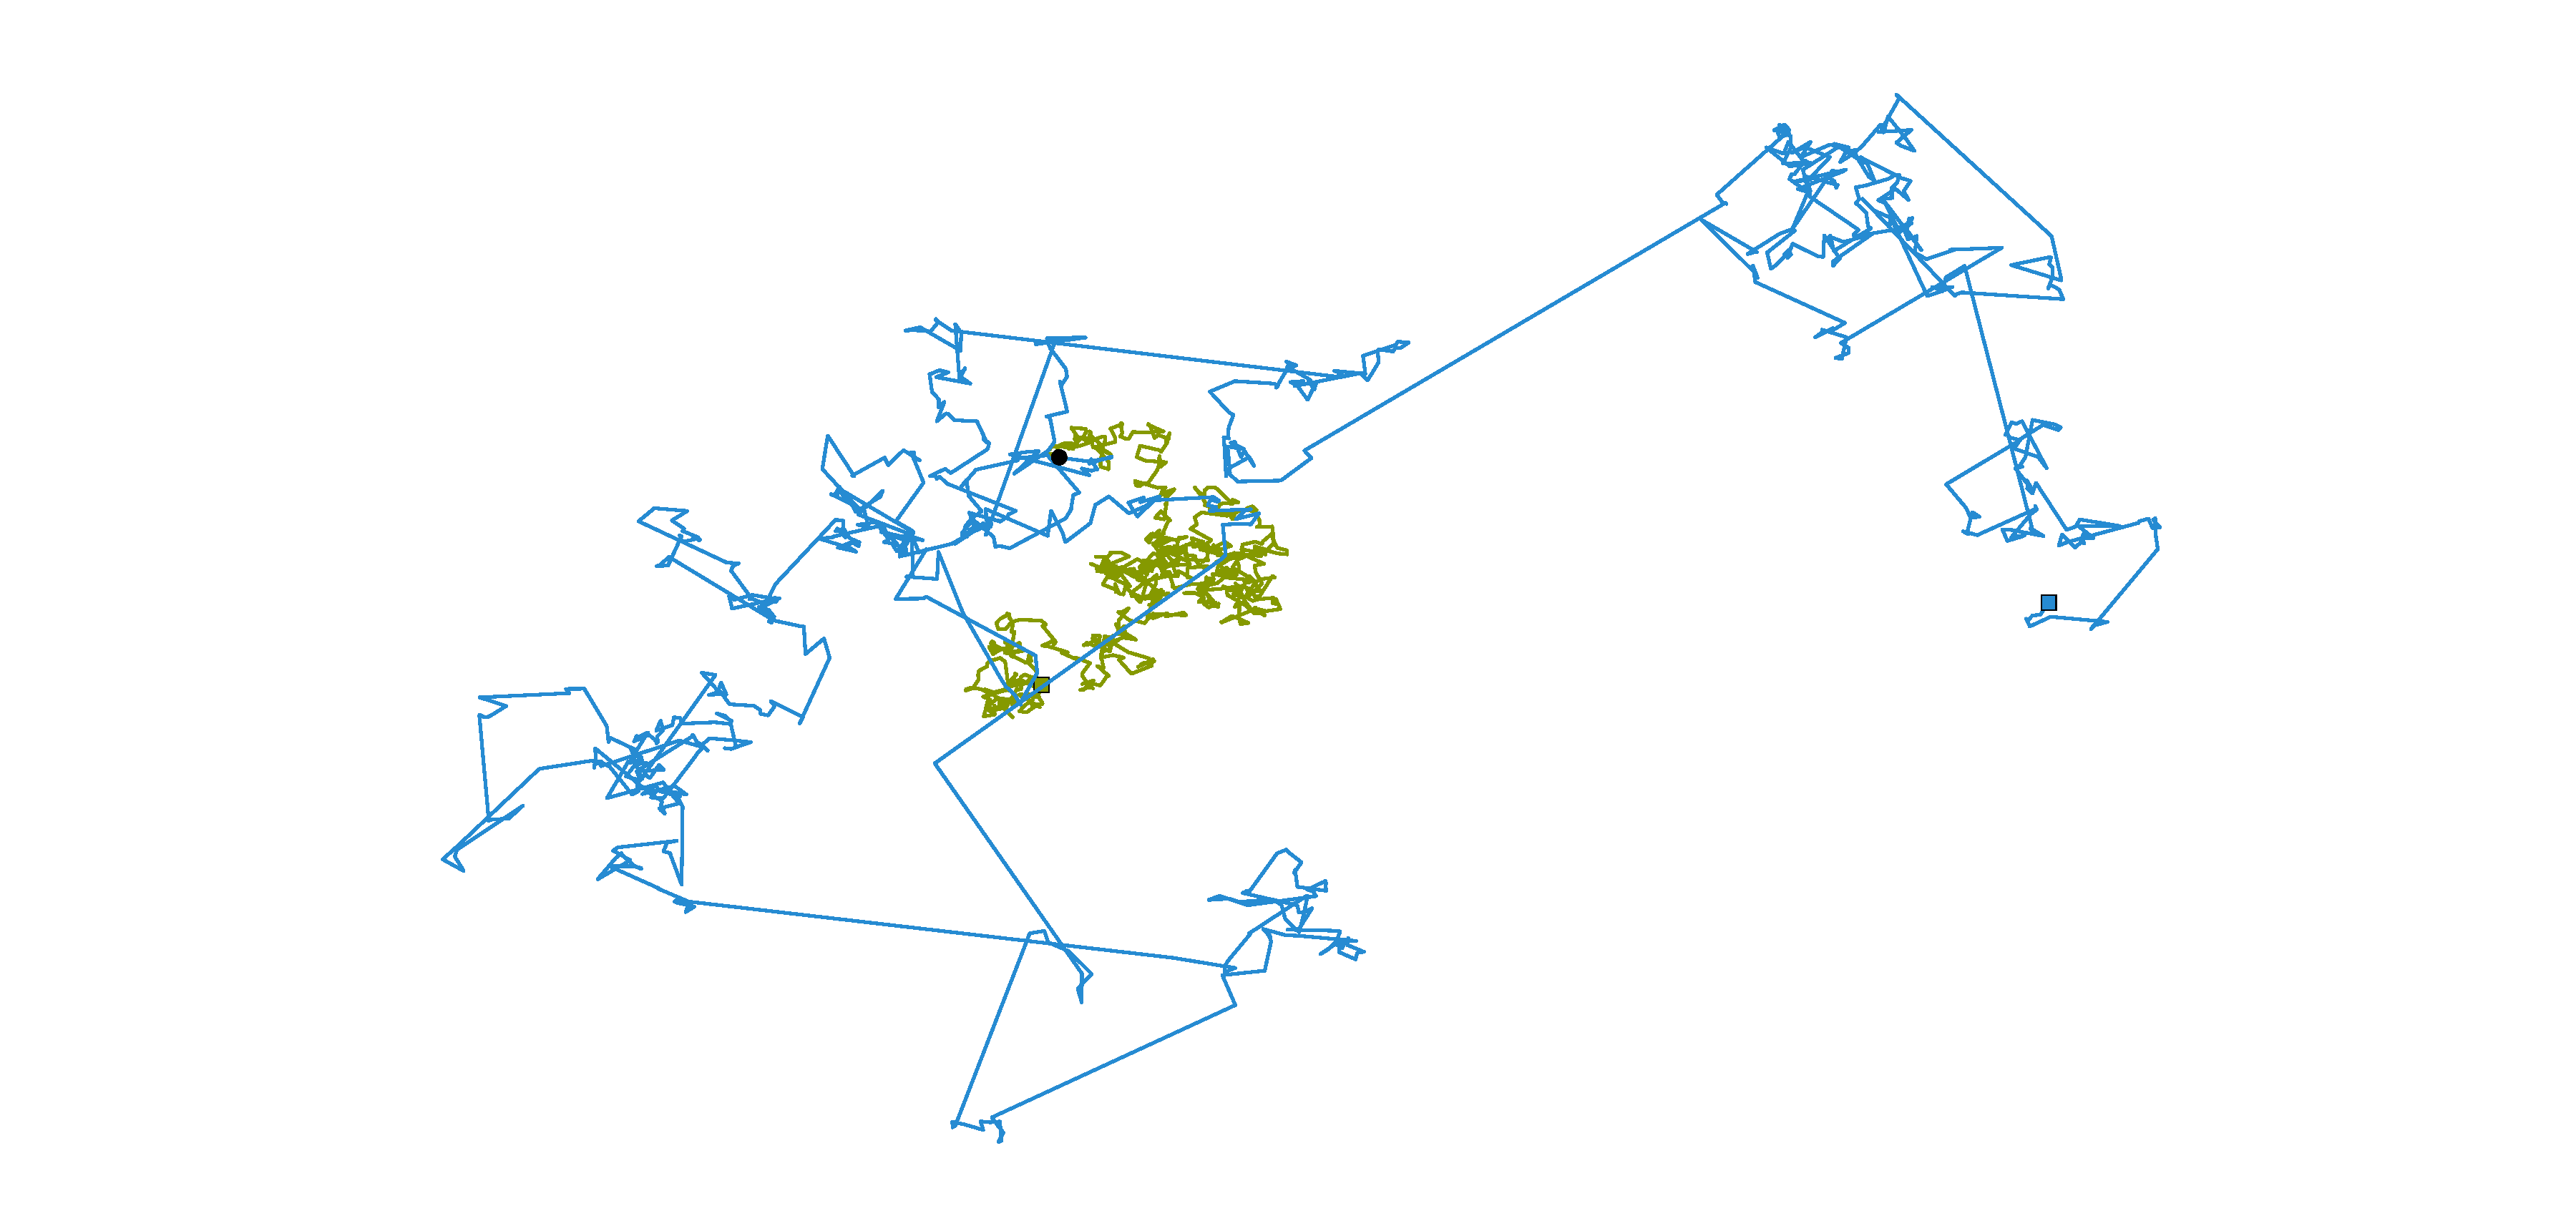
\includegraphics{Ressources/Images/LevyFlight/levy_vs_gaussian.pdf}
    \end{center}
    \caption{Mouvement brownien (en vert) et vol de Lévy (en bleu) pour 200 pas aléatoires.
             \label{fig:levy_vs_gaussian}}
\end{figure}
% subsection vol_de_levy (end)


% ------------------------------------------------------------------------------
\subsection{Apprentissage par vecteur opposé} % (fold)
\label{sub:apprentissage_par_vecteur_oppose}
Les méthodes d’optimisation et spécifiquement les méthodes approchées sont fortement
dépendantes de la population initiale (\mtodo{Ajouter source}). Il est ainsi nécessaire
de constituer une population couvrant de manière homogène l’espace de décision.
L’approche la plus répandue consiste à construire une population initiale stochastiquement
à l’aide d’une distribution uniforme suivant \eqref{alg:init_phase}.
Afin d’améliorer la diversité / qualité de la population initiale sans connaissance
a priori, \textcite{Tizhoosh2005695} a développé l’apprentissage par vecteur opposé
(\textit{OBL} pour Opposite Based Learning) (Définition~\ref{def:oblm}).

\begin{Def}[OBL~:~Apprentissage par vecteur opposé]\label{def:oblm}
Admettons une position de dimension $D$, $\vec{x}(x_{1}, x_{2}, ..., x_{D})$ avec
$x_{1}, x_{2}, ..., x_{D}$ des valeurs bornées. Si $x_{j} \in [c_{j}, d_{j}]$ pour
$j = 1, 2, ..., D$ alors la position opposée est $\vec{\check{x}}(\check{x_{1}},%
\check{x_{2}}, ..., \check{x_{D}})$ est définie par:
\[\check{x_{j}} = c_{j} + d_{j} - x_{j}\]
\end{Def}

\textcite{Rahnamayan2008906} l’adaptent pour l’algorithme Differential Evolution (\textit{DE})
et montrent que la probabilité d’améliorer une solution est plus grande si on sélectionne
la position opposée que si on tire aléatoirement une autre position.
Dans leur implémentation, ils l’utilisent durant l’initialisation mais aussi au cours du
processus d’optimisation. Les bornes ($c_{j}$ et $d_{j}$) sont alors définies dynamiquement
afin d’éviter de ralentir la convergence.
Cette approche a aussi été appliquée avec succès dans le cas de l’algorithme \textit{ABC}
en association avec un opérateur de mutation \parencite{Bi2011174}, ou encore en coopération
avec une marche aléatoire \parencite{Sharma2012213}. Elle a aussi été utilisée pour
résoudre des problèmes à objectifs multiples, en combinaison avec un algorithme
évolutionnaire \parencite{Ma201448}, ou encore avec le \textit{PSO} \parencite{Gao2013114}.

L’approche est ainsi retenue afin d’améliorer la diversité de la population initiale
et sera aussi utilisée durant la phase des exploratrices afin d’augmenter la qualité
de la nouvelle position.
Pour chaque source, une position candidate ($\vec{x}$) et son opposée
($\vec{\check{x}}$) sont ainsi évaluées. Une sélection par tournoi binaire permet
de retenir la meilleure des deux comme nouvelle position pour la source.
% subsection apprentissage_par_vecteur_oppose (end)


\subsection[L’epsilon-dominance]{L’$\epsilon$-dominance} % (fold)
\label{sub:l_epsilon_dominance}
Contrairement à une approche mono-objectif, il existe plusieurs solutions optimales
dans une approche multi-objectif. Il apparaît alors nécessaire de conserver l’évolution
du front de \textit{Pareto}~: c’est le rôle de l’archive \parencite{Laumanns2002263}.

Afin de garantir la convergence, il est nécessaire d’utiliser une approche élitiste
en limitant la population de l’archive aux solutions les plus performantes \parencite{Zitzler2000173}.
De plus, afin d’éviter de converger vers un front local, la population doit conserver
une bonne diversité.
L’algorithme de base du \textit{NSGA-II} \parencite{Deb2002182}, utilise le \textit{Fast
Non Dominated Sorting Algorithm} afin de construire son archive. Dans cette approche une
sélection par rang est appliquée afin de trier les solutions en différents niveaux et la
distance dite de crowding (distance moyenne entre deux solutions) est utilisée afin de
maintenir la diversité. L’algorithme \textit{SPEA II} cherche à améliore la diversité du
front final au prix d’une convergence plus lente en utilisant une approche par clustering.
Dans cette approche la taille limite de l’archive est définie par le nombre de cluster.
Ces clusters sont formés en se basant sur la distance euclidienne et une seule solution
est retenue.
\textcite{Laumanns2002263} proposent une autre approche, séparer l’espace des solutions en une
grille dont les dimensions sont définies par le vecteur $\vec{\epsilon}$. Dans cette
approche l’espace des objectifs est divisé en hypercubes, et chaque hypercube est comparé
selon l’$\epsilon$-dominance (Définition~\ref{def:eps_dominance}). Bien que d’autres
approches utilisent une grille similaire (PAES) \parencite{Knowles2000149},
l’$\epsilon$-dominance n’accepte qu’une unique solution par hypercube assurant une plus
grande diversité de la population. La taille de l’archive est donc fonction des $\epsilon$
choisis pour chaque objectif et est donc toujours garantie d’être finie.


\begin{Def}[$\epsilon$-dominance]\label{def:eps_dominance}
L’$\epsilon$-dominance assume que deux solutions sont identiques lorsqu’elles appartiennent
au même hypercube dont les dimensions des arrêtes sont définies par
$\vec{\epsilon}_{m}, m \in \{1, ..., M\}$ avec $M$ le nombre de fonctions objectif.
Dans le cas d’une maximisation il est dit que $\vec{x}_{a}$ $\epsilon$-domine $\vec{x}_{b}$ si~:
\begin{align*}
  \forall m \in \{1, M\}, \qquad
  \left\lceil\frac{f_{m}(\vec{x_{a}})}{\epsilon}\right\rceil &\leq
  \left\lceil\frac{f_{m}(\vec{x_{b}})}{\epsilon}\right\rceil  \\
  \intertext{et}
  \exists m \in \{1, M\}, \qquad
  \left\lceil\frac{f_{m}(\vec{x_{a}})}{\epsilon}\right\rceil &<
  \left\lceil\frac{f_{m}(\vec{x_{b}})}{\epsilon}\right\rceil  \\
\end{align*}
Cette relation sera notée~: $\vec{x}_{a} \prec_{\epsilon} \vec{x}_{b}$.
\end{Def}

Une solution peut ainsi être ou dominée, dominante, identique, ou non-dominée au sens de
l’$\epsilon$-dominance, les solutions $\epsilon$-non-dominées formant alors le front
d’$\epsilon$-Pareto (Fig.~\ref{fig:epsilon_dominance}). Lors de l’ajout d’une solution à
l’archive l’$\epsilon$-dominance est dans un premier temps utilisée afin de les
départager. Dans le cas où la nouvelle solution serait $\epsilon$-identique elle est
uniquement comparée avec celle déjà archivée dans le même hypercube. La distance
euclidienne est alors utilisée pour les départager. La solution retenue est celle la plus
proche de l’optimum de l’hypercube (coin supérieur droit dans le cas d’une maximisation).
Contrairement à une sélection par dominance stricte le calcul de la distance euclidienne
permet de tenir compte de l’ensemble des amélioration et est moins élitiste. Afin d’éviter
l’ajout de biais, les objectifs sont normalisés dans l’espace de l’hypercube.
L’$\epsilon$-archive permet ainsi d’assurer~:
\begin{itemize}
  \item L’élitisme~: seule les solutions non-dominées sont retenues
  \item La diversification~: une unique solution par hypercube
  \item Une taille limite~: La taille maximale est fonction de $\vec{\epsilon}$ et est finie
  \item Une intensification~: En réduisant $\vec{\epsilon}$ on augmente la taille maximale de l’archive
  \item Une réduction~: En augmentant $\vec{\epsilon}$ on réduit la taille maximale de l’archive
\end{itemize}

\begin{figure}
    \begin{center}
        \includegraphics{Ressources/Images/abc/selection_boxes.pdf}
    \end{center}
    \caption{Principe de la mise à jour de l’archive par epsilon-dominance (maximisation assumée).
             Adapté de \cite{Deb2005501}.
             \label{fig:epsilon_dominance}}
\end{figure}
L’étude réalisée par \textcite{Deb2005501} montre que l’$\epsilon$-dominance permet
d’obtenir une très bonne convergence et une grande diversité sur le front final.
Les résultats indiquent que les approches \textit{PESA} et \textit{NSGA II} obtiennent une moins
bonne représentation du front de Pareto que celles utilisant l’$\epsilon$-dominance
(\textit{$\epsilon$-MOEA}) ou le clustering (\textit{C-NSGA II}, \textit{SPEA}).
Cette observation est d’autant plus vraie pour des problèmes ayant plus de deux
objectifs (\textit{DTLZ1}, ..., \textit{DTLZ7}).
De plus les résultats mettent aussi en évidence que le \textit{NSGA II} et le \textit{$\epsilon$-MOEA}
convergent plus rapidement que le \textit{SPEA II}.
Un désavantage à cette méthode peut cependant être noté. De part sa formulation
les solutions au niveau des extrêmes sur le front de Pareto sont plus difficilement
atteignables.

L’$\epsilon$-archive est donc retenue comme solution d’archivage dans ces travaux
car il représente un bon compromis entre diversité et convergence.
% subsection l_epsilon_dominance (end)


% ------------------------------------------------------------------------------
\subsection{Tenir compte des contraintes} % (fold)
\label{sub:tenir_compte_des_contraintes}
Les problèmes multi-objectif dans le domaine de l’ingénierie sont souvent
dépendants de contraintes limitant l’ensemble des solutions optimales au domaine
de faisabilité. L’optimisation consiste alors à améliorer les objectifs tout en
respectant les contraintes spécifiques au problème \eqref{eq:def_optimisation}.

La littérature introduit de nombreuses méthodes permettant de tenir compte des
contraintes. L’approche la plus courante est d’utiliser un facteur de pénalité. Ce facteur
est dit statique si il est fixe durant l’ensemble de l’optimisation, dynamique si il est
adapté en fonction du nombre d’itérations, et adaptatif si les informations acquises par la
recherche aide à sa détermination \parencite{Coello2002}. Parmi les approches existantes il
peut être cité la méthode de la peine de mort. Elle consiste à appliquer une pénalité très
importante aux objectifs afin de rejeter toutes les solutions sous contraintes. Certaines
moins exclusives désavantagent les solutions ne respectant pas les contraintes en fonction
de leur niveau de violation alors que d’autres ajustent dynamiquement la pénalité en
fonction du nombre d’itérations déjà réalisées. Le problème récurrent avec ces approches
réside dans l’ajout de paramètres supplémentaires qui doivent être déterminés empiriquement.

\textcite{Coello2002} explique qu’une bonne prise en compte des contraintes ne devrait
pas nécessiter le paramétrage de facteurs car ils impactent
fortement la performance de la méthode. Finalement, la méthode sélectionnée ne
doit pas nécessiter un nombre plus important d’évaluations car elles peuvent être coûteuses.
\textcite{Deb2000311} propose une méthode de sélection par tournoi respectant ces conditions
dont les règles sont les suivantes~:
\begin{itemize}
  \item Une solution avec contraintes est inférieure à une solution sans contraintes
  \item Si les deux solutions sont sans contraintes la solution dominante est préférée
  \item Si les deux solutions sont sous contraintes, la solution violant le moins les contraintes est préférée
\end{itemize}
La méthode a l’avantage d’être simple à mettre en place mais est cependant
très élitiste car les solutions non faisables sont toujours écartées durant la
recherche.

Dans ces travaux, une méthode adaptative moins élitiste est retenue. Adaptée
aux problèmes multi-objectif par \textcite{Woldesenbet20073077}, la méthode ne demande
aucun paramétrage, et l’objectif modifié est calculé de la manière suivante~:
\begin{itemize}
  \item Normaliser les objectifs selon \eqref{eq:norm_obj}
  \item Normaliser les contraintes et les agréger pour former une unique contrainte selon \eqref{eq:norm_contrainte}
  \item Calculer les objectifs modifiés par agrégation des contraintes et des objectifs selon \eqref{eq:calc_modif_obj}
\end{itemize}

\begin{align}\label{eq:norm_obj}
  \tilde{f}_{m}(\vec{x}) &= \begin{cases}
    \frac{f_{m}(\vec{x}) - min(f_{m}(\vec{x}))}{max(f_{m}(\vec{x})) - min(f_{m}(\vec{x}))}
    & \text{(minimisation)} \\ \\ 1 - \left[\frac{f_{m}(\vec{x}) -
    min(f_{m}(\vec{x}))}{max(f_{m}(\vec{x})) - min(f_{m}(\vec{x}))}\right] &
    \text{(maximisation)} \\
  \end{cases}
\end{align}
avec $f_{m}(\vec{x})$ la valeur de l’objectif $m$, pour la position $\vec{x}$ dans l’espace de décision.

\begin{equation}\label{eq:norm_contrainte}
  v(\vec{x}) = \frac{1}{Q} \sum_{q=1}^{Q} \left(\frac{g_{q}(\vec{x})}{max(g_{q}(\vec{x}))}\right)
\end{equation}
avec $Q$ le nombre de contraintes d’inégalités. $g_{q}$ représente alors la fonction contrainte
associée à la contrainte $q$ avec $g_{q} \geq 0$. Dans cette représentation les contraintes
d’égalité doivent être transformées en contraintes d’inégalité.

\begin{equation}\label{eq:calc_modif_obj}
  F_{m}(\vec{x}) = d_{m}(\vec{x}) + p_{m}(\vec{x})
\end{equation}
avec $d_{m}(\vec{x})$ calculée selon \eqref{eq:dist_obj} et $ p_{m}(\vec{x})$ selon \eqref{eq:penalty_norm}.


\begin{align}\label{eq:dist_obj}
  d_{m}(\vec{x}) = \begin{cases}
                          v(\vec{x})                                     & \qquad si\  r_{f} = 0 \\
                          \sqrt{v(\vec{x})^2 + \tilde{f}_{m}(\vec{x})^2} & \qquad sinon          \\
                    \end{cases}
\end{align}
\begin{equation}\label{eq:penalty_norm}
  p_{m}(\vec{x}) = (1 - r_{f})  X(\vec{x}) + r_{f} Y_{m}(\vec{x}) \\
\end{equation}

\begin{align*}
  \shortintertext{où} \\
    r_{f} &= \frac{\text{Nombre de solutions réalisables}}{\text{Taille de la population}} \\
  \shortintertext{et} \\
  X(\vec{x})     &= \begin{cases}
                0,          \qquad     & si\  r_{f} = 0\\
                v(\vec{x}), \qquad     & sinon\\
                \end{cases} \\
  Y_{m}(\vec{x}) &= \begin{cases}
                    0,          \quad \qquad & \text{si} \ \forall q, \ g_{q}(\vec{x}) = 0\\
                      \tilde{f}_{m}(\vec{x})  \\
            \end{cases}\\
\end{align*}

L’algorithme s’adapte ainsi dynamiquement à la population et peut accepter des
solutions ne respectant pas les contraintes. Plus il y a de solutions non
réalisables dans la population, moins une solution ne respectant pas les contraintes à
de chances d’être sélectionnée. L’approche permet d’améliorer l’exploration de
l’espace de décision et ainsi de pouvoir trouver des solutions existantes même
lorsque l’espace de faisabilité est faible.
L’approche est donc retenue dans ces travaux afin de mettre à jour la position des
sources, les solutions retenues dans l’archive doivent elles respecter
l’ensemble des contraintes pour être acceptées.
% subsection tenir_compte_des_contraintes (end)


% ------------------------------------------------------------------------------
\subsection{Description de l’approche globale} % (fold)
\label{sub:description_de_l_approche_globale}
Dans la section précédente, chaque élément utilisé dans l’algorithme a été détaillé et
les avantages et inconvénients des approches retenues ont aussi été explicités.
Dans cette section le fonctionnement global de la méthode approchée d’optimisation
multi-objectif retenue est décrit.

L’algorithme peut être défini par Fig.~\ref{fig:abc_complet} et le détail de chaque
phase est décrit à travers ci-après.
Les sources sont initialisées (Algorithm~\ref{alg:init_phase}) suivant la méthode
\textit{OBL} (Définition~\ref{def:oblm}) afin d’obtenir une meilleure représentation du
domaine de décision en amont de l’optimisation.
Durant la phase des butineuses (Algorithm~\ref{alg:employed_phase}), chaque source
subit une variation en tenant compte de deux sources, une de l’essaim et une de l’archive.
Durant la phase des ouvrières (Algorithm~\ref{alg:onlooker_phase}), la qualité de
chaque source \eqref{eq:attribution_prob_to_source} est utilisée afin de sélectionner
et d’exploiter seulement les plus prometteuses. Finalement, si une source a été
modifiée infructueusement plus de $MaxEchec$, alors une exploratrice
réinitialise sa position de manière aléatoire  (Algorithm~\ref{alg:scout_phase}).
Tant que la condition d’arrêt n’est pas atteinte, les phases des butineuses,
des ouvrières, et des exploratrices sont répétées de manière cyclique. Au cours de
la recherche les nouvelles sources sont ajoutées à l’archive et sont utilisées
comme élément d’apprentissage pour les abeilles butineuses ou ouvrières. Les
exploratrices, elles, n’utilisent jamais d’éléments sociaux d’apprentissage.
Finalement, une fois la condition d’arrêt atteinte l’ensemble des solutions
de l’archive forme le front de Pareto.

\begin{figure}
    \begin{center}
        \includegraphics[width=10cm]{Ressources/Images/abc/algorithme_complet.pdf}
    \end{center}
    \caption{Description globale de l’algorithme ABC pour les problèmes multi-objectif.
             \label{fig:abc_complet}}
\end{figure}

Dans l’optique de l’optimisation d’un modèle solaire développé sous \textit{Dymola}, l’algorithme
a été implémenté en \textit{Python} afin de faciliter le couplage avec la bibliothèque
\textit{BuildingsPy} qui comme nous l’avons vu dans le chapitre précédent permet d’automatiser
la simulation de modèle \textit{Modelica} sous \textit{Dymola}. La bibliothèque est
disponible sous le nom de \textit{pyMOABC} et implémente~:
\begin{itemize}
  \item Une $\epsilon$-archive et la hypercube-dominance
  \item La dominance au sens de Pareto
  \item La prise en compte des contraintes suivant la méthode de \textcite{Woldesenbet20073077}
  \item Une interface commune permettant l’abstraction du type de variable (discrète, continue, qualitative)
  \item Une représentation des solutions (sources et abeilles)
  \item L’algorithme tel que décrit dans ces travaux
  \item Une suite de test unitaires et des cas théoriques validant l’approche avec
        et sans contraintes
\end{itemize}

L’approche retenue contrairement à la majorité des méta-heuristiques demande
peu de paramètres à définir de manière empirique et est ainsi robuste. En effet
seule la taille de la population $NP$, et le nombre d’essais maximum $MaxEchec$ sont à définir.
De plus la taille de la population n’impacte pas le nombre de solutions dans l’archive
car le stockage est réalisé dans une structure indépendante. Il est aussi important
de noter que les deux uniques paramètres ont un comportement prévisible facilitant
leur paramétrage. La taille de la population en augmentant améliore l’exploration
réduisant les risques de stagner vers des optimums locaux mais réduit la vitesse
de convergence (Définition~\ref{def:convergence}).
Le nombre d’essais maximum lui est directement lié au nombre de variables de décision
et à la taille de la population. Une valeur faible se traduit par un abandon rapide
des solutions alors qu’une valeur plus grande augmente le nombre de variations évaluées
pour chaque source. Ainsi on note clairement l’impact de chaque paramètre sur la
performance de l’algorithme simplifiant sa paramétrisation.

% Phase d’initialisation
\begin{algorithm}\label{alg:init_phase}
  \SetAlgoVlined
  \DontPrintSemicolon
  \emph{Initialisation des \ASources sur l’ensemble de l’espace de décision}\;
  \For{$i \leftarrow 0$ \KwTo \ANbrSources}
  {
    \emph{Initialisation des variables de décision pour chaque source}\;
    \For{$j \leftarrow 0$ \KwTo \ANbrVariables}
    {
      \encircle{a} \emph{Initialisation de la position de la $\ASource_{i}$ de manière aléatoire}\;
      \Indp
      $x_{ij} = x_{j}^{min} + RandUniform(0, 1) \times (x_{j}^{max} - x_{j}^{min})$\;
      \Indm
      \BlankLine
      \encircle{b}  \emph{Génération de l’$\ABee_{i}$ dont la position est calculée suivant Définition~\ref{def:oblm}}\;
      \Indp
      $ \check{x_{ij}} = x_{j}^{min} + x_{j}^{max} - x_{ij}$\;
      \Indm
      \BlankLine
      \encircle{c} \emph{Évaluation de la $\ASource_{i}$ et de l’$\ABee_{i}$}\;
      \BlankLine
      avec $RandUniform$ un tirage aléatoire suivant une loi uniforme, et $x_{j}^{min}$, $x_{j}^{max}$
      respectivement le minimum et le maximum de la variable $j$\;
    }
    \If{$\ASource_{i}$ respecte toutes les contraintes}
    {
      $\AArchive \pluseq \ASource_{i}$ \AComment{On ajoute la source initial à l’archive}
    }
    \If{$\ABee_{i}$ respecte toutes les contraintes}
    {
      $\AArchive \pluseq \ABee_{i}$ \AComment{On ajoute la source opposée à l’archive}
    }
  }
  Mise à jour des \ASources d’après Algorithm~\ref{alg:maj_phase}\;
  \caption{Initialisation des sources par OBLM (Définition~\ref{def:oblm}).}
\end{algorithm}

% Phase des éclaireuses
\begin{algorithm}\label{alg:scout_phase}
  \SetAlgoVlined
  \DontPrintSemicolon
  \AComment{Exploration par les \AScouts}
  \For{$i \leftarrow 0$ \KwTo \ANbrSources}
  {
    \If{$\ATrial_{i} > \AMaxTrial$ }
    {
      Génération de deux nouvelles positions suivant Algorithm~\ref{alg:init_phase}\;
    }
  }
  Mise à jour de la position des \ASources d’après Algorithm~\ref{alg:maj_phase}\;
  \caption{Phase des éclaireuses.}
\end{algorithm}


% Phase des ouvrières
\begin{algorithm}\label{alg:onlooker_phase}
  \SetAlgoVlined
  \DontPrintSemicolon
  \AComment{Exploitation des sources par les \AOnlookers}
  \AComment{Plusieurs \AOnlookers peuvent modifier la même source}
  \For{$\AOuvriere \in \AOnlookers$}
    {
      Sélection aléatoire d’une \ASource $i$ selon la probabilité
      définie par l’équation \eqref{eq:attribution_prob_to_source}\;
      Sélection aléatoire d’une source $a$ ($a \neq i$) dans l’\AArchive\;
      \encircle{a} \emph{Génération d’une nouvelle position $\vec{x_{i}}'$ à partir de la
                         position $\vec{x_{i}}$ pour l’\AOuvriere }\;
      \For{$j \leftarrow 0$ \KwTo \ANbrVariables}
      {
      \begin{algomathdisplay}
        x_{ij}' =%
          \begin{cases}
            x_{ij}  + RandUniform(-1, 1)   \times \ (x_{ij} - x_{aj}) &\ \ATirageB < \AMR \\
            x_{ij}                                                    &\ sinon
          \end{cases}
      \end{algomathdisplay}
      }
      \BlankLine
      Avec \AMR est la probabilité de réaliser une modification (fixée à 0,2) et
      \ATirageB un nombre aléatoire entre 0 et 1\;
      \BlankLine
      \encircle{b} \emph{Évaluation des objectifs pour la nouvelle position $\vec{x_{i}}'$}\;
      \BlankLine
      \If{\AOuvriere respecte toutes les contraintes}
      {
        $\AArchive \pluseq \AOuvriere$ \AComment{Ajout de la solution trouvée par l’\AOuvriere à l’archive}
      }
    }

  Mise à jour de la position des \ASources qui ont été modifiées d’après Algorithme~\ref{alg:maj_phase}\;
  \caption{Phase des ouvrières.}
\end{algorithm}

% Maj des sources
\begin{algorithm}\label{alg:maj_phase}
  \SetAlgoVlined
  \DontPrintSemicolon
  Récupérer le maximum et minimum pour chaque objectif dans l’\AHive\;
  Récupérer le maximum pour chaque contrainte dans l’\AHive\;
  \For{$\ABee \in \ABees$}
  {
    Calcul du vecteur objectif pour l’\ABee ($\vec{F}'_{i}$) et pour sa \ASource $i$ ($\vec{F}_{i}$),
    respectivement aux positions $\vec{x_{i}}'$ et $\vec{x_{i}}$
    selon \eqref{eq:calc_modif_obj}\;
    \For{$m \leftarrow 1$ \KwTo M}
    {
      \begin{algomathdisplay}
      \begin{aligned}
      F_{im}' &= d_{m}'(\vec{x_{i}}) + p_{m}'(\vec{x_{i}}) \\
      F_{im}  &= d_{m}(\vec{x_{i}}) + p_{m}(\vec{x_{i}})   \\
      \end{aligned}
      \end{algomathdisplay}
    }
    \If{$\vec{x_{i}}' \succ \vec{x_{i}}$}
    {

      $\ASource_{i} \leftarrow \ABee$ \AComment{Mise à jour de la \ASource à partir de l’\ABee}

      $\ATrial_{i} \leftarrow 0$ \AComment{On réinitialise le nombre d’essais pour la \ASource $i$}
    }
    \Else
    {
      $\ATrial_{i} \pluseq 1$ \AComment{On incrémente le nombre d’essais pour la \ASource $i$}
    }
  }
  \caption{Mise à jour des \textbf{Sources} par les \textbf{Abeilles}}
\end{algorithm}

% Phase des butineuses
\begin{algorithm}\label{alg:employed_phase}
  \SetAlgoVlined
  \DontPrintSemicolon
  \AComment{Exploration des sources par les \AEmployed}
  \For{$i \leftarrow 0$ \KwTo \ANbrSources}
  {
    Sélection aléatoire d’une source $a$ ($a \neq i$) dans l’\AArchive\;
    Sélection aléatoire d’une source $b$ ($b \neq i$) dans l’\AHive\;
    \BlankLine
    \encircle{a} \emph{Génération d’une nouvelle position $\vec{x_{i}}'$ à partir de la %
                       position $\vec{x_{i}}$ pour la \AButineuse $i$}\;
    \If{$\ATirageA < \ARatio $ }
      {
      \For{$j \leftarrow 0$ \KwTo \ANbrVariables}
      {
      \begin{algomathdisplay}
        x_{ij}' =%
          \begin{cases}
            \begin{aligned}
              x_{ij}  &+ 0.01 \times ~\ALevy  &\times (x_{ij} - x_{bj})  \\
                      &+ 0.01 \times |\ALevy|   &\times (x_{aj} - x_{ij})  \\
            \end{aligned} &\ \ATirageB < \AMR \\
            x_{ij}        &\ sinon
          \end{cases}
      \end{algomathdisplay}
      \ALevy est nombre aléatoire dans une distribution de Lévy
      permettant de réaliser un vol de Lévy (Définition~\ref{def:vol_levy})\;
      }
      }
    \Else
      {
      \For{$j \leftarrow 0$ \KwTo \ANbrVariables}
      {
      \begin{algomathdisplay}
        x_{ij}' =%
          \begin{cases}
            \begin{aligned}
              x_{ij}  &+ RandUniform(-1, 1)   &\times \ (x_{ij} - x_{bj})  \\
                      &+ RandUniform(0, 1)    &\times \ (x_{aj} - x_{ij})  \\
            \end{aligned} &\ \ATirageB < \AMR \\
            x_{ij}        &\ sinon
          \end{cases}
      \end{algomathdisplay}
      }
      }
      Où \ARatio est la probabilité de réaliser un vol de Lévy (fixée à 0,5), et \AMR la probabilité
      de réaliser une modification (fixée à 0,3). \ATirageA et \ATirageB étant des nombres aléatoires
      (entre 0 et 1) tirés dans une distribution uniforme\;
      \BlankLine
    \encircle{b} \emph{Évaluation des objectifs pour la nouvelle position $\vec{x_{i}}'$}\;
    \If{$\AButineuse_{i}$ respecte toutes les contraintes}
    {
      \AComment{On ajoute la nouvelle source à l’archive}
      $\AArchive \pluseq \AButineuse_{i}$\;
    }
  }
  \AComment{On ne conserve qu’une seule position par source}
  Mise à jour de la position des \ASources d’après Algorithme~\ref{alg:maj_phase}\;
  \caption{Phase des butineuses.}
\end{algorithm}
% subsection description_de_l_approche_globale (end)


% ------------------------------------------------------------------------------
\subsection{Validation de la méthode} % (fold)
\label{sub:validation_de_la_methode}

\itodo{CETTE SECTION EST EN CONSTRUCTION}

Cette section permet d’apprécier la performance de l’approche pour différentes types
de problèmes pouvant être rencontrés dans un problème d’optimisation.

La bibliothèque \textit{pyMOABC} a été développée autour de tests unitaires
(Test-driven development).
Chaque éléments (fonction / méthodes / ...) et comportements (minimisation / maximisation / ...)
ont ainsi été testés afin de garantir que la bibliothèque implémente correctement
les éléments et comportements nécessaires. De part son approche, chaque nouvelle
modification tient implicitement compte des tests précédents et garantie ainsi
l’intégrité du code lors de son développement.
L’algorithme et les briques nécessaires implémentés, des problèmes étalons ont été
utilisés afin de valider la performance de l’approche. Bien que la réussite d’un
problème étalon ne soit pas une condition suffisante pour garantir la convergence
sur un problème réel, il apporte une information importante~: la capacité de
l’algorithme à s’adapter aux différents types de contraintes pouvant survenir.

Dans cette optique les résultats présentés dans cette section sont sélectionnés
afin de couvrir les principales difficultés existantes~:
\begin{itemize}
  \item front convexe~: ZDT1 (2 objectifs)
  \item front linéaire~: Hanne 1 (2 objectifs)
  \item front concave~: ZDT2 (2 objectifs)
  \item multi-modal~: ZDT4 (2 objectifs)
  \item Non-uniformité avec faible densité près de l’optimal~: DTLZ5 (3 objectifs), ZDT6, ConvexGlobalNonConvexLocalHive
  \item Discontinue~: DTLZ6 (3 objectifs), Kursawe
\end{itemize}
La validation portera ainsi sur la capacité de l’algorithme à converger vers le
front de Pareto ainsi que la qualité des solutions obtenues à travers l’évaluation
de sa diversité. De plus la vitesse de convergence vers le front sera aussi discutée.
Concernant la méthode de prise en compte des contraintes, des travaux ont déjà
évalué sa performance et ces résultats ne seront pas repris dans cette section (\mtodo{Ajouter ref}).

\itodo{Ajout de graphe de convergence, et les résultats du calcul des indicateurs
       évaluant la diversité, la rapidité, et la convergence.}
% subsection validation_de_la_methode (end)
% section algorithme_de_colonie_d_abeilles_virtuelles (end)


\chapter{Optimisation d’un système solaire combiné}
% Chap4-OptimisationSystemeSolaire

\section{Construction d’un système solaire: Un problème d’optimisation multicritère} % (fold)
\label{sec:construction_d_un_systeme_solaire_un_probleme_d_optimisation}
% -----------------------------------
% Rappeler ce qui différencie cette approche des autres issues de la littérature:
%  - Approche couplée système/enveloppe
%  - Optimisation complète systèmes/contrôle/enveloppe

% Aide à la décision nécessite en set de solutions optimales:
%  - Génération d’un jeu de solutions optimales

L’optimisation multi-critère est aujourd’hui largement utilisé dans le bâtiment.
On a par exemple \cite{Armand-Decker2015} qui a développé une méthode d’optimisation pour les
construction bois en utilisant un meta-modèle de bâtiment. Elle utilise un meta-heuristique

à population (Particule Swarm optimization) et évalue les besoins en énergie, le confort des
occupants, la sécurité de l’ouvrage et de l’impact environnemental. \cite{Rivallain2013}
a quand à lui utilisé une méthode approchée (NSGA-II) et une exacte (programmation dynamique)
pour identifier des programmes séquentiels efficaces de réhabilitation énergétique.
Il a ainsi optimisé la combinaison des modifications pour chaque phase mais aussi l’ordre
dans lequel ces améliorations doivent être réalisées afin d’être le plus optimal
possible.
Pour les différentes solutions l’impact environnemental, le confort des occupants en
période estivale, et le coût ont été évaluées.
\itodo{Ajouter des sources vers des exemples d’optimisation de bâtiment}


On a aussi de nombreux exemples d’optimisation de système énergétique.
\itodo{Ajouter des sources vers des exemples d’optimisation de système}

On voit donc que l’optimisation est un outil qui a été largement utilisé dans
le bâtiment comme pour l’amélioration ou l’identification de solutions performantes
pour les systèmes.
L’originalité de ce travail provient principalement du couplage entre le bâtiment
et ses systèmes. La plupart des optimisations de bâtiment évalues les besoins
du bâtiment et considère donc un système de chauffage et de ventilation idéaux.
Dans ces travaux on cherche à optimiser la partie système et son algorithme de
contrôle en même temps que l’enveloppe du bâtiment. On évalue donc plus un besoin
en énergie mais une consommation qui est fonction de la performance des systèmes
envisagées. Les travaux se concentre sur l’évaluation de solutions utilisant fortement
l’énergie solaire comme vecteur énergétique. On cherche donc à couvrir les besoins
de chauffage, d’eau chaude sanitaire (ECS) et d’électricité.
Cette approche permettra d’évaluer le potentiel d’autonomie solaire disponible
pour différentes combinaisons systèmes/enveloppe.
\itodo{Ajouter du bla bla sur l’originalité et les perspectives de ces travaux}

Enfin ces travaux vise à l’élaboration d’un outil d’aide à la décision. Il existe
diverses methodes pour faire de l’aide à la décision comme décrites dans le chapitre
précédent~\autoref{sec:multi_critere}. L’approche choisie est de déterminer un
ensemble de solutions non-dominées dans un premier temps, puis d’utiliser des
outils d’aide à la décision pour réduire le nombre de solution. On se trouve donc
dans une approche par front de Pareto.
\itodo{Ajouter du bla bla sur le choix de l’ordre entre optimisation et aide à la décision}


Dans les sections suivantes nous décrirons dans un premier temps les hypothèses
retenues pour l’étude. Dans un second temps nous décrirons le processus retenu
pour l’outil d’aide à la décision.

\itodo{Reformuler tout ça pour mieux introduire les parties qui suivent}

% section construction_d_un_systeme_solaire_un_probleme_d_optimisation (end)




\section{Cas d’étude: Un système solaire combiné couplée à une maison passive} % (fold)
\label{sec:cas_d_etude_un_systeme_solaire_combine_couplee_a_une_maison_passive}
% -----------------------------------
\subsection{Hypothèses retenues} % (fold)
\label{sub:hypotheses_retenues}
\subsubsection{Description du site étudié} % (fold)
\label{ssub:description_du_site_etudie}
% Description du site étudié:
%  - Climat
%  - Données météos
%  - ...
Afin d’évaluer et d’optimiser la performance d’un système solaire, il est nécessaire
que les conditions extérieures ne soit pas fortement favorable.
Les climats méditerranéens ne sont donc pas des cas d’étude intéressant du fait
de la forte couverture solaire.
À l’opposé le climat de Limoges est assez rude et l’ensoleillement durant la période
hivernale est faible. C’est donc un cas d’étude intéressant.
\itodo{Ajouter une carte pour localiser la ville}
\itodo{Ajouter une description plus complète avec DJU, extrèmes, ...}
\itodo{Refaire complètement ce paragraphe car il fait pitié actuellement}
% subsubsection description_du_site_etudie (end)


\subsubsection{Description de la maison etudiée} % (fold)
\label{ssub:description_de_la_maison_etudiee}
% Description de la maison:
%  - Composition de base
%  - Surface
%  - ...
La maison fait 100\,\si{m^{2}} est est composée de ...
\itodo{Ajouter du bla bla sur la composition de la maison}
% subsubsection description_de_la_maison_etudiee (end)


\subsubsection{Description des scénarios} % (fold)
\label{ssub:description_des_scenarios}
% Descriptions des paramètres fixes:
%  - L’occupation
%  - La température de consigne
%  - Charges internes
%  - ...
Le cas d’étude utilise les scénarios d’une famille moyenne développés au travers de
la création d’un outil pour évaluer l’impact des occupants sur les besoins
énergétiques du bâtiment (\cite{Vorger2014}).
\itodo{Décrire rapidement les travaux d’Éric}

Pour cette étude différents scénarios ont été pris en compte de manière fixe:
\begin{itemize}
    \item Occupation
    \item Charges internes (faibles par rapport à un scénario RT)
    \item Température de consigne
    \item Débits d’extractions d’air
\end{itemize}
\itodo{Décrire les différents scénarios avec des illustrations}

D’autres font partis intégrante de l’optimisation. En effet ils influencent le
fonctionnement du système et donc sa performance. Les scénarios non-fixes sont donc
les suivants:
\begin{itemize}
    \item Occupation
    \item Profil de puisage ECS
    \item Température de consigne solaire
\end{itemize}
\itodo{Décrire les scénarios variables}
% subsubsection description_des_scenarios (end)
% subsection hypotheses_retenues (end)
% section cas_d_etude_un_systeme_solaire_combine_couplee_a_une_maison_passive (end)



\section{Formulation du problème d’optimisation} % (fold)
\label{sec:formulation_du_probleme_d_optimisation}
% -----------------------------------
\subsection{Définition des objectifs et contraintes} % (fold)
\label{sub:definition_des_objectifs_et_contraintes}
\subsubsection{Les objectifs de l’étude} % (fold)
\label{ssub:les_objectifs_de_l_etude}
% Définition des objectifs:
%  - Couverture solaire chauffage
%  - Couverture solaire ECS
%  - Coût de l’installation
%  - Temps de retour sur investissement
Dans cette étude on considère trois fonctions objectifs. On cherche dans un premier
temps à évaluer la performance du système solaire. Pour ce faire on évalue sa
performance sur le chauffage et sur la production d’ECS séparément. Il en a enfin
été noté dans ~\autoref{sec:approche_monozone} que certaines variations impactent
de manière différentes la part de chauffage et d’ECS. Enfin on a vu dans
~\autoref{sub:description_des_systemes} que la production d’ECS reste prioritaire
sur le chauffage, la modification du profil de puisage aura donc un impact différent
sur le chauffage et l’ECS.
\itodo{Il est aussi nécessaire de mettre en valeur l’impact de l’algorithme sur
      les rendements}

Le dernier objectif qui sera pris en compte est l’\textbf{impact économique}. Il
est important de ne pas seulement se focaliser sur la performance du système afin
de filtrer les solutions certes très performantes mais non-réalisable dans les années
proches. Il est ainsi important de rappeler que ces travaux se focalise sur une
technologie innovante mais pouvant être implémentées aujourd’hui.
Ainsi ce facteur bien que discutable du fait de son caractère changeant est indispensable
dans notre étude pour guider la recherche et donner un ordre de prix pour une solution
type.
L’optimisation se portera ainsi sur la maximisation de la couverture solaire pour
(i) le chauffage, (ii) la production d’eau chaude sanitaire, et la minimisation
du coût d’installation et du temps de retour sur investissement.
\itodo{Décrire les différents objectifs retenues avec plus de bla bla}
% subsubsection les_objectifs_de_l_etude (end)


\subsubsection{Les contraintes de l’étude} % (fold)
\label{ssub:les_contraintes_de_l_etude}
% Définition des contraintes:
%  - Surface de toiture à partager (Photovoltaïque)
%  - Équilibre entre production/consommation (Primaire)
Les objectifs sont maintenant clairement définies mais l’étude comporte plusieurs
contraintes qui doivent être prises en compte durant le processus d’optimisation.
La première contrainte est la surface de toiture qui est limitée et doit donc être
partagée entre les panneaux photovoltaïques et thermiques. Comme nous l’avons définie
(~\autoref{sub:description_des_systemes}) le cas d’étude étudié comporte des pans
de toiture avec diverses orientations ce qui complète la première contrainte.
On a donc une double contrainte, à savoir
partager la surface de toiture pour chaque orientation entre les différents capteurs.
Des études ont déjà été réalisées pour évaluer le meilleur ratio entre photovoltaïque
et thermique\mtodo{Ajouter citation} mais traite le problème sans tenir compte des combinaisons
entre les équipements, la structure, la régulation, ... Ces travaux permettront donc
d’obtenir plus d’informations sur cet aspect encore aujourd’hui faiblement exploré.
\itodo{Retrouver la publication qui parle de ratio thermique/photovoltaïque}

La seconde contrainte est la place disponible dans la maison pour accueillir les
équipements.
\itodo{Bla bla bla}

Enfin la contrainte principale est sur l’équilibre entre production et consommation
d’énergie primaire. En effet l’approche MEPOS ou encore NZEB définit comme requit
pour une maison passive d’avoir un équilibre entre production et consommation.
On a donc ici une contrainte forte au niveau énergétique.
\itodo{Bla bla bla}
\itodo{Décrire les contraintes et la méthode utilisée pour les traiter}
% subsubsection les_contraintes_de_l_etude (end)
% subsection definition_des_objectifs_et_contraintes (end)
% section formulation_du_probleme_d_optimisation (end)


\subsection{Choix des variables de décision} % (fold)
\label{sub:choix_des_variables_de_decision}
% Choix des variables de décisions:
%  - Propre au bâtiment
%  - Propre au système
%  - Propre au contrôle
Dans cette partie sera décrit les différentes variables qui ont été sélectionnées
en amont du **screening**.
\itodo{Décrire l’ensemble des variables considérées en amont de l’étude de sensibilité
      classée par groupe, système, contrôle, enveloppe, scénarios}
% Définir chaque variable:
%  - Type
%  - Plage de variation
%  - Unité
%  - Description
\itodo{Dresser une liste des caractéristiques de chaque critère}
\itodo{Faire apparaître clairement (graphiquement) l’impact de chaque variables
      sur les différents objectifs peut être pas à mettre ici mais plus dans
      ~\autoref{sub:reduction_de_la_cardinalite_par_screening}}
% subsection choix_des_variables_de_decision (end)




\section{Méthode retenue pour le dimensionnement du système} % (fold)
\label{sec:methode_retenue_pour_le_dimensionnement_du_systeme}
% -----------------------------------
Comme nous l’avons vu précédemment, il existe de nombreux meta-heuristiques dans
la littérature. Cependant il n’existe pas à la connaissance de l’auteur de méthode
pour sélectionner un algorithme qui sera le plus performant pour un problème donnée.
Ce principe a été formalisé par \cite{Wolpert199767} \itodo{Pas encore lu ...}. Il démontre qu’il
n’y a aucunes \emph{à priori} différences entre les algorithmes. Les critères
permettant de sélectionner un meta-heuristique sont donc à caractère subjectif.
Un des arguments pertinent qui peut être mis en avant est le nombre de paramètres
nécessaires pour le réglage de l’algorithme. En effet sur ce point les algorithmes
sont très différents, certains demandant de nombreux paramètres à configurer
\itodo{Citer des exemple de algo génétique, réseaux de neuronnes, ...} contrairement
à d’autres \itodo{Citer des exemples de PSO, ABC, ...}. Un autre critère pertinent
est la robustesse des algorithmes. On entend par \emph{robuste} la capacité des algorithmes
à converger pour différentes valeurs de paramètre. Par exemple le meta-heuristique PSO
peut être considérée comme robuste \itodo{Mettre des sources} car la solution n’est
pas fortement influencée par le choix de la configuration.
À l’opposée des approches par réseau de neurones \itodo{Mettre des sources} sont
très sensibles, et la variation d’un paramètre peut donner une solution complètement
différente (pour le meilleur et le pire).
Afin de pallier à ces problème, des outils existent pour paramétrer ces meta-heuristique.
C’est particulièrement vrai dans le cas d’optimisation mono-critère mais commence
aussi à émerger pour des problème plus complexe. \cite{Lopez-Ibanez2012861}
présente un framework pour faire de l’optimisation multi-critères en utilisant
différents algorithmes de colonies de fourmis (MOACO). Il propose aussi un outil
pour configurer automatiquement les paramètres du meta-heuristique en utilisant un jeu de solution
d’entrainement. Pour ce faire les auteurs ont adapté l’algorithme \emph{F-Race} (\cite{Lopez-Ibanez2011})
au problème multi-critère pour différentes (\cite{Birattari2010311,Zitzler2003117}). Les auteurs montrent
alors que les configurations trouvées automatiquement sont meilleures que celles
de la littérature pour différents type de problèmes. Cette approche permet alors
de se passer de l’étape de configuration manuelle et pourrait si généralisée/généralisable
permettre au meta-heuristique très dépendant de ces paramètres d’être plus simples
à utiliser.
\itodo{Vu le nombre de choses à dire, faire le tri entre ce qui va ici et ce qui
      va dans le chapitre précédent. . .}
Au vu des remarques précédentes le meta-heuristique choisi est basé sur le
comportement des abeilles, une approche assez récente \itodo{Mettre citation}.Il est
robuste \itodo{Ben ouais citation} et comporte peu de paramètre à tuner. Enfin il
a montré sa capacité à sortir des minimums locaux \itodo{citation toujours citation}.
La partie suivante présente ce générateur de solution de manière plus détaillée.
\itodo{Faire un comparatif des solutions existantes convergence/répartition/vitesse
      et mettre en exergue la lenteur de mes simulations ...}
% subsection methode_retenue_pour_le_dimensionnement_du_systeme (end)


\subsection{Optimisation par essaim d’abeilles: un meta-heuristique à population} % (fold)
\label{sub:optimisation_par_essaim_d_abeilles_un_meta_heuristique_a_population}
% Description du Meta-heuristique choisi:
%  - Origine de l’algorithme (inspiration des abeilles):
% Décrire l’origine de cet algorithme. Décrire les recherches qui ont été faites sur
% les abeilles et ensuite les conclusions tirées par l’inventeur pour formuler ce
% meta-heuristique.
% Les sources suivantes non pas encore été lues: \cite{Camazine1991547}, \cite{Seeley1996}
% mais traitent du comportement des abeilles.
%  - Formulation théorique:
%     + Description des différentes étape de résolution de la méthode:
%       Détails pour onlookers, employed, scout, ...
%       Détails pour les paramètres nécessaires au fonctionnement de l’heuristique.
%     + Description de la mise à jour de la position d’une source:
%       Dans le cas de variables continues la formulation de base est applicable et sera
%       donc conservée. Dans le cas de variables discrètes on utilisera une méthode alternative
%       développée dans `10.1177/0021998308097681` et `tel-01234197, version 1`.


% ------------------------------------------------------------------------------
\subsubsection{Histoire de l’Artificial Bee Colony (ABC)} % (fold)
\label{ssub:histoire_de_l_artificial_bee_colony}
L’intelligence artificielle se traduit par la construction de programmes informatiques
pour la réalisation de tâches demandant une démarche critique, et de l’apprentissage. La
notion a été inventé par John McCarthy et Marvin Lee Minsky et ne cesse de s’améliorer
dans de nombreux domaines comme le déplacement organisé de groupe important d’animaux (humains, oiseaux, poissons, ...)
ou encore l’apprentissage et la réflexion (\cite{Hsu199970,Silver2016484}).
Une des branches de l’intelligence artificielle s’intéresse particulièrement au comportement
du monde animal. Dans notre cas on s’intéresse à la branche de l’intelligence des
essaims (Swarm Intelligence). \cite{Bonabeau1999} a définit quatre caractéristiques
définissant l’organisation dans ces essaims:
\begin{itemize}
    \item \emph{positive feedback}, se traduisant par le renforcement de chemins ou le recrutement d’individus suite à un constat
          d’un des individus
    \item \emph{negative feedback}, permettant de stabiliser la structure évitant la saturation du au positive feedback
    \item \emph{fluctuations ou amplification}, faisant émerger des solutions nouvelles (facteur aléatoire)
    \item \emph{multiple interactions}, pouvant se traduire par le partage d’informations entre les individus de la population
\end{itemize}
Les algorithmes les plus connues étant inspirées des oiseaux (Particule Swarm Intelligence),
des fourmis (Ant Colony), ou encore des abeilles qui a été choisi pour les raisons explicité ci-avant.
Il existe plusieurs approches d’algorithmes d’essaims d’abeilles. Certaines sont basées
sur le comportement des butineuses faisant intervenir la fameuse danse des abeilles pour partager
les informations sur la qualité d’une source aux autres abeilles. D’autres s’inspirent de la
reproduction des reines ou encore du mariage.
Parmi les plus utilisés on peut citer le mariage entre abeilles introduit par \cite{Abbass20011}, l’algorithme VirtualBee
créé à l’origine pour l’optimisation de fonction numérique \cite{Yang2005317}, l’algorithme Bee Colony Optimization (BCO)
\cite{Lucic2001441} pour l’optimisation de problèmes combinatoire. Enfin on peut citer les
algorithmes BeeHive proposé par \cite{Wedde200483} et les algorithmes Artificial Bee Colony (ABC) introduit par
\cite{Karaboga2005}. ABC simule le comportement des butineuses pour la recherche de sources prometteuses.
Comme le montre l’état de l’art de \cite{Karaboga201221} il est l’algorithme le plus
utilisé pour la résolution de problèmes d’optimisation et peut être appliqué à toute sorte de problème: continues,
combinatoires, mono et multi-objectifs, contraints, ou encore pour faire du clustering.

À l’origine pensé pour résoudre des problèmes continues il a été adapté pour traiter des problèmes
d’optimisation binaire \cite{Kashan2012342}, combinatoire \cite{Karaboga20113021}, et pour des cas multi-critères
\cite{Akbari201239,Omkar2011489}.
Ce méta-heuristique a été utilisé pour résoudre des problèmes de tout type, dont l’entrainement de réseaux de
neurones (\cite{Karaboga2007}), le génie électrique/mécanique/civil (\cite{Rao2009887}), ou encore le clustering (\cite{Zhang20104761}).
On retrouve aussi cet algorithme dans l’optimisation de système de chauffage (\cite{Atashkari2011}) ou dans des problèmes avec
contrainte (\cite{Tsai201480,Karaboga20113021}).
Malgré son jeune âge la littérature sur les colonies d’abeilles augmente exponentiellement et continue de se diversifier
pour mieux répondre aux différents types de problèmes d’optimisations.
\itodo{Ajouter un graphique montrant l’attrait pour ces techniques (nombre d’utilisation en cours des années) \cite{Karaboga201221}}
% subsubsection histoire_de_l_artificial_bee_colony (end)


% ------------------------------------------------------------------------------
\subsubsection{Description de l’algorithme ABC} % (fold)
\label{ssub:description_de_l_algorithme_abc}

Dans la partie qui suit l’approche retenue pour ces travaux, l’algorithme ABC, est détaillée.
Dans la nature les abeilles communiquent entres elles pour découvrir et récupérer le plus
de nectar possible. Leur comportement est défini par principalement 3 composants:
\begin{description}
    \item La source de nourriture: Elle est caractériser par sa quantité, proximité, et accessibilité.
    \item Les butineuses (employed foragers): Elles évaluent la qualité des sources explorées et ramènent cette information
          au reste des abeilles dit réceptrices (unemployed foragers). L’information de chaque source est transmisse
          grâce à une danse. Celle-ci permettant de donner la qualité et la direction d’une source.
    \item Les réceptrices (unemployed foragers) se décomposent en deux groupes:
    \begin{itemize}
        \item Les ouvrières (onlookers) qui utilisent l’information des butineuses pour sélectionner une source à exploiter.
              Plus la source est de qualité plus grande est la probabilité qu’une spectatrice la choisisse.
        \item Les éclaireuses (scouts) qui explorent aléatoirement les environs, à la recherche d’une nouvelle source. On estime à
        5-10\,\% la quantité de d’éclaireurs dans un essaim \cite{Seeley1996}
    \end{itemize}
\end{description}
\etodo{Ajouter les formulations mathématique et algorithmiques}

\begin{figure}
    \begin{center}
        \includegraphics{abc/BeeDance.png}
    \end{center}
    \caption{Description du fonctionnement de l’algorithme ABC.
             \label{fig:abc_fonc}}
\end{figure}

\itodo{Description de l’algorithme au niveau global avec des renvois vers chaque phase.
      Faire un table avec une description des différentes phases et l’algorithme global au-dessus ?}
L’algorithme ABC peut ainsi se traduire par les différentes étapes suivantes:


\itodo{Inspiration, formalisation, détail des groupes d’abeilles, points forts.}
% subsubsection description_de_l_algorithme_abc (end)



% ------------------------------------------------------------------------------
\subsubsection{Extensions de l’algorithme original} % (fold)
\label{ssub:extensions_de_l_algorithme_original}
\itodo{Ajouter une description des approches pour améliorer ABC à cause des problème d’exploitation (Sharma2012213 p.217 pour blabla)}
Un meta-heuristique se compose de deux étapes principales, l’exploration et l’exploitation.
L’exploration est mesurée par la capacité à explorer l’espace de solution à la recherche
des zones prometteuse pour un optimum.
Cependant une fois ces zones trouvées, une autre approche est nécessaire: l’exploitation.
L’exploitation consiste à l’aide de l’information disponible sur le voisinage et sur la solution actuelle
de l’améliorer et donc de converger vers un optimum.
Afin d’éviter de tomber dans un optimum local ou bien de converger très lentement, un équilibre entre exploration et
exploitation est nécessaire.
Dans notre cas l’algorithme ABC est reconnue pour être bon en exploration mais faible en exploitation (\cite{Karaboga2009108,Zhu20103166,Karaboga201221}).
En effet le paramètre $limit$ et les éclaireuses permettent d’éviter de se coincer dans un optimum local, cependant
l’essaim n’utilise pas autant d’informations pour diriger la recherche locale, se traduisant par une convergence
plus lente vers l’optimum.
L’algorithme étant encore jeune de nombreuses améliorations et/ou modifications on été ajouté au cours des dernières années.
Certaines améliorations s’inspirent du PSO en tenant compte d’un facteur d’inertie ou de
la meilleure solution globale (\cite{Lei2010,Zou20109}). D’autres s’inspirent de algorithmes évolutionnaires
et génétiques (\cite{Bi2011174,Zhao2010558}) où encore avec des approches hybrides dont \cite{Pulikanti2009196} qui utilise un heuristique.
\cite{Zhu20103166} ajoute la prise en compte de la meilleure solution actuelle dans l’équation de mise à jour.
Il nomme le nouvel algorithme Gbest Artificial Bee Colony (GABC) et la nouvelle formulation
de la mise à jour\emtodo{Ajoute mise à jour de l’équation} est décrite ci-dessous:
Pour contrôler l’importance de la meilleure solution actuelle un coefficient est tiré aléatoirement
selon une distribution uniforme ($\psi_{ij}$). La borne maximale $C$ de la distribution est définie par l’utilisateur et
l’augmenter correspond à augmenter l’importance de la meilleure solution actuelle.
\cite{Li2012320} propose une autre variante en ajoutant une inertie, une accélération, et l’influence de la meilleure actuelle et
le nomme Improved Artificial Bee Colony (I-ABC).
Il propose aussi une seconde variante faisant évoluer 3 essaims avec 3 algorithmes différents (PS-ABC). Il est cependant
important de rester prudent sur l’interprétation des résultats, particulièrement sur la variante PS-ABC. En effet comme
le décrit \cite{Mernik2015115}, les algorithmes doivent être comparés suivant le nombre d’évaluations de la/les fonctions
objectifs et non par rapport au nombre d’itérations. En effet la variante PS-ABC ici utilise 3 populations et réalise donc
en moyenne 6 fois plus d’évaluation de fonction par itération que l’approche standard.
On peut aussi citer \cite{Aderhold2010283,Karaboga2014227} qui ajoutent respectivement la distance euclidienne pour la sélection
de solution optimales proches, et la différenciation entre butineuses et ouvrières pour la mise à jour des sources.

Plusieurs approches ont aussi été envisagées pour les problèmes multi-objectifs. On a par exemple l’approche MO-ABC, VABC, MHABC-CMO
\cite{Hedayatzadeh2010, Akbari201239} adapte l’algorithme ABC pour résoudre des problèmes multi-objectifs. Ils proposent
principalement deux modifications. La première est l’utilisation de l’$\varepsilon$-dominance
(~\autoref{sub:mise_a_jour_du_front_de_pareto})
pour la gestion de l’archive assurant ainsi la diversité des solutions. La seconde modifie la mise à jour des sources en
exploitant la population et les solutions de l’archive.
\cite{Zhang20121} introduit une approche basée sur plusieurs essaims se partageant les informations et une sélection
des solutions du front de Pareto par crowding distance. Le papier propose une comparaison avec d’autres approches sur un ensemble de
problèmes multi-objectif avec contraintes.
Enfin on peut aussi noter l’approche de \cite{Omkar2011489} qui cherche à optimiser chaque objectifs séparément et nomme l’approche
Vector Evaluated Artificial Bee Colony (VEABC). Chaque individus d’un
essaim sont mis à jour en utilisant les individus des autres essaims. C’est cette collaboration qui permet à l’algorithme
de trouver l’espace de compromis.
% subsubsection extensions_de_l_algorithme_original (end)


% ------------------------------------------------------------------------------
\subsubsection{La prise en compte des contraintes} % (fold)
\label{ssub:la_prise_en_compte_des_contraintes}
\itodo{Décrire les approches pour tacler les problèmes avec contraintes.
       Homorphous mapping, assimilation à un autre objectif (Voir Karaboga20113021)}
De nombreuses améliorations ont été proposées pour améliorer la vitesse de convergence
vers le ou les optimaux tout en évitant les optimums locaux. Cependant dans certaines
optimisation les objectifs sont dépendant de contraintes. Dans certaines conditions, il
est possible de résoudre ce problème de contrainte en bornant les variables à des solutions
réalisables mais ce n’est pas toujours possible. Lorsque ces contraintes ne peuvent pas être vérifiées
en amont de l’optimisation, il faut alors en tenir compte durant ce processus à l’aide
de méthode plus ou moins complexes.

La pénalité est l’approche la plus souvent retenue (\cite{EfrEnMezura-Montes2003}\munsure{Peut être mettre un vrai article ?}).
Cette approche demande la définition d’un facteur de pénalité qui doit être définie
avec précision pour pouvoir converger vers le/les solutions optimales qui respectent les
contraintes. Ce paramètre est dit: (i) statique si la pénalité est la somme pondérée des contraintes,
(ii) dynamique si le nombre d’itération influence le paramètre, (iii) adaptatif si l’information de la
recherche aide à sa détermination (\cite{Woldesenbet20073077}).
Enfin il est important de noter que une solution respectant toutes les contraintes sera toujours préférée
à une solution violant des contraintes même si l’évaluation des objectifs est meilleur. Il peut ainsi être
difficile d’atteindre certaines optimums\mtodo{Ceux qui sont entourés de violeur de contraintes} particulièrement
dans un espace de solutions faisables limitée.
\cite{Tsai201480} l’utilise avec deux essaims d’abeilles respectant respectivement l’algorithme
ABC et l’algorithme Bee Algorithm (BA) avec une population ajustée dynamiquement ou encore \cite{Karaboga20113021}
qui autorise des solutions ne respectant pas les contraintes à être ajoutées à la population. Ce dernier
utilise une facteur de pénalité déterminer dynamiquement évitant sa détermination empiriquement (\cite{Deb2000311}) comme
les approches plus classiques de pénalité.\mtodo{Lire cet article !!}
\\

\cite{EfrEnMezura-Montes2003} propose une méthode basée sur la sélection par tournoi binaire couplé à un mécanisme
déterministe permettant d’accepter des solutions infaisables. La probabilité de sélectionner une solution
seulement sur la performance des fonctions objectifs évolue est un paramètre adaptatif. Si durant une
certaine intervalle la déviation moyenne évolue faiblement alors la probabilité de pouvoir sélectionner
une solution uniquement sur optimalité des objectifs augmente et inversement.


\cite{Woldesenbet20073077} propose aussi une méthode ne demandant pas de paramètres supplémentaires
qui doivent être déterminé empiriquement. La première étape est de normalisé les objectifs et contraintes
grâce aux minimums et maximums à chaque itération. Ensuite une distance $d_{i}$ est
évaluée et la distance minimale est conservée. Soit $\tilde{f}$ respectivement la fonction objectif $i$ normalisée
et la somme des contraintes normalisées alors la distance s’écrit:
\begin{align}\label{eq:distance_measure}
    d_{i} = \begin{cases}
                v(x),                               \qquad & if\  r_{f} = 0\\
                \sqrt{\tilde{f}(x)^{2} + v(x)^{2}}, \qquad & otherwise\\
            \end{cases}
\end{align}
avec:
\begin{equation*}
    r_{f} = \frac{\text{Nbr de solutions faisable dans la population}}{\text{Taille de la population}}
\end{equation*}
Afin d’orienter la recherche vers un espace de solution faisables, une pénalité adaptative
est utilisé, $p_{i}(x)$, donnant un objectif final modifié de la forme: $F_{i}(x) = d_{i}(x) + p_{i}(x)$.
La population peut ainsi accepter des solutions ne respectant pas les contraintes mais
l’archive (optimisation multi-objectifs) elle n’accepte que des solutions faisables.
% subsubsection la_prise_en_compte_des_contraintes (end)


% ------------------------------------------------------------------------------
\subsubsection{Vol de Lévy} % (fold)
\label{ssub:vol_de_levy}
Nous avons vu que le maintien de l’équilibre entre exploitation et exploration est un
critère fondamental pour la formulation d’un meta-heuristique performant. Cependant il y a un caractère
inhérent à chaque méta-heuristique dont nous n’avons pas parlé: l’aléatoire.
Les méta-heuristiques sont alors dits stochastiques; en plus de l’échange d’informations entre les individus, l’aléatoire
à un rôle très important.
Les méthodes approchées ont en effet été développées afin de répondre aux besoins d’optimisation sur des
problèmes dont la connaissance à-priori est insuffisante pour formuler le problème sous une forme classique.
Certains auteurs ont alors cherché à améliorer les algorithmes en modifiant la loi de
distribution utilisée, s’inspirant encore une fois du monde du vivant

Dans un premier temps, il est important de définir le terme de marche aléatoire inhérent
à beaucoup de méthodes approchées.
Une marche aléatoire (\cite{Yang201445}) peut être définie comme une succession de pas
aléatoire dont chaque état ne dépend que de l’état précédent. Si on note $S_{N}$
la somme des pas aléatoires consécutifs $X_{i}$ alors $S_{N}$ est une marche aléatoire:
\begin{equation}\label{eq:marche_aleatoire}
    \begin{split}
        S_{N} &= \sum_{i=1}^{N} X_{i} = X_{1} + ... + X_{N}\\
              &= S_{N-1} + X_{N}
    \end{split}
\end{equation}
Il est alors clair d’après la forme récursive de \eqref{eq:marche_aleatoire} que chaque pas
ne dépend que du pas le précédent; une marche aléatoire est alors un processus de Markov.


La longueur du pas peut varier en fonction de la distribution de probabilité (Fig.~\ref{fig:distribution_pdf})
à laquelle il est associé. Les plus utilisées dans les méta-heuristiques étant les loi uniformes ou gaussiennes.
\begin{figure}
    \begin{center}
        \includegraphics{LevyFlight/distribution_pdf.png}
    \end{center}
    \caption{Densité de probabilité des lois de cauchy, uniforme, normale, Lévy stable et symétrique.
             L’expression analytique est représentée par la courbe noire.
             \label{fig:distribution_pdf}}
\end{figure}

C’est cette dernière qui nous intéresse plus particulièrement pour une application en méta-heuristique.
Il a en effet été observé chez diverses espèces comme les atèles (singes), les albatros,
ou encore la famille des Tephritidae (petites mouches) un comportement respectant
une marche aléatoire connu sous le nom de Lévy Flight.\mtodo{Citations de Sharma2012213 et Yang201445}
Cette marche aléatoire est une marche aléatoire utilisant une distribution de Lévy pour
déterminer la longueur du pas aléatoirement.
La distribution de Lévy de son auteur Paul Lévy est une distribution à queue lourde, indiquant que son comportement
éloignée de la zone centrale de la distribution n’est pas exponentiellement bornée.
La loi de Lévy dépend de deux paramètres: $\nu > 0$ qui est le pas minimum et $\gamma > 0$ qui est le
facteur d’échelle.
La densité de probabilités peut ainsi s’écrire sous la forme analytique simplifiée suivante (\cite{Yang201445}):
\begin{align}\label{eq:dens_levy}
    L(s, \gamma, \mu) = \begin{cases}
                            \sqrt{\frac{\gamma}{2\pi}} \exp\left[-\frac{\gamma}{2(s-\mu)}\right] \frac{1}{(s-\mu)^{\nicefrac{3}{2}}} &\ 0 < \mu < s < \infty \\
                            0                                                                                                        &\ sinon
                        \end{cases}
\end{align}
La distribution est le plus souvent exprimée sous la forme d’une transformée de Fourier:
\begin{equation}\label{eq:fourier_levy}
    \mathcal{F}(k) = \exp(-\alpha\mathopen{|}k\mathclose{|}^{\beta}) \qquad  0 < \beta \leq 2
\end{equation}
Il existe des cas spéciaux où la transformée inverse de Fourier correspond à une distribution
normale ($\beta = 2$), ou une distribution de Gauchy ($\beta = 1$).

La forme analytique de la \emph{distribution de Lévy stable et symétrique} (symmetrical Lévy stable distribution with index $\beta$) peut
s’exprimer sous la forme suivante (\cite{Gutowski2001}):
\begin{equation}\label{eq:dist_levy}
    L(s) = \frac{1}{\pi} \int_{0}^{\infty} \cos(k s)\exp(-\alpha k^{\beta}) dk \qquad  0 < \beta \leq 2, \quad \alpha > 0
\end{equation}
L’intégrale \eqref{eq:dist_levy} est souvent approximée à une simple loi de puissance de la forme:
\begin{equation}\label{eq:power_levy}
    L(s) \sim \mathopen{|}s\mathclose{|}^{-1-\beta} \qquad  0 < \beta \leq 2, \quad s \to \infty
\end{equation}
Pour rappel, une distribution est dite stable\munsure{\url{https://en.wikipedia.org/wiki/Stable_distribution}} si la
combinaison linéaire de deux échantillons, a la même distribution indépendamment du pas minimum ($\nu$) et du facteur
d’échelle ($\gamma$).
Il est important de noter que son espérance et sa variance sont infinies.
D’après \eqref{eq:dist_levy}, la distribution peut être estimée seulement quand $s$ est grand:
\begin{equation}
    L(s) \approx \frac{\mathbf{\Gamma}(\beta)sin(\pi\frac{\beta}{2})}{\pi\mathopen{|}s\mathclose{|}^{1+\beta}}, \qquad s \to \infty
\end{equation}
$\mathbf{\Gamma}$ représentant la fonction Gamma qui est l’extension analytique de la fonction factoriel pour
les complexes et les réels ($\mathbf{\Gamma}(\beta) = (\beta -1)!, \quad \beta\in \mathbb{N}$) et est définie par:
\begin{equation}
    \mathbf{\Gamma}(\beta) = \int_{0}^{\infty} t^{\beta-1}e^{-t} dt
\end{equation}

L’algorithme de Mantegna \cite{Mantegna19944677} est souvent utilisé pour générer aléatoirement des nombres
dont la densité de probabilité est proche de celle d’une distribution de Lévy stable et symétrique (le pas peut
être positif ou négatif).
La longueur du pas est alors calculé à l’aide de deux distributions normales de la manière suivante:
\begin{equation}\label{eq:step_len}
    s = \frac{u}{\mathopen{|}v\mathclose{|}^{\nicefrac{1}{\beta}}}, \qquad u \sim \mathcal{N}(0, \sigma_{u}^{2}), \quad v \sim \mathcal{N}(0, \sigma_{v}^{2})
\end{equation}
avec:
\begin{equation}\label{eq:sigmas}
    \sigma_{u} = \left[ \frac{\mathbf{\Gamma}(1+\beta)\sin(\pi\frac{\beta}{2})}%
                             {\mathbf{\Gamma} \left[\frac{(1+\beta)}{2}\beta 2^{\frac{(\beta-1)}{2}}\right]}\right]^{\nicefrac{1}{\beta}},%
    \qquad \sigma_{v} = 1
\end{equation}

Équations~\eqref{eq:step_len}, \eqref{eq:sigmas} il est ainsi possible de définir une longueur de pas aléatoirement et qui
grâce au caractère symétrique de la distribution peut être positif ou négatif.
Fig.~\ref{fig:levy_length} permet de mettre en évidence ce comportement avec 100 tirages aléatoires
obéissant à une distribution de Lévy, et, Fig.~\ref{fig:levy_flight} montre le chemin parcouru durant
une séquence de vol de Lévy. Il est intéressant de noter que le comportement de la
vol de Lévy peut être assimilé à une intensification (forte probabilité de générer un petit saut)
couplé à une exploration (faible probabilité de générer un saut important).

De plus la variance d’un vol de Lévy~\eqref{eq:variance_brownien_levy} augmente plus rapidement que celle d’un mouvement
brownien\footnote{marche aléatoire obéissent à une distribution normale/gaussienne}
permettant aux longueurs des marches aléatoires d’être plus importante (Fig.~\ref{fig:levy_vs_gaussian}).
Cette dernière caractéristique permet d’augmenter l’exploration mais aussi d’éviter
de se coincer dans un optimum local contrairement à un mouvement brownien. En effet
bien que statistiquement similaires, la densité de probabilité dans l’espace du mouvement brownien
est fortement concentré localement contrairement à l’effet d’île caractéristique du vol de Lévy.
C’est une caractéristique aussi partagée par les marche aléatoire dite sous-diffuse \eqref{eq:distance_moy}.

La distance moyenne \eqref{eq:distance_moy} d’une marche aléatoire est fonction du temps $t$. La diffusion est
dite \emph{améliorée} pour $v > 1$ (\cite{Gutowski2001}):
\begin{equation}\label{eq:distance_moy}
    \langle RMS^{2}(t) \rangle = Dt^{v}, \qquad \text{D étant la constante de diffusion}\\\\
\end{equation}
La variance ($Var(\mathbf{X}) \sim \langle RMS^{2}\rangle$) pour un mouvement Brownien
et un vol de Lévy est définie par:
\begin{align}\label{eq:variance_brownien_levy}
    \begin{split}
        \text{Mouvement brownien }  \quad \Rightarrow \quad & Var(\mathbf{X}) \sim \ t\\
        \text{Vol de Lévy }         \quad \Rightarrow \quad & Var(\mathbf{X}) \sim \ t^{3-\beta}, \qquad 0 < \beta \leq 2
    \end{split}
\end{align}

\begin{figure}
    \begin{center}
        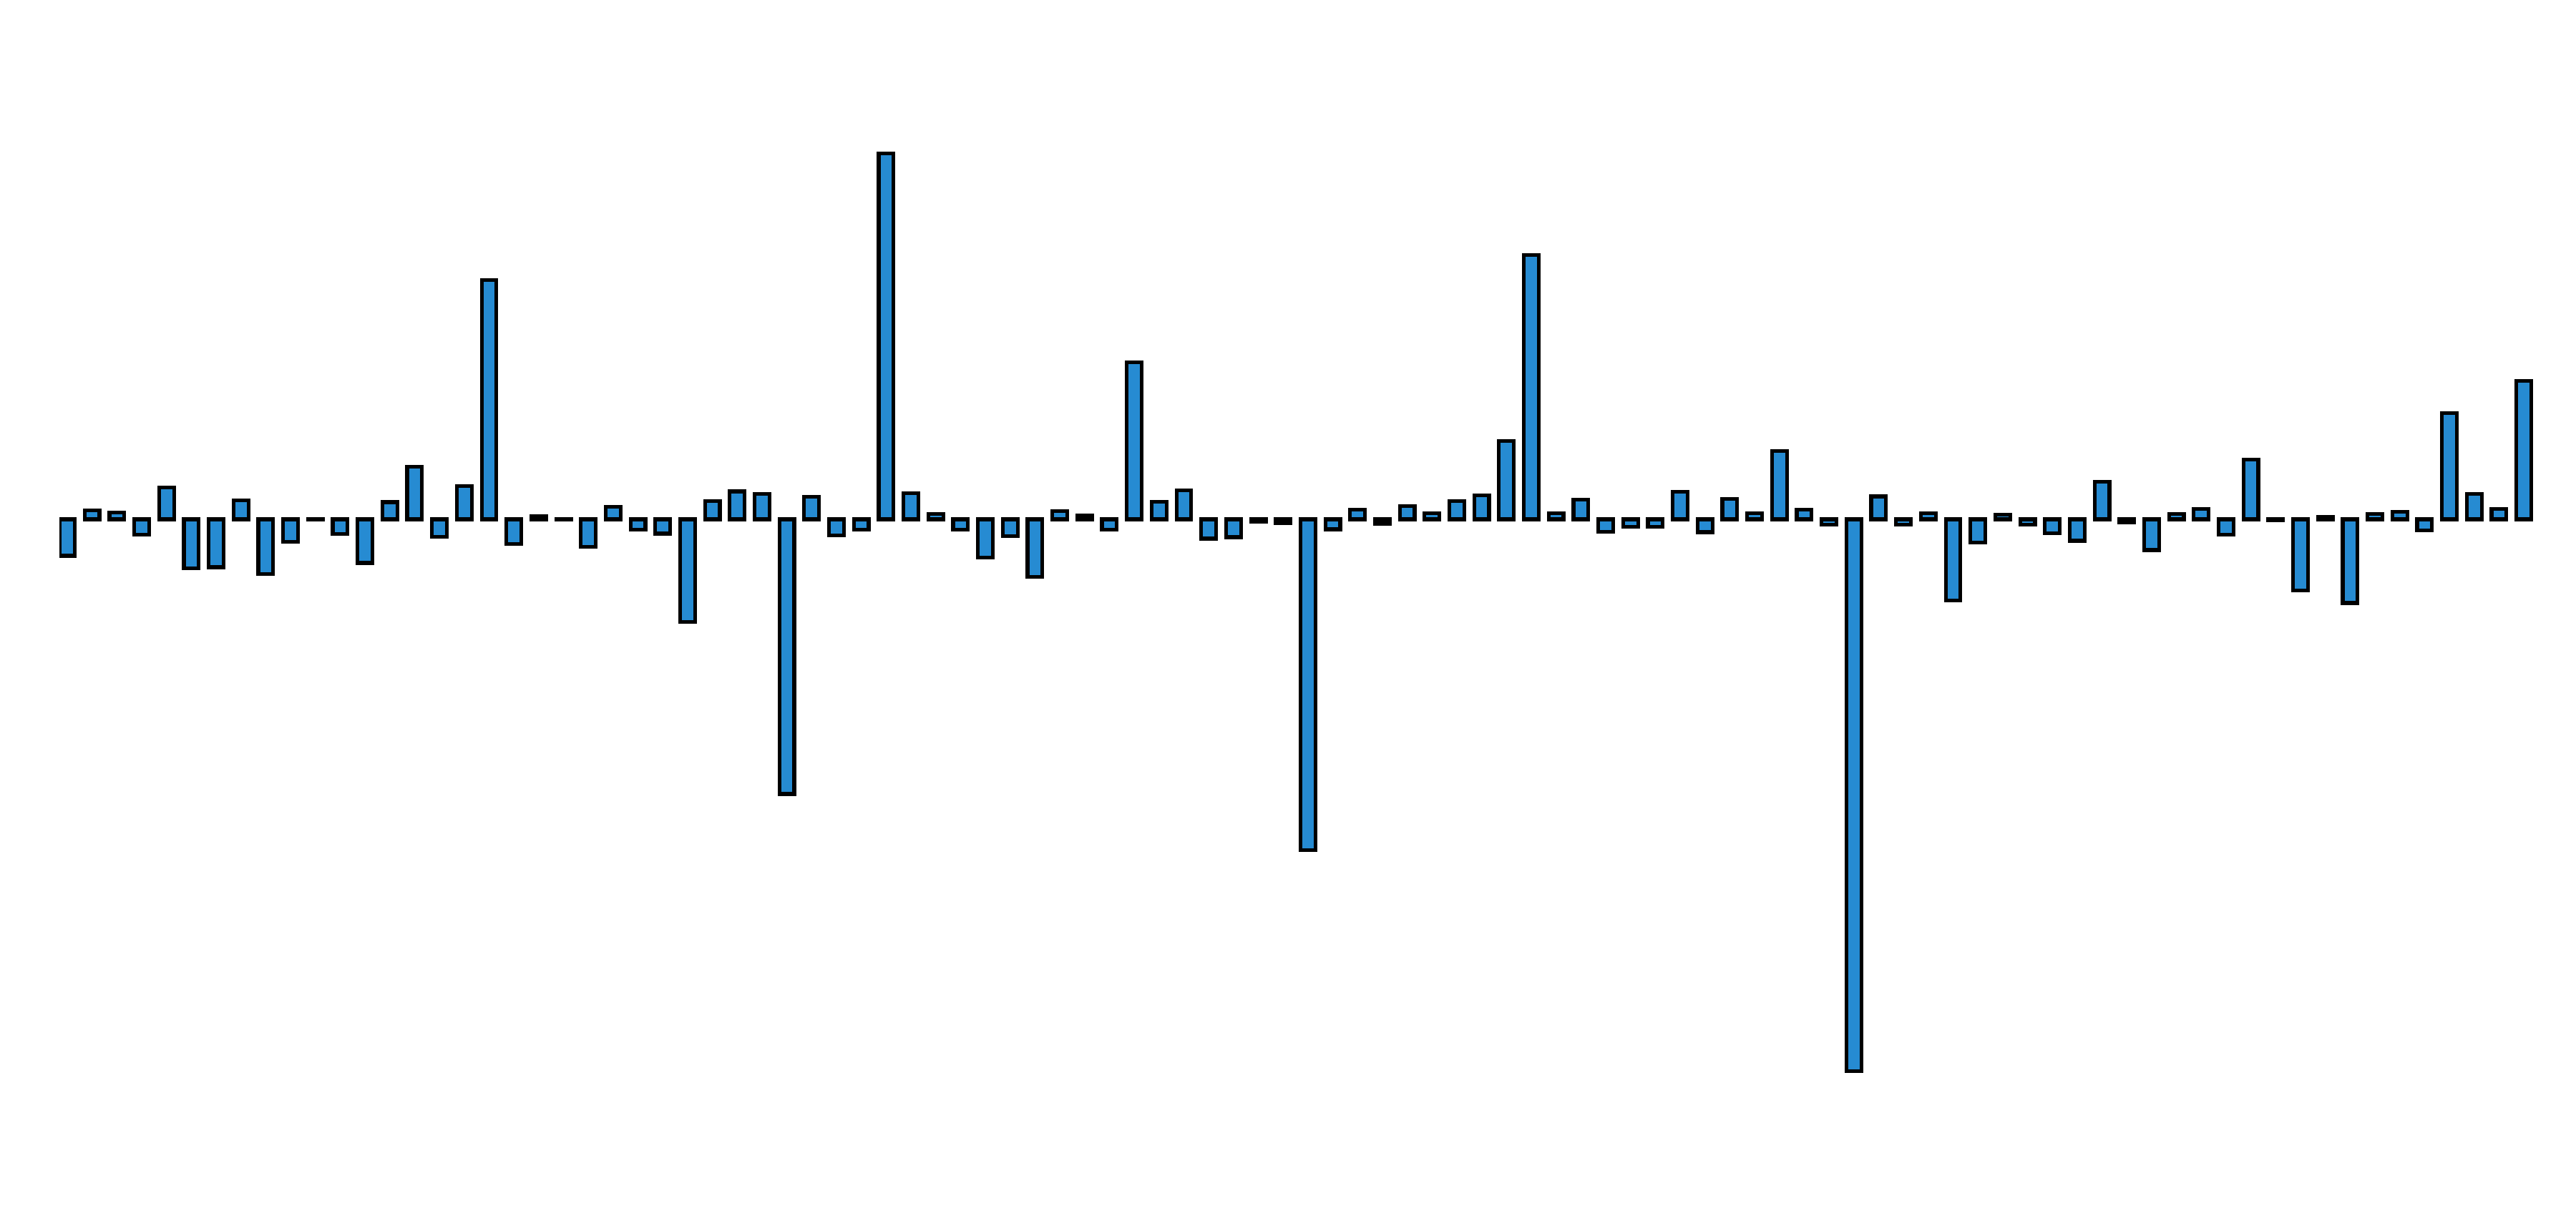
\includegraphics{LevyFlight/levy_length.pdf}
    \end{center}
    \caption{Distribution de 100 tirages aléatoire obéissant à une distribution de Lévy.
             \label{fig:levy_length}}
\end{figure}

\begin{figure}
    \begin{center}
        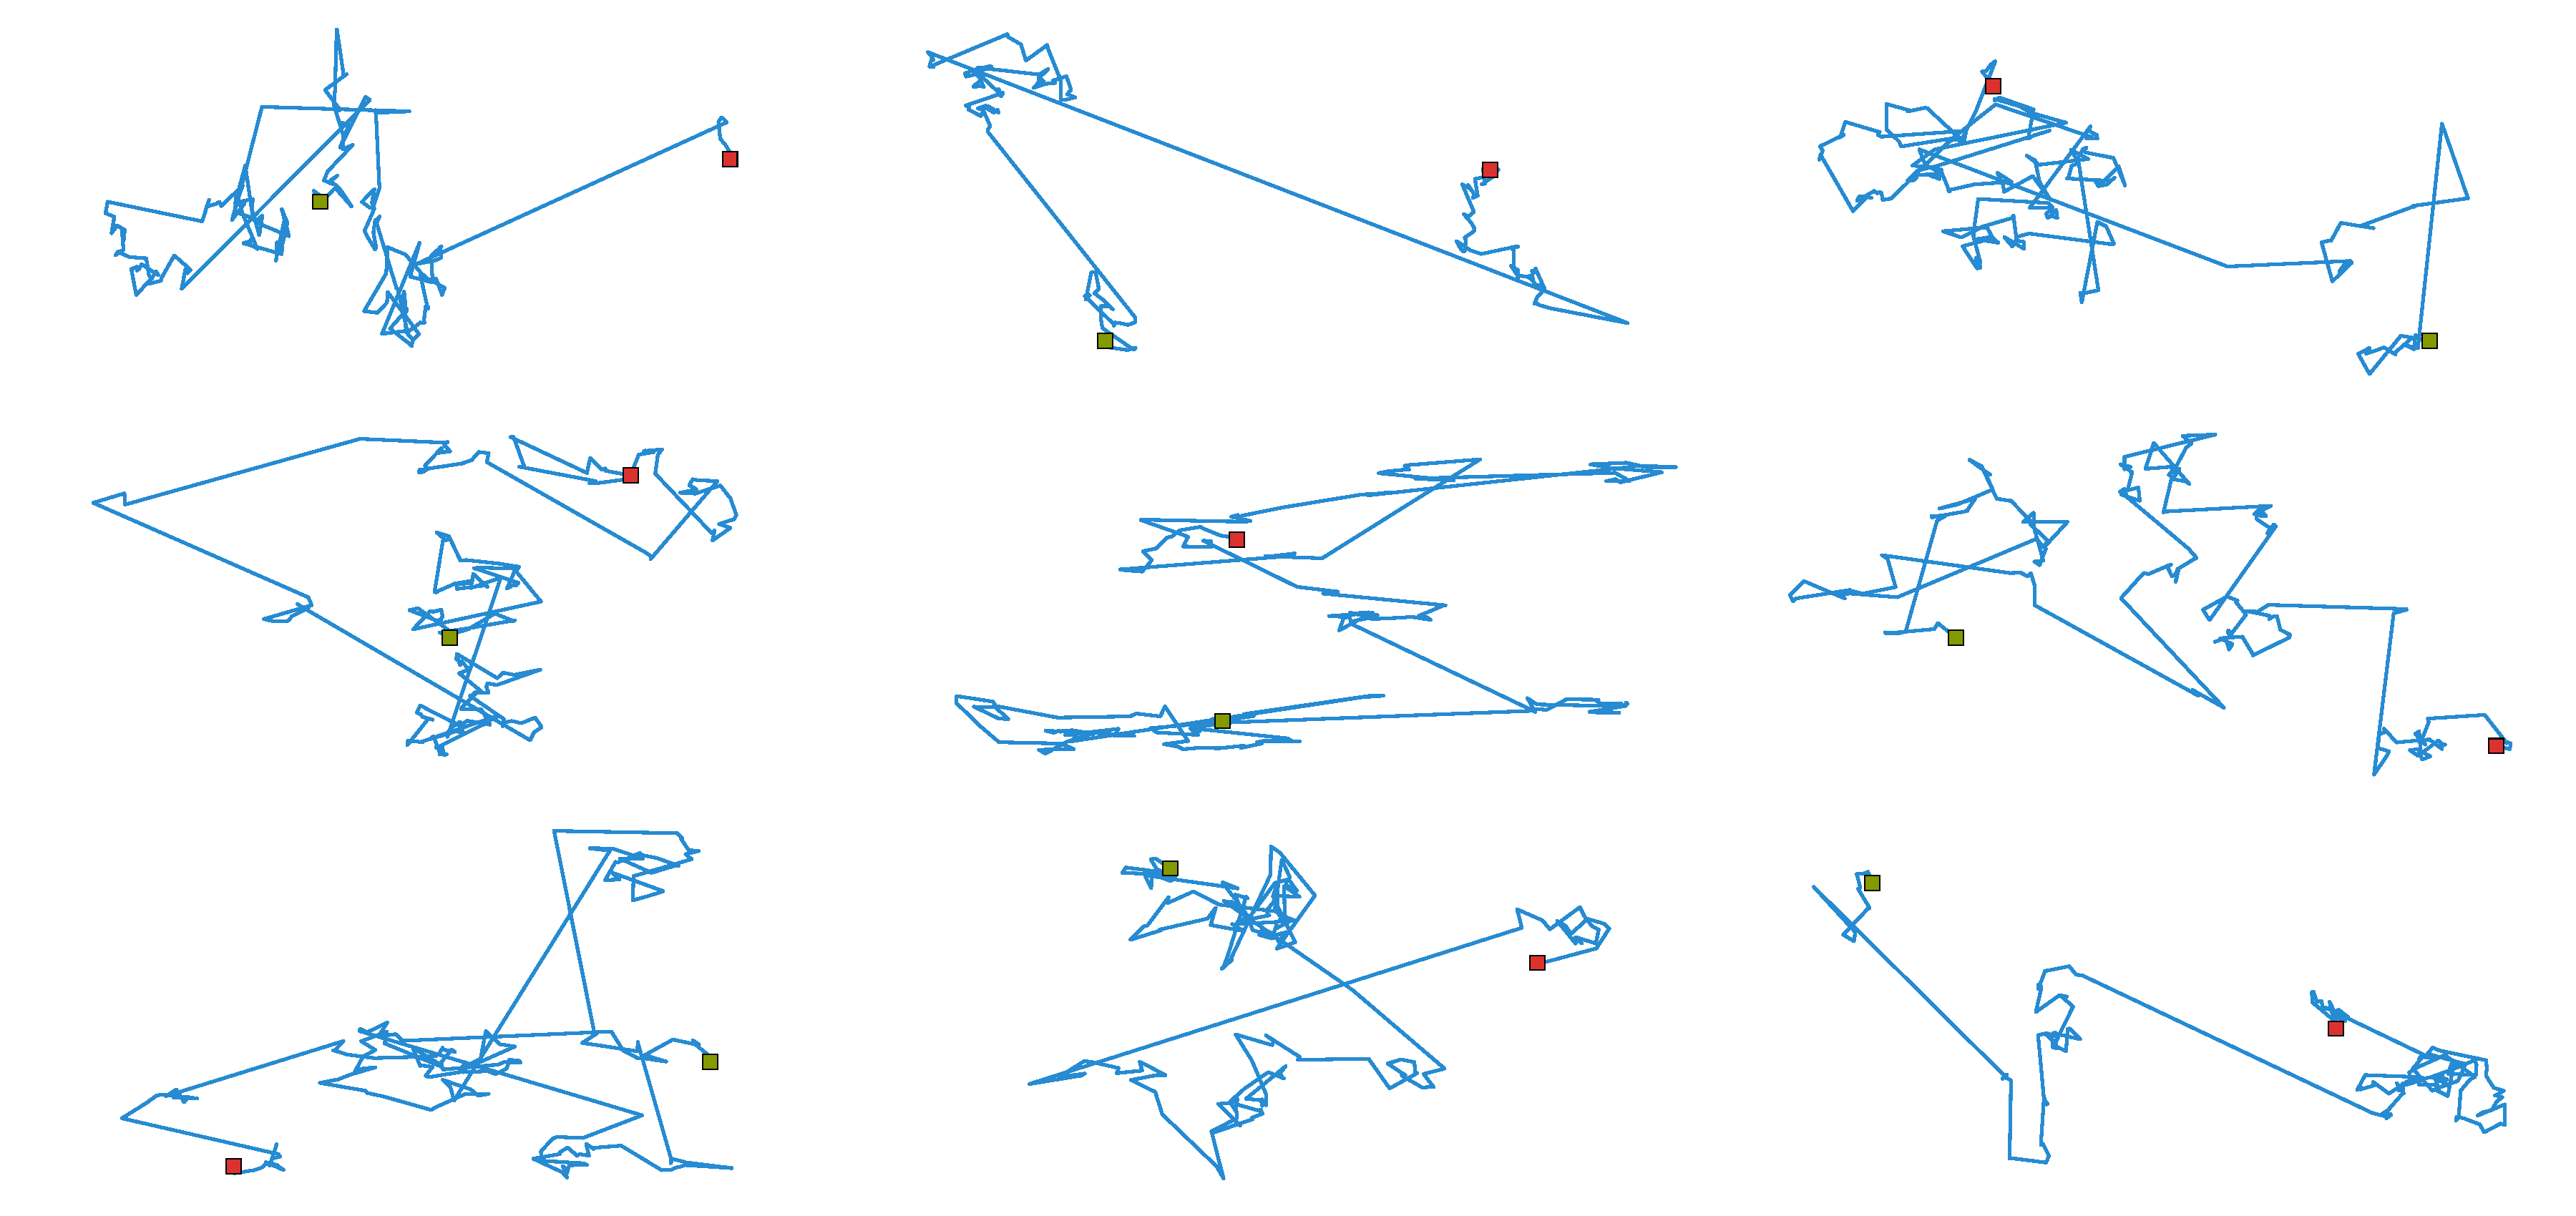
\includegraphics{LevyFlight/levy_flight.pdf}
    \end{center}
    \caption{Multiples vols de Lévy de 200 pas.
             \label{fig:levy_flight}}
\end{figure}

\begin{figure}
    \begin{center}
        \includegraphics{LevyFlight/levy_vs_gaussian.pdf}
    \end{center}
    \caption{Mouvement browien (en vert) et vol de Lévy (en bleu) pour 200 pas aléatoires.
             \label{fig:levy_vs_gaussian}}
\end{figure}

\itodo{Ajouter des applications aux problèmes multi-critères}
Dans \cite{Sharma2012213}, vol de Lévy est employé pour améliorer l’algorithme ABC
pour faire une recherche locale autour de la meilleure solution actuelle. L’auteur
utilise un multiplicateur pour réduire la longueur des pas généré d’après \eqref{eq:step_len}.
De plus la meilleure solution actuelle est utilisée pour guider la recherche aléatoire et
peu être assimilé à un apprentissage. Le vol de Lévy a aussi été utilisé dans un algorithme
d’optimisation approchée, le Cuckko search. Cet algorithme est inspiré du comportement
parasitaire de la reproduction des cuculidés et a était adapté aux problèmes
multi-critères (\cite{Yang20131616}).
% subsubsection vol_de_lévy (end)


% ------------------------------------------------------------------------------
\subsubsection{Apprentissage par opposition} % (fold)
\label{ssub:apprentissage_par_opposition}

La recherche par vecteur opposé (opposition-based learning) a été implémenté pour la première fois
en optimisation par \cite{Tizhoosh2005695,Rahnamayan2008155}. Il propose une méthode permettant de diversifier la
population sans connaissances à-priori.
% Opposite based learning method
\begin{Def}[OBLM~:~Opposition-Based Learning Method]\label{def:oblm}
La recherche par vecteur opposé (Opposition-Based Learning) permet de diversifier la
population sans connaissances à-priori.
Admettons un point de dimension $D$, $P(x_{1}, x_{2}, ..., x_{D})$ avec
$x_{1}, x_{2}, ..., x_{D}$ des valeurs bornées. Si $x_{i} \in [a_{i}, b_{i}]$ pour
$i = 1, 2, ..., D$ alors le point opposée est $\check{P}(\check{x_{1}}, \check{x_{2}}, ..., \check{x_{D}})$ suivant:
\[\check{x_{i}} = a_{i} + b_{i} - x_{i}\]
\end{Def}

Il est important de noter que les solutions sont comparées deux à deux par tournoi binaire, où
seule la meilleure solution entre l’initiale et son opposée est conservée. Admettons une solution
candidate $P(x_{1}, x_{2}, ..., x_{D})$ et son opposée $\check{P}(\check{x_{1}}, \check{x_{2}}, ..., \check{x_{D}})$,
alors si $f(\check{P}) \geq f(P)$ alors la solution $P$ est remplacé par $\check{P}$.
\ftodo{Illustration du tournoi binaire graphiquement}

Cette méthode a ensuite été améliorée (\cite{Rahnamayan2008155}) puis adaptée à
l’algorithme Differential evolution (DE). La méthode reprend la définition de base
mais définit plus clairement les limites et la portée de la méthode.
La méthode est utilisée durant la phase d’initialisation pour améliorer la diversité
en générant une population aléatoire de $n$ individus puis $n$ opposées.
Les solutions les plus performantes étant ensuite conservées pour obtenir une population
finale de $n$ individus.
Ensuite durant l’exécution de l’algorithme de nouvelles populations opposées sont générées.
Un coefficient $J_r$ est utilisé pour contrôler la probabilité de générer cette nouvelle
population opposée pour chaque itération.

La méthode a ensuite été testée sur un jeu de 15 fonctions de références (7 uni-modales
et 8 multi-modales). La nouvelle approche permet alors de trouver de meilleurs
résultats sur 14 des 15 fonctions. Il est aussi montré la supériorité de la
sélection par opposition par rapport au caractère aléatoire (\cite{Rahnamayan2008155,Rahnamayan2008906})
Il est aussi mis en avant que la probabilité de générer une population opposée
doit décroitre au fur et à mesure des itérations. En effet, la méthode permet de
réduire l’espace de recherche mais ralenti la convergence une fois cette intervalle
faible. Finalement il est proposé une intervalle de performance pour le coefficient si le problème
ne permet pas de déterminer un nombre fixe d’itération à-priori: $[0.1 < J_r < 0.4]$.

Cette approche a été appliquée avec succès dans le cas de l’algorithme ABC en couplage
avec un opérateur de mutation (\cite{Bi2011174}) ou encore en coopération avec une marche
aléatoire (\cite{Sharma2012213}).
Il a aussi été appliqué pour résoudre des problèmes plus complexe à objectifs multiples,
en combinaison avec un algorithme évolutionnaire (\cite{Ma201448}), ou encore avec le PSO (\cite{Gao2013114}).

Notre problème ne nous permettant pas d’avoir de connaissance à-priori, il nous est
impossible d’estimer le nombre d’itération nécessaires et l’utilisation d’un coefficient $J_r$
dynamique difficile.
% Au vu des recommandations et des applications déjà faites pour des problèmes mono-critères,
% ce coefficient sera fixé à 0.1 dans un premier temps.

\begin{figure}
    \begin{center}
        \includegraphics{abc/principe_obl.pdf}
    \end{center}
    \caption{Principe de fonctionnement de la recherche par vecteur opposée.
             \label{fig:OBL_method}}
\end{figure}

% subsubsection apprentissage_par_opposition (end)


\itodo{Décrire certaines approches parallèles (elle ne sont pas parallèle dans le sens que je veux faire)}
% subsection optimisation_par_essaim_d_abeilles_un_meta_heuristique_a_population (end)





\subsection{Mise à jour du front de Pareto} % (fold)
\label{sub:mise_a_jour_du_front_de_pareto}
L’une des principales difficultés lors d’une optimisation multi-objectif est de
déterminer quelles solutions conservées sachant que autant objectif n’est prioritaire.
Si tel était le cas, le problème pourrait être formuler sous la forme d’une optimisation
à objectif unique en ajoutant des poids aux divers objectifs par exemple.
La conservation de l’ensemble des solutions n’est pas une solution convenable. Des
solutions trop similaires vont parasiter l’efficacité de la recherche et ralentir la
convergence à cause d’un nombre conséquent de solution "clone".
Ainsi de nombreuses solution on cherché à définir des solution permettant de trier
le front de Pareto à chaque itérations pour converger efficacement vers le vrai front
de Pareto tout en assurant une bonne répartition sur celui-ci (\cite{Laumanns2002263}).
La mise à jour du front de Pareto doit ainsi
\\

Couramment utilisé, le \emph{Elitist Non-Dominated
Sorting Genetic Algorithm} (NSGA-II, \cite{Deb2002182}) s’articule en 3 étapes:
(i) classement des solutions du front précédent plus les nouvelles solutions
en niveau en fonction de leur dominance (Fast Nondominated Sorting Approach),
(ii) la mesure de la distance moyenne normalisée pour chaque
solution, tenant compte de tous les objectifs (crowing distance assignment), (iii)
la sélection de solution pour former le nouveau front (crowed-comparaison).
Dans cette approche les solutions de rang faible (non-dominées ou faiblement)
sont prioritaires. La taille de l’archive étant fixe, les solutions appartenant au
même rang sont triées selon le critère de distance. La compléxité de l’approche
étant alors de $\mathcal{O} \left (MN^{2} \right)$ avec $M$ le nombre d’objectifs.
\ftodo{Ajout de l’image descriptive du trie de cette approche (voir Deb2002182)
       avec des modifications pour la rendre plus compréhensive}
La méthode utilisée dans \emph{Strength Pareto Evolutionary Algorithm} (SPEA, \cite{Zitzler1999257})
est elle plus complexe, la distance euclidienne est utilisée pour former $N$ cluster
avec $N$ le taille de l’archive. Elle permet
d’obtenir une meilleure diversité que l’approche par NSGA-II mais est d’ordre plus
important ($\mathcal{O} \left (N^{3} \right)$) et demande donc plus de temps de calcul.

\cite{Laumanns2002263} propose de séparer l’espace des solutions en une grille en ajoutant la notion
de $\epsilon$-dominance. Dans cette approche l’espace des objectifs est divisé en hypercubes,
et chaque hypercube est comparé selon l’$\epsilon$-dominance. D’autres approches
utilisent une grille pour la mise à jour du front de Pareto (PAES, \cite{Knowles2000149}) mais
sans limiter le nombre de solutions par hypercubes limitant l’espace des objectifs. Ici,
chaque hypercube accepte une unique solution; la taille de l’archive est alors dépendante de la valeur
$\epsilon$ choisie pour chaque objectif.

\begin{figure}
    \begin{center}
        \includegraphics{abc/selection_boxes.png}
    \end{center}
    \caption{Principe de la mise à jour de l’archive par epsilon-dominance (maximisation assumée).
             \label{fig:epsilon_dominance}}
\end{figure}
L’archive (Fig.~\ref{fig:epsilon_dominance}) accepte une unique solution par hypercube dont la taille est définie par le
choix des epsilon (la tolérance de chaque objectif).
Lors de l’ajout d’une solution à l’archive on va ainsi en premier lieu vérifier que
l’hypercube à laquelle elle appartient n’est pas dominé. Si il est non-dominé la
nouvelle solution est ajoutée. Cependant si la solution est dans un hypercube contenant
déjà une solution, alors il est nécessaire de choisir entre les deux.
Ce choix peut être fait de deux manières: (i) On calcule la dominance stricte entre les
deux solutions, (ii) On calcule la distance euclidienne entre le coin supérieur droit
(dans le cas d’une maximisation) et les deux solutions, et on conserve celle ayant
la distance la plus faible.
Cette approche permet de garantir une diversité sur l’ensemble de l’espace de
décision pour un temps de calcul très faible.

\cite{Deb2005501} implémente la méthode et la compare à 4 autres approches dont SPEA2 et NSGA-II.
La comparaison prend en compte la convergence, la diversité des solutions, et le temps
de calcul nécessaire. Nommé $\epsilon$-MOEA, l’algorithme se révèle performant sur les
trois aspects évalués. Il peut être considéré comme un bon compromis entre la qualité
de la diversité apportée par les approches par clustering (SPEA2, C-NSGA-II), et la
vitesse de convergence des approches très élitistes (PESA, NSGA-II) pour un temps de
calcul bien inférieur. L’approche $\epsilon$-MOEA a cependant du mal à trouver des
solutions sur les extrêmes du front de Pareto à cause de la limitation du nombre de
solution par hypercube.
% subsection mise_a_jour_du_front_de_pareto (end)




\subsection{Réduction de la cardinalité par screening} % (fold)
\label{sub:reduction_de_la_cardinalite_par_screening}
% Analyse de sensibilité retenue:
%  - Formulation théorique
%  - Graphiquement
\itodo{Présenter l’analyse de sensibilité choisie ...}
% subsection reduction_de_la_cardinalite_par_screening (end)




\subsection{Processus d’optimisation complet} % (fold)
\label{sub:processus_d_optimisation_complet}
\itodo{Ajouter une vision globale du processus d’optimisation sous forme de graphique
      servant de résumé du chapitre.}


L’algorithme ABC modifié (Fig.~\ref{fig:abc_modifie}) comprend les même phases que l’original. La différence réside
dans le déroulement de ces phases. En effet plusieures technique présentées ci-avant
ont été implémentées afin d’améliorer l’exploitation et l’exploration de l’algorithme.
Enfin une archive par $\epsilon$-dominance est utilisé pour maintenir les solutions
non-dominées formant le front de Pareto. Cette archive est mise à jour après chaque
évaluation contrairement aux sources qui ne sont mis à jour que après chaque phase.

\begin{figure}
    \begin{center}
        \includegraphics[width=10cm, height=15cm]{abc/algorithme_complet.png}
    \end{center}
    \caption{Description globale de l’algorithme ABC modifié. Chaque phase renvois à un algorithme.
             \label{fig:abc_modifie}}
\end{figure}

Dans un premier temps l’algorithme initialise l’archive grâce aux objectifs et aux valeurs
d’epsilons. Ensuite la population est initialisé aléatoirement et une approche par OBL est
utilisée pour obtenir une meilleure diversité (Algorithm~\ref{alg:init_phase}). Ensuite on rentre dans la boucle principale
tant que la ou les conditions d’arrêts ne sont pas atteintes. Les différentes phases
sont les suivantes: (i) Phase des butineuses (Algorithm~\ref{alg:employed_phase}) qui explore l’espace de décision avec des vols de
Lévy, (ii) Phase des ouvrières (Algorithm~\ref{alg:onlooker_phase}) qui utilisent les informations acquises par les butineuses
et améliorent les sources choisies \eqref{eq:attribution_prob_to_source}, (iii) Phase des éclaireuses
(Algorithm~\ref{alg:scout_phase}) qui réinitialisent une source si elle est non fructueuse.
La longueur du vol de Lévy est définie par:
\begin{equation}\label{eq:levy_flight}
  LevyFlight = scaleFactor \times stepLength \times RandUniform(0, 1)
\end{equation}
avec $stepLength$ définie par \eqref{eq:step_len} et $scaleFactor$ fixé à 0.01.\\


% Attribution des probabilités
La probabilité de choisir une source $k$ par une ouvrière est elle définie comme:
\begin{subequations}\label{eq:attribution_prob_to_source}
  \begin{align}
    prob_{k} = &\frac{Qualite(\vec{x}_{k})}{\sum_{i=1}^{NbrSources} Qualite(\vec{x}_{i})} \\[1em]
    Qualite(\vec{x}_{k}) = &\frac{Dominance(k)}{NbrSources}
  \end{align}
  avec \emph{Dominance(k)} le nombre de source que la source $k$ domine, et \emph{Fitness}
  la qualité de la source en tenant comptes des contraintes comme définies en.
\end{subequations}

% Phase d’initialisation
\begin{algorithm}\label{alg:init_phase}
  \SetAlgoVlined
  \emph{Initialisation des sources sur l’ensemble de l’espace de décision}\;
  \For{$i \leftarrow 0$ \KwTo \ANbrSources}
  {
    \emph{Initialisation des critères pour chaque source}\;
    \For{$j \leftarrow 0$ \KwTo \ANbrCriteria}
    {
      \AComment{Génération aléatoire de la position initiale}
      $x_{ij} = x_{j}^{min} + RandUniform(0, 1) \times (x_{j}^{max} - x_{j}^{min})$\;
      avec $RandUniform$ un tirage aléatoire suivant une loi uniforme, et $x_{j}^{min}$, $x_{j}^{max}$
      respectivement le minimum et le maximum du critère $j$\;
      \vspace{1em}  % Add some space between two blocs
      \AComment{Génération de la position opposée suivant Definition~\ref{def:oblm}}
      $ \check{x_{ij}} = a_{j} + b_{j} - x_{ij}$\;
      avec $a_{j}$, $b_{j}$ respectivement les bornes inférieures et supérieurs du critère
    }
    \If{$\ASource_{i}$ respecte toutes les contraintes}
    {
      \AComment{On ajoute la source initial à l’archive}
      $\AArchive \pluseq \ASource_{i}$\;
    }
    \If{$\check{\ASource_{i}}$ respecte toutes les contraintes}
    {
      \AComment{On ajoute la source opposée à l’archive}
      $\AArchive \pluseq \check{\ASource_{i}}$\;
    }
  }
  \AComment{On ne conserve que une seule position par source}
  Mise à jour de la position des \ASources d’après Algorithm~\ref{alg:maj_phase}\;
  \caption{Initialisation des sources par OBLM (Opposite-Based Learning Method).}
\end{algorithm}

% Maj des sources
\begin{algorithm}\label{alg:maj_phase}
  \SetAlgoVlined
  Récupérer le maximum et minimum pour chaque objectif\;
  Récupérer le maximum pour chaque contrainte\;
  \For{$i \leftarrow 0$ \KwTo \ANbrSources}
  {
    Normaliser les objectifs et les contraintes avec ()\;
    Calculer la valeur de distance $\vec{d_{i}}$ en utilisant \eqref{eq:distance_measure}\;
    Calculer la pénalité $\vec{p_{i}}$ d’après ()\;
    \AComment{Attribuer les nouvelles valeurs d’objectifs aux sources}
    $\vec{F_{i}} = \vec{d_{i}} + \vec{p_{i}}$\;
    \If{$\check{\vec{F_{i}}} \succ \vec{F_{i}}$}
    {
      \AComment{On remplace la position de la source par la nouvelle}
      $\vec{x_{i}} \leftarrow \check{\vec{x_{i}}}$\;
      \AComment{On réinitialise le nombre d’échec pour la source $i$}
      $\ATrial_{i} \leftarrow 0$\;
    }
    \Else
    {
      \AComment{On incrémente le nombre d’échec pour la source $i$}
      $\ATrial_{i} \pluseq 1$\;
    }
    avec $\vec{F_{i}}$, $\check{\vec{F_{i}}}$ respectivement les vecteurs objectifs
    normalisés pour l’ancienne et la nouvelle position.\;
  }
  \caption{Mise à jour des sources}
\end{algorithm}

% Phase des butineuses
\begin{algorithm}\label{alg:employed_phase}
  \SetAlgoVlined
  \AComment{Exploration des sources par les \AEmployed}
  \For{$i \leftarrow 0$ \KwTo \ANbrSources}
  {
    Sélection aléatoire d’une source $k$ dans l’\AArchive\;
    \AComment{Génération d’une nouvelle position pour la \ASource $i$}
    \For{$j \leftarrow 0$ \KwTo \ANbrCriteria}
    {
      \begin{algomathdisplay}
        \check{x_{ij}} =%
          \begin{cases}
            x_{ij} + \ALevyFlight_{ij} \times (x_{ij} - x_{kj}) &\ \ATirage < \AMR \\
            x_{ij}                                      &\ sinon
          \end{cases}
      \end{algomathdisplay}
      avec \ATirage un nombre aléatoire uniforme (entre 0 et 1),
      \AMR un paramètre contrôlant le nombre de modifications
      et \ALevyFlight définie par \eqref{eq:levy_flight}\;
    }
    \If{aucun critère n’a été modifié}
      {
        \AComment{Sélection aléatoire d’un critère $j$ à mettre à jour}
        $\check{x_{ij}} = x_{ij} + \ALevyFlight_{ij} \times (x_{ij} - x_{kj})$\;
      }
    \If{$\ASource_{i}$ respecte toutes les contraintes}
    {
      \AComment{On ajoute la source initial à l’archive}
      $\AArchive \pluseq \ASource_{i}$\;
    }
    \If{$\check{\ASource_{i}}$ respecte toutes les contraintes}
    {
      \AComment{On ajoute la source opposée à l’archive}
      $\AArchive \pluseq \check{\ASource_{i}}$\;
    }
  }
  \AComment{On ne conserve que une seule position par source}
  Mise à jour de la position des \ASources d’après Algorithm~\ref{alg:maj_phase}\;
  \caption{Phase des butineuses.}
\end{algorithm}

% Phase des ouvrières
\begin{algorithm}\label{alg:onlooker_phase}
  \SetAlgoVlined
  \AComment{Exploitation des sources par les \AOnlookers}
  \For{$\ABee \in \AOnlookers$}
    {
      Sélection aléatoire d’une \ASource $i$ selon la probabilité
      définie par l’équation \eqref{eq:attribution_prob_to_source} (Sélection par roulette)\;
      Génération d’une nouvelle position pour la \ASource $i$ selon Algorithm~\ref{alg:employed_phase}
      (lignes 3 à 16)\;
    }
  \AComment{On ne conserve que une seule position par source}
  \AComment{Plusieurs \AOnlookers peuvent modifier la même source}
  Mise à jour de la position des \ASources qui ont été modifiées d’après Algorithm~\ref{alg:maj_phase}\;
  \caption{Phase des ouvrières.}
\end{algorithm}

% Phase des éclaireuses
\begin{algorithm}\label{alg:scout_phase}
  \SetAlgoVlined
  \For{$i \leftarrow 0$ \KwTo \ANbrSources}
  {
    \If{$\ATrial_{i} > \AMaxTrial$ }
    {
      \AComment{Exploration par les \AScouts}
      Génération de deux nouvelles positions suivant Algorithm~\ref{alg:init_phase}
      (lignes 4 à 16)\;
    }
  }
  \AComment{On conserve la meilleure solution parmi les deux nouvelles}
  Mise à jour de la position des \ASources d’après Algorithm~\ref{alg:maj_phase}\;
  \caption{Phase des éclaireuses.}
\end{algorithm}


% subsection processus_d_optimisation_complet (end)



\chapter{Analyse des résultats}

\section{Étude de sensibilité} % (fold)
\label{sec:etude_de_sensibilite}
Bénéfice de la méthode:

 - Rappel des critères en amont de l’étude
 - Sélection des critères en aval de l’étude de sensibilité
% section etude_de_sensibilite (end)


\section{Optimisation} % (fold)
\label{sec:optimisation}
Discussion sur le front de Pareto obtenu:

 - Analyse de la répartition des solutions
 - Analyse de la convergence
 - Analyse des résultats
% section optimisation (end)


\chapter*{Conclusion}
%!TEX root = ../main.tex

Oui c’est la fin, le grand final !!

Ouverture:
Évaluer la pertinence des fichiers météos pour un dimensionnement solaire
Aide à la décision par des méthodes plus poussées
Méthode de **clustering** pour évaluer le comportement hivernal et estival sur une
longue période.



% Start importing appendix
\appendix
\chapter{Appendix Title}
\include{Annexes/TestAnnexe}


% Add bibliography
\printbibliography

\end{document}
% ------------------------------------------------------------------------------
% Document end here
% ------------------------------------------------------------------------------


% Le surlignage empêche le retour à la ligne
% Refaire l’organisation entre chapitre 2 et 4 sinon il y aura des doublons.
